\documentclass[twoside, 12pt]{iiser-thesis}
\usepackage{graphicx}
\usepackage{amsmath}
\usepackage{amssymb, amsthm, thmtools, amsfonts}
\usepackage[dvipsnames]{xcolor}
%Command for theorems and stuff
\theoremstyle{definition}
\newtheorem{theorem}{Theorem}[section]
\newtheorem{corollary}{Corollary}[theorem]
\newtheorem{lemma}[theorem]{Lemma}
\newtheorem{proposition}[theorem]{Proposition}
\newtheorem{remark}[theorem]{Remark}
\theoremstyle{plain}
\newtheorem{definition}[theorem]{Definition}
\declaretheorem[style = plain, qed = $\lozenge\blacklozenge\lozenge$, numberwithin = section]{example}

\usepackage{layout}

%tikzpicture
%text width is 433pt
\usepackage{tikz}
\usepackage{scalerel}
\usepackage{pict2e}
\usepackage{tkz-euclide}
\usetikzlibrary{calc}
\usetikzlibrary{patterns,arrows.meta}
\usetikzlibrary{shadows}
\usetikzlibrary{external}
\usepackage{tikz-cd}

%pgfplots
\usepackage{pgfplots}
\pgfplotsset{compat=newest}
\usepgfplotslibrary{statistics}
\usepgfplotslibrary{fillbetween}
\usepackage[framemethod=TikZ]{mdframed}
%references package
\usepackage{hyperref}
\hypersetup{
    colorlinks=true,
    allcolors=blue}

%Thesis Preamble

\title{Tropical and Algebraic Geometry}
\author{Aditya Marodia}
\coordinator{Coordinator} \supervisor{Dr. Vivek Mohan Mallick} \sdesignation{Associate Professor}
\department{Department of Mathematics} \reader{Dr. Amit Hogadi}
%\reader{Reader 2}
\dedication{This thesis is dedicated to my sister, Aanya}
\graduationyear{2025}
\academicyear{2024-2025}
\graduationmonth{May}

\thesisabstract{
    Over the past few deccades Tropical Geometry has emerged as an enticing subfield of Algebraic Geometry. 
    In Tropical Geometry one often deals with combinatorial objects which come from algebraic varieties - retaining a lot of their original structure.
    In this thesis we look at Tropical Geometry and see how one can use Tropical methods to solve problems in Algebraic Geometry.
    The primary problem we look at in this thesis is the curve counting problem: how many curves of degree $d$ pass through $3d-1$ points in the plane?
    We study the original proof of this problem, given by Maxim Kontsevich - using the moduli space of stable maps.
    Then we allude to Mikhailkin's correspondence result, which showed that these numbers are the same in the Tropical world.
    We then look at proof of this result in the Tropical world and compare the methods used in this proof to those of Kontsevich's.
}
\acknowledgments{I would firstly like to thank my family for supporting me throughout my life, this thesis would not come to fruition without their presence.
    \par I have been in contact with Dr. Vivek Mallick for almost two years now, and his guidance not only has shaped this thesis but also helped me find my place in math. 
    Dr. Chandranandan Gangopadhyay has essnetially acted as a co-supervisor during my thesis - consistently attending my meetings, clarifying my queries and helping me learn.
    I would also like to thank Dr. Nitin Nitsure and Dr. Amit Hogadi who helped me start learning scheme theory during thesis.
    \par And finally, I could not have written this up without my friends - who were there for me when I felt mentally exhausted, who provided me company while studying and much more. 
}


%Start of document
\begin{document}

\thesisfront

\chapter{Preliminaries on tropical geometry}
\label{chapTrop}
\section{Introduction and Examples}
\subsection{Tropical Arithmetic}
    \begin{definition} The tropical semiring $(\mathbb{R} \cup \{\infty\}, \oplus, \odot)$, is defined as the semiring whose underlying set is $\mathbb{R}$ with the binary operations: 
        \begin{align*}
            x \oplus y &= \text{min}(x,y)\\
            x \odot y  &= x + y
        \end{align*}
    We refer to $\oplus$ as the \textit{tropical sum}, and $\odot$ as the \textit{tropical product}. This can be a little confusing since the tropical product is defined as out usual notion of sum.
    \end{definition}

\subsection{Tropical plane curves}
Just like in algebraic geometry, our source of geometric objects in the tropical world comes from polynomials.
We will look at how polynomials behave on the tropical semiring to get an idea of the geometric objects we will soon be dealing with.
For any polynomial $f  = \sum_{i}c_{i}x^{i}\in \mathbb{R}[x]$, the standard polynomial ring, the tropical analougue, $\text{trop}(f)$ is:
\begin{align*}
    \text{trop}(f) &= \bigoplus_{i}c_{i}\odot x^{\odot i}\\
                   &= \text{min}_{i}(c_{i} + i \cdot x),
\end{align*}
a piecewise linear function from $\mathbb{R}$ to $\mathbb{R}$.
\par \textcolor{red}{Insert Image of piecewise linear function}
\par Just like how we study the roots of polynomials in algrbaic geometry, in tropical geometry we care about the points in the domain where the tropical polynomial is \textit{not linear}.
This will be justified in remark \ref{rootValRmk} and the fundamental theorem in later sections.
\par The tropical polynomial in $2$ variables serve as a more instructive example to understand what the set of non-differentiable points look like. 
\textcolor{red}{[Add diagram and stuff for two variable polynomials]}

\begin{remark}
    \label{rmkOnTropPol}
    Note that the tropicalisation of polynomials in the rest of the thesis will be slightly different from the tropicalisations considered in this section.
    From now on we will be dealing with valuations and when we move the tropical world we will consider the valuations of the coeffiecients instead. 
    This will be elaborated upon in the next section.
\end{remark}

\subsection{Valuations and Varieties}
    \begin{definition}
        For a field $K$ we define the valuation $\emph{val}$ as a function $\emph{val}: K \to \mathbb{R}\cup \{\infty\}$ such that:
        \begin{enumerate}
            \item $\emph{val}(a) = \infty \Leftrightarrow a = 0$
            \item $\emph{val}(ab) = \emph{val}(a)+ \emph{val}(b)$
            \item $\emph{val(a+b)} \geq \emph{min}(\emph{val}(a),\emph{val}(b))$
        \end{enumerate}
        The image of $\emph{val}$ is an additive subgroup, $\Gamma_{\emph{val}} \subset \mathbb{R}$, called the value group.
        \par An important assumption we make is that $1 \in \Gamma_{\text{val}}$. 
    Further, we define $K^{\circ} := \{a \in K: \emph{val}(a)\geq 0\}$, and $K^{\circ \circ} := \{a \in K: \emph{val}(a)> 0\}$. 
    And the residue field $\tilde{K} := K^{\circ}/K^{\circ \circ}$.
    \end{definition}

    \begin{lemma}
        \label{vallemma}
        When $\text{val}(a) \neq \text{val}(b)$ for $a,b \in K$, then $\text{val}(a+b)= \text{min}(\text{val}(a),\text{val}(b))$.
    \end{lemma}
    It's not hard to see that the algebraic structure induced on the image of the valuation map is almost same as the algrbaic structure on the tropical semiring. 
    This observation motivates us to define tropicalisation of a polynomial with respect to a given valuation (as hinted in \ref{rmkOnTropPol}).
    For $f = \sum_{i}c_{i}x^{i} \in K[x]$ a polynomial in a valued field $(K, \text{val})$, the valued tropicalisation is defined as
    \begin{equation*}
        \text{trop}_{\text{val}}(f) = \text{min}_{i}(\text{val}(c_{i}) + i \cdot x).
    \end{equation*}
    \begin{remark}
        \label{rootValRmk}
    We now make a key observation. For any tropical polynomial (tropicalisation of a standard polynomial) in one variable, we refer to the points where it's not differentiable as its \textbf{roots}. 
    Suppose $f(x) = \prod_{i=1}^{n}(x-\lambda_i) \in K[x]$, where $K$ is some valued field, then $\text{trop}(f) = \sum_{i=1}^{n}\text{min}(\text{val}(x),\text{val}(\lambda_i))$. 
    It's clear that the \textbf{``roots"} of $\text{trop}(f)$ are $\text{val}(\lambda_i)$.
    This relation between the two types of \textit{roots} will be further generalised, and will lead to the \textit{fundamental theorem of tropical geometry}.
    \end{remark}

    \begin{lemma}
        Suppose $K$ is an algebraically closed valued field, then the value group $\Gamma_{\emph{val}}$ is divisible and dense in $\mathbb{R}$.
    \end{lemma}

    \begin{lemma}
        When $K$ is an algebraically closed valued field, the surjection $K^{*} \twoheadrightarrow \Gamma_{\emph{val}}$ splits.
    \end{lemma}

    The splitting is a map $\phi: \Gamma_{\text{val}} \to K^{*}$, but we always denote $\phi(w)$ with $t^w$. This notation is inspired from the splitting in the case where $K$ is the field of Puiseux series.
    \par Other than the standard affine and projective spaces, in tropical geometry we often deal with \textit{n-dimensional algebraic tori}: $T^{n}_{K} := T^n = (K^{*})^n$. 
    The coordinate ring of $T^{n}$ is $K[x_{1}^{\pm 1},\dots,x_{n}^{\pm 1}]$, the ring of laurent polynomials. 
    Zero set of ideals in the laurent polynomial ring define varieties in $T^n$, these varieties are called \textbf{very affine varieties}.
    Just like for affine spaces we can define a Zariski topology on $T^{n}$.
    \par We now have the inclusions $i: T^{n} \hookrightarrow \mathbb{A}^n$ and $j: \mathbb{A}^{n} \hookrightarrow \mathbb{P}^{n}$. 
    The affine closure of a very affine variety $X$ is $\overline{i(X)}$, and the projective closure of a affine variety $X$ is $\overline{j(X)}$. 
    For an ideal $I \subset K[x_{1}^{\pm 1},\dots,x_{n}^{\pm 1}]$, define $I_{\text{aff}}:= I \cap K[x_{1},\dots,x_{n}]$.

    \begin{proposition}
        For $I \subset K[x_{1}^{\pm 1},\dots,x_{n}^{\pm 1}]$ let $X = V(I) \subset T^n$, then $V(I_{\text{aff}}) = \overline{i(X)}$.
    \end{proposition}

    \begin{proposition}
        \label{densenessprop}
        $(K,v)$ be a valued field with splitting $\Gamma_{\emph{val}} \twoheadrightarrow \mathbb{R},~w \to t^{w}$.
        Let $\alpha_{1}, \dots,\alpha_{n} \in \tilde{K}^{*}$ and $w_1, \dots, w_n \in \Gamma_{\emph{val}}$. 
        Conisder the set of $\textbf{y} = (y_1, \dots, y_n) \in T^{n}$ such that $\emph{val}(y_{i}) = w_{i}$ and $\overline{t^{-w_i}y_i} = \alpha_{i}$ for all $1\leq i \leq n$.
        This set is dense in $T^n$ with respect to the Zariski topology.
    \end{proposition}

    \subsection{Polyhedral Geometry}
We now very quickly go through some elementray definitions and constructions in Polyhedral Geometry. 
This section very closely follows the exposition in section 2.3 of \cite{maclagan2015introduction}.
   \par A set $X\subset \mathbb{R}^{n}$ is said to be \textbf{convex} if for any two points in $X$ the line connecting those two points also lies in $X$. 
   The \textbf{convex hull}, conv$(U)$, of a set $U\subset \mathbb{R}^{n}$ is the smallest convex set containg $U$.
   When $U$ is a finite set $\text{conv}(U)$ is a \textbf{polytope}. 
   A \textbf{polyhedral cone} $C \subset \mathbb{R}^{n}$ is the \textit{positive hull} of a finite subset of $\mathbb{R}^{n}$. 
   For a set $U = \{u_1,\dots,u_n\}$:
   \begin{align*}
       C = \text{pos}(U) = \left\{\sum_{i=1}^{n}\lambda_i u_i~:~\lambda_i\geq 0\right\}
   \end{align*}
   When the $u_i$'s are linearly independent, the cone is said to be \textbf{simpilicial}. 
    It's easy to see that every polyhedral cone is a finite intersection of \textit{half n-spaces}, this perspective allows to define cones as the set $\{x \in \mathbb{R}^{n}: Ax\leq 0\}$, where $A$ is a $d \times n$ matrix. 
    For a dual vector $w \in (\mathbb{R}^{n})^{\vee}$ we define the associated face in the cone $C$ as:
    \begin{align*}
        \text{face}_{w}(C) = \left\{x \in C: w\cdot x \leq w\cdot y ~\text{for all}~y \in C\right\}
    \end{align*}
    For $d'$ the dimension of the face, there also exists a $d'\times n$ matrix $A'$ such that $\{x \in C: A'x\ =  0\}$. 
    A \textbf{polyhedral fan} is a collection of polyhedral cones such that every face of the cone is part of the collection, and the intersection of any two cones is a face of both the cones.
    A \textbf{polyhedron} $P \subset \mathbb{R}^{n}$ is the intersection of finitely many affine half spaces, allowing us to define it as the set $\{x \in \mathbb{R}^{n}: Ax\leq b\}$ where $b \in \mathbb{R}^{d}$ and $A$ is a $d \times n$ matrix. We can define faces of polyhedron's in the same manner as we defined faces of a cone.
    \par A \textbf{polyhedral complex}, $\Sigma$, is a collection of polyhedron such that: if $P \in \Sigma$ then all faces of $P$ also lie in $\Sigma$, and if $P,Q \in \Sigma$ then $P \cap Q = \emptyset$ or $P \cap Q$ is a face of both $P,Q$. The support of a polyhedral complex, $|\Sigma |$ is the underlying set of points in $\Sigma$. 
    The \textbf{lineality space} of a polyhedral complex, if it exists, is the largest linear subspace which lies in it.
    For any set of points in $\mathbb{R}^{n}$, their \textbf{affine span} is defined as the smallest affine subspace containing those points.

    The \textbf{regular subdivision} is an important construction since it helps us create a link between the newton polytope and tropical variety. 
    \begin{definition}
    For an ordered list of vectors $v_1,\dots, v_r \in \mathbb{R}^{n}$, fix a weight vector $w = (w_1,\dots,w_n) \in \mathbb{R}^{n}$. 
    The \textit{regular subdivision} is the polyhedral fan with support $\text{pos}(v_1,\dots,v_n)$ whose cones are $\text{pos}(\sigma)$ for all $\sigma \subset \{v_1,\dots,v_n\}$ such that there exists $c \in \mathbb{R}^{n+1}$ for which:
    \begin{itemize}
        \item $c \cdot v_i = w_i$ for all $v_{i}\in \sigma$ 
        \item $c \cdot v_i < w_i$ for all $v_i \not\in \sigma$
    \end{itemize}
    Although defined as a fan, regular subdivisions are usually defined for polyhedral complexes.
    \end{definition}
    Suppose you have a polyhedron $P$ given by $\text{conv}(u_i: 1\leq i\leq r)$, we look at the vectors $v_i = (u_i,1)$. 
    The regular subdivision of $v_1,\dots,v_r$ with respect to a weight vector $w = (w_1, \cdots, w_r)$ can be interpreted as projection of the bottom faces of the polytope $P_w = \text{conv}\{(u_i,w_i): 1\leq i\leq r\}$. 
    That is, in the polytope $P_w$ consider the faces $F$ whose normal vector has positive final coordinates and project them onto the first $r$ coordinates, this gives the regular subdivision of $P$ with respect to $w$.

\section{Tropical Hypersurfaces}

    \begin{definition}
        Consider polynomial $f = \sum c_u x^u \in K[x_0,\dots,x_n]$, and let
        \[
            W = \text{trop}(f)(w) = \text{min}_{u \in \mathbb{Z}^{n+1}}\{\text{val}(c_u) + u\cdot w\}.
        \]
        Then we define the initial form of $f$ with respect to $w$ as
        \begin{align*}
            \text{in}_{w}(f)(x) = \sum_{\text{val}(c_u) + u\cdot w = W} \overline{c_u t^{-\text{val}(c_u)}} x^u.
        \end{align*}
        We can also define the initial form for a laurent polynomial $f$ in the same way.
    \end{definition}

    It's easter to discuss properties of these initial forms once we understand their relation to tropical hypersurfaces.
    So before we further study these intial forms, we will first look at tropical hypersurfaces.
    \begin{definition}
        For a laurent polynomial $f \in  K[x_{1}^{\pm1}, \dots, x_{n}^{\pm1}] $, the tropical hypersurface $\emph{trop}(V(f))$ is the set:
        \begin{align*}
        \{w \in \mathbb{R}^{n}: \text{minimum in }\emph{trop}(f)(w)\text{ is acheived atleast twice}\}.
        \end{align*}
    \end{definition}
    Similarly, for a tropical polynomial $F$, $V(F)$ denotes the set:
    \begin{align*}
        \{w \in \mathbb{R}^{n}: \text{minimum in }F(w)\text{ is acheived atleast twice}\}.
    \end{align*}
    It's clear that for a laurent polynomial $f$: $V(\text{trop}(f)) = \text{trop}(V(f))$

    That next theorem gives various characterisations for a tropical hypersurface.
    The generalisation of this theorem to varieties of higher codimensions is called the \textit{fundamental theorem of Tropical Geometry}.
    \begin{theorem}[Kapranov's Theorem]
    Let $K$ be an algebraically closed field with a non-trivial valuation. Fix a laurent polynomial $f \in K[x_{1}^{\pm1}, \dots, x_{n}^{\pm1}]$. The following sets are the same:
    \begin{enumerate}
        \item $A$ = $V(\text{trop}(f))$.
        \item $B$ = $\{w \in \mathbb{R}^{n}: \text{in}_{w}(f)~ \text{is not a monomial}\}$.
        \item $C$ = closure of $\left\{(\text{val}(y_1), \dots, \text{val}(y_n)): (y_1,\dots, y_n) \in V(f)\right\}$ in $\mathbb{R}^{n}$.
    \end{enumerate}
    Further, if $f$ is irreducible and $w \in \Gamma_{\text{val}} \cap \text{trop}(V(f))$, then the set $\{y \in V(f): \text{val}(y) = w\}$ is Zariski dense in $V(f)$.
    \end{theorem}

    \begin{proof}[Sketch of proof]
        Showing $A$ = $B$ is straightforward. 
        If $x \in A$ then there exist atleast two $u_1,~u_2$ such that $\text{trop}(f)(x) = \text{val}(c_{u_{1}}) + u_{1}\cdot x = \text{val}(c_{u_{2}}) + u_{2}\cdot x$. 
        This implies $\text{in}_{x}(f)$ has atleast the terms corresponding to $u_1$ and $u_2$, implying it's not a monomial, and $A \subset B$.
        Now consider a $w \in B$, the initial form $\text{in}_{w}f = \sum_i \text{val}(c_{u_{i}}) + u_i \cdot w$ has atleast two terms, say for $i=1,2$. 
        Therefore $\text{trop}(f)(w) = \text{val}(c_{u_{1}}) + u_{1}\cdot w = \text{val}(c_{u_{2}}) + u_{2}\cdot w$, implying $w \in A$.
        Hence A = B.
        \par To show $C \subset A$, since $A$ is already closed, we just need to show that the set $\{(\text{val}(y_1), \dots, \text{val}(y_n)): (y_1,\dots, y_n) \in \mathbb{R}^{n}\}$ lies in $A$. Say $\textbf{y} = (y_1,\dots,y_n) \in V(f)$, this implies 
        \begin{align*}
            f(\textbf{y}) &= \sum_u c_u y^{u} = 0 \\
            \Rightarrow&\text{val}(\sum_u c_u y^{u}) = \infty \\
            \Rightarrow& \text{min}_u(\text{val}(c_u) + u \cdot \text{val(\textbf{y})}) = \infty
        \end{align*}
        For this equality to hold, for any pair $u_{1},~u_{2}$ with $c_{u_{i} \neq 0}$ we need to have $\text{val}(c_1) = \text{val}(c_2)$, else by [\ref{vallemma}] $\text{val}(f(\textbf{y})) < \infty$, which is a contradiction. 
        \par To finish of the proof, we show $B \subset C$ and the density statement in the next propostion.
    \end{proof}
    This proposition uses notation from the statement of Kapranov's Theorem.
    \begin{proposition}
        Fix a laurent polynomial $f \in  K[x_{1}^{\pm1}, \dots, x_{n}^{\pm1}]$, and let $w \in \Gamma_{\text{val}^{n}}$. 
        Suppose $w \in B$ and $\alpha \in (\tilde{K}^{*})^{n}$ satisfies $\text{in}_{w}(f)(\alpha) = 0$. 
        There exists $\textbf{y} \in (K^{*})^{n}$ such that $f(\textbf{y}) = 0$,  $\text{val}(\textbf{y}) = \textbf{w}$, and $t^{-1_{i}}y_{i}=\alpha_{i}$ for $1 \leq i \leq n$.
        Further, if $f$ is irreducible, then the set of such $\textbf{y}$ is Zariski dense in the hypersurface $V(f)$.
    \end{proposition}
    \begin{proof}
        We go about proving this proposition via induction on $n$.
        \par \textit{Base Case.} Consider $n = 1$.
        \par We can multiply by a unit and assume that $f = \sum_{i=0}^{s}c_{i}x^{i}$ such that $c_{0}, c_{s}\neq0$. 
        Since we are working in an algebraically closed field $K$, $f = \prod^{s}_{j=1} (a_{j}x-b_{j})$. 
        Then, $\text{in}_{w}(f) = \prod^{s}_{j=1} \text{in}_{w}(a_{j}x-b_{j})$. 
        Since $\alpha \in \tilde{K}$ and $\text{in}_{w}f(\alpha)=0$, there exists $j$ such that $\text{in}_{w}(a_{j}x-b_{j})(\alpha) = 0$.
        Futher, since $w \in B$, the initial form $\text{in}_{w}(f)$ is not a monomial.
        This implies that $\text{in}_{w}(a_{j}x-b_{j})$ is not a monomial, hence:
        \begin{align*}
            \text{val}(a_{j}) + w &= \text{val}(b_{j})\\
            \alpha &= \overline{t^{-w}b_{j}/a_{j}}.
        \end{align*}
        Setting $y = b_{j}/a_{j}$ we get $f(y) = 0$, and $\overline{t^{-\text{val}(y)}y} = \alpha$, proving the base case.
        \par \textit{Inducting on n}. Consider $n>1$.       
        We first show that there exists an automorphism on $\phi \in K[x_{1}^{\pm1}, \dots, x_{n}^{\pm1}]$ such that $\phi(f)$, when seen as a polynomial in $x_{n}$, has coefficients which are monomials in $ K[x_{1}^{\pm1}, \dots, x_{n-1}^{\pm1}]$. 
        It's easy to construct such a automorphism:
        \begin{itemize}
            \item Choose $l \in \mathbb{Z}_{>0}$.
            \item Define $\phi^{*}_{l}: K[x_{1}^{\pm1}, \dots, x_{n}^{\pm1}] \to  K[x_{1}^{\pm1}, \dots, x_{n}^{\pm1}]$ as:
                \begin{align*}
                    x_{i} &\mapsto x_{i}x_{n}^{l^{i}}~~\text{for }1\leq i\leq n-1\\
                    x_{n} &\mapsto x_{n}.
                \end{align*}
            \item Any monomial in the polynomial $f$ can be expressed as $x^{\textbf{u}}x_{n}^{r}$, where $\textbf{u} \in \mathbb{Z}^{n-1}$, and:
                \[
                    \phi^{*}_{l}(x^{\textbf{u}}x_{n}^{r}) = x^{\textbf{u}}x_{n}^{r+\sum_{i=1}^{n-1}l_{i}}.
                \]
            \item It's clear now that we can choose $l$ large enough such that each monomial of $f$ under $\phi^{*}_{l}$ has a unique exponent in $x_{n}$.
        \end{itemize}
        \par Hence, we have found an automorphism $\phi^{*}_{l}$ which satisfies the required propeties. If $\textbf{y}\in T^{n}$ satisfies:
        \begin{align*}
            \phi^{*}_{l}(f)(\textbf{y}) &= 0\\
            \text{val}({y}_{i}) &= w_{i} - l^{i}w_{n} \\
            \overline{t^{-w_{i}- l^{i}w_{n}}y_{i}} &= \alpha_{i}\alpha_{n}^{-l^{i}},
        \end{align*}
        then for  $\textbf{y}'\in T^{n}$, defined by $y'_{i}=y_{i}y_{n}^{l^{i}}$ for $1\leq i<n$, and $y'_{n}  = y_{n}$:
        \begin{align*}
            f(\textbf{y}') &= 0\\
            \text{val}({y'}_{i}) &= w_{i} \\
            \overline{t^{-w_{i}}y'_{i}} &= \alpha_{i}.
        \end{align*}
        Therefore we can replace $f$ with $\phi^{*}_{l}(f)$.
        By construction of $\phi^{*}_{l}$, we know that when $f$ is regarded as a polynomial in $x_{n}$, all coefficients are monomials in $ K[x_{1}^{\pm1}, \dots, x_{n-1}^{\pm1}]$.
        \par Consider the set $\mathcal{V} := \{(y_{1},\dots, y_{n-1})\in T^{n-1}: \text{val}(y_{i}) = w_{i},\,\overline{ t^{-w_{i}}y_{i}} = \alpha_{i} \}$.
        From proposition \ref{densenessprop}, we know that the set $\mathcal{V}$ is Zariski dense in $T^{n-1}$.
        Additionaly, for each such point $\textbf{y}\in \mathcal{Y}$ the polyomial defined by $g(x_{n}) = f(y_{1},\dots, y_{n-1}, x_{n})$ is non-zero.
        For $\textbf{u} \in \mathbb{Z}^{n}$ we denote with $\textbf{u}'\in \mathbb{Z}^{n-1}$ the projection of $\textbf{u}$ onto the first $n-1$ coordinates. 
        \par With $\textbf{u} = (\textbf{u}',i)$, the polynomial $g$ has the form,
        \begin{align*}
            g(x_{n}) = \sum_{i} c_{\textbf{u}}\textbf{y}^{\textbf{u}'}x_{n}^{i}
        \end{align*}
        And for each monomial corresponding to $\textbf{u}$ we have:
        \begin{align*}
            &~ \text{val}(c_{\textbf{u}}) + \text{val}(\textbf{y}^{\textbf{u}'}) + w_{n}\cdot i\\
            =& ~\text{val}(c_{\textbf{u}}) + \textbf{w} \cdot \textbf{u}.
        \end{align*}
        Therefore, $\text{trop}(g)(w_{n}) = \text{trop}(f)(\textbf{w})$, implying:
        \begin{align*}
            \text{in}_{w_{n}}(g)(x_{n}) =& \sum_{\substack{\textbf{u}:\, \text{val}(c_{\textbf{u}}) + \text{val}(\textbf{y}^{\textbf{u}'}) \\+ w_{n}\cdot u_{n} = \text{trop}(g)(w_{n})}} \overline{t^{-\text{val}(c_{\textbf{u}})}c_{\textbf{u}}t^{-\textbf{u}'\cdot \textbf{w}'}y^{\textbf{u}'}}x^{u_n}_{n} \\
            =& \sum_{\substack{\textbf{u}:\, \text{val}(c_{\textbf{u}}) + \textbf{w} \cdot \textbf{u} \\= \text{trop}(g)(w_{n})}}\overline{t_{-\text{val}(c_{\textbf{u}})}c_{\textbf{u}}}\alpha^{\textbf{u}'}x^{u_{n}}_{n}\\
            =& ~ \text{in}_{\textbf{w}}(f)(\alpha_{1}, \dots, \alpha_{n-1}, x_{n}).
        \end{align*}
        So from $\text{in}_{\textbf{w}}(f)(\alpha) = 0$ we get $\text{in}_{w_{n}}(g)(\alpha_{n}) = 0$.
        From the $n=1$ case there exists a $y_{n} \in K^{*}$ such that $\text{val}(y_n) = w_n$, $\overline{t^{-\text{val}(w_{n})}y_{n}} = \alpha_{n}$, and $g(y_{n}) = 0$, implying $f(y_1,\dots,y_n) = 0$.
        Therefore, we have found the required point $y \in V(f)$.
        \par We are now left with the last claim of the proposition - if $f$ is an irreducible polynomial the set $\mathcal{Y} = \{\textbf{y}\in V(f): \text{val}(\textbf{y}) = \textbf{w},\, \overline{t^{-w_{i}}y_{i}} = \alpha_{i},\, 1\leq i\leq n\}$ is dense in $V(f)$.
        For each point $(y_{1},\dots, y_{n-1}) \in \mathcal{V}$ we constructed a point $\textbf{y} = (y_{1},\dots, y_{n-1}, y_{n}) \in \mathcal{Y}$.
        Now consider any $g \in I(\mathcal{Y})$ (that is $g(y)= 0$ for all $y \in \mathcal{Y}$), if we show that $g\in \langle f \rangle$, then denseness follows.
        We know that $\mathcal{V}$ is dense in $T^{n-1}$.
        As a consequence, the projection of $\mathcal{Y}$ onto the first $n-1$ coordinates can't be the solution set of any polynomial in $ K[x_{1}^{\pm1}, \dots, x_{n-1}^{\pm1}]$.
        Hence, the ideal $\langle f,g \rangle$ contains no non-trivial polynomial in $ K[x_{1}^{\pm1}, \dots, x_{n-1}^{\pm1}]$.
        Since $f$ is irreducible, it follows that $g = h \cdot f$ for some laurent polynomial $f$, implying $g \in\langle f \rangle$.
        Therefore, $\mathcal{Y}$ is dense in $V(f)$.
    \end{proof}

    \begin{theorem}
        \label{trpisNewtTh}
        For $f \in K[x_1^{\pm 1}, \dots, x_n^{\pm 1}]$, and $\text{trop}(V(f)) = |\Delta|$. Where $\Delta$ is a pure $\Gamma_{val}^n-$rational polyhedral complex of dimension $n-1$, more specifically:
        \begin{equation*}
            \Delta = \left(\text{dual}\left(\text{r-subdiv}_{\text{val}(c_u)}\left(\text{Newt}(f)\right)\right)\right)^{[n-1]}
        \end{equation*}
    \end{theorem}
    \begin{proof} 
       Let $f = \sum_{u \in \mathbb{Z}^n}c_ux^u$
       \begin{itemize}
           \item $P = \text{conv}\{u: c_u \neq 0\} \subset \mathbb{R}^n$ .
           \item $P_{\text{val}} = \text{conv}\{(u,c_u): c_u \neq 0\}\subset \mathbb{R}^{n+1}$.
       \end{itemize}
       Defining the following will be helpful:
       \begin{itemize}
           \item $\text{face}_v(P) = \{x \in P : x\cdot v \leq y \cdot v~ \text{for all } y \in P\}$. Here the vector $v$ is an inward pointing normal vector of the face.
           \item $\pi: \mathbb{R}^{n+1} \to \mathbb{R}^n$ projection onto first $n$-coords.
       \end{itemize}
       The regular subdivision of $P$ with weight vectors given by $c_u$ is the projection of the lower faces of $P_{\text{val}}$.
       A face is called a \textit{lower face} if it can be defined with a vector $v$ for which $v_{n+1} > 0$.
       
       Now that we have the regular subdivision, we define the dual:
       \begin{itemize}
           \item The \textit{Normal Cone} of a face is the set of all defining vectors of the face.
               Formally, for a face $F \subset P_{\text{val}}$, the \textit{Normal Cone} $\mathcal{N}(F) = \{v \in \mathbb{R}^{n+1}: \text{face}_v(P_{\text{val}}) = F\}$.
           \item And $\mathcal{F} = \{v \in \mathcal{N}(F): v_{n+1} = 1\}$.
           \item $\tilde{\pi}(F) = \pi(\mathcal{F})$
       \end{itemize}
       And the complex $D = \{\tilde{\pi}(F) : F \text{ is a lower face of }P_{\text{val}}\}$ defines the dual of the regular subdivision. 
       Let's see what the initial form defined by $v \in \tilde{\pi}(F)$ looks like (let $\bar{v} = (v,1) \in \mathcal{F}$ be the pre-image of $v$).
       \begin{align*}
           \text{in}_v(f) = \sum_{\text{val}(c_u) + v \cdot u = w} \overline{c_u t^{-\text{val}(c_u)}} x^u
       \end{align*}
       Where $w = \text{min}_{u}\{\text{val}(c_u) + u\cdot v\}$. 
       Notice $\text{val}(c_u) + v \cdot u = \bar v \cdot (u,c_u)$, 
       so if $x^{u'}$ has non-zero coefficient in $\text{in}_v(f)$: 
       \begin{equation*}
           (u',c_{u'})\cdot \bar{v} \leq (u,c_u) \cdot \bar{v}~~~\forall u
       \end{equation*}
       Which is precisely the condition required for $(u,c_u)$ to be a vertex of the face F defined by $\bar v$, and consequently for $u$ to be vertex of $\pi(F)$. 
       Therefore $\text{in}_{v}(f)$ is \textit{not} a monomial \textbf{iff} $\text{face}_v(P_{val})$ has more than vertex.
       \par So $w\in \text{trop}(f)(v)$ \textbf{iff} $\text{face}_{(w,1)}(P_{val})$ is a \textit{not} a vertex. 
       Implying, $w \in D^{[n-1]}$.
   \end{proof}

\section{Gr\"{o}bner and Tropical Bases}  
Kapranov's theorem hints at the fact that the set of weights used to define the initial forms for a laurent polynomial have some additional structure. 
Over the course of this section we will see that for an ideal $I$ the set of weights which induce a non-trivial ideal of initial forms has the structure of a $\Gamma_{\text{val}}-$raitonal polyhedral complex.

\par Before we develop the theory of initial forms of laurent polynomials, we will look at initial forms for homogenous polynomials (and ideals). 
The reasoning behind this is explained in remark \ref{whyHomoRmk}.

\begin{definition}
    For a homogenous ideal $I$ the initial ideal $\text{in}_{w}(I)$ is defined as the ideal in $\tilde{K}[x_0,\dots,x_n]$ generated by intial forms of polynomials in $I$. 
    A set $\mathcal{G} \subset I$ is called a groebner basis of $I$ with respect to $w$ if $\langle\text{in}_{w}\left(\mathcal{G}\right)\rangle = \text{in}_{w}(I)$.
\end{definition}

    \begin{lemma}
        $I \subset K[x_0,\dots, x_n]$ be a homogenous ideal; fix $w\in \mathbb{R}^{n+1}$. 
        Then $\text{in}_{w}(I)$ is a homogenous ideal, and there exists a homogenous greobner basis for $I$. 
        Further, if $w \in \Gamma_{\text{val}}$ then $g \in \text{in}_{w}(I)$ has the form $g = \text{in}_{w}(f)$ for $f \in I$.
    \end{lemma}

    \begin{remark}
        \label{whyHomoRmk}
        The reason we are dealing with homogenous ideals is because unlike standard gr\"{o}bner basis theory the ordering of monomials is also dependent on the (valuations of the) coefficients. 
        This implies that gr\"{o}bner bases needn't always generate the original ideal like usual. But when the ideals are homogenous, the gr\"{o}bner basis generates the original ideal.
    \end{remark}

    \begin{lemma}
        For a fixed polynomial $f \in K[x_0,\dots,x_n]$ and $w,v \in \mathbb{R}^{n+1}$ there exists $\varepsilon >0$ such that for all $0<\varepsilon ' < \varepsilon$: 
        \begin{equation*}
            \text{in}_{v}(\text{in}_{w}(f)) = \text{in}_{w + \varepsilon 'v}(f).
        \end{equation*}
    \end{lemma}
    \begin{remark}
    The previous lemma should be interpreted in a geometric context.
    From Kapranov's theorem we know that the set of weights of initial forms has the structure of a polyhedral complex. 
    Therefore, the above lemma implies that when take the initial form of the initial form ($\text{in}_{v}(\text{in}_{w}(f))$), it's equivalent to initialising just once at a point close to $w$ in the polyhedral complex of weights.
    This is infact also true at the level of Ideals - formalised in the next proposition.
    \end{remark}

    \begin{proposition}
        \label{ininIdeal}
        For a homogeonous ideal $I \in K[x_0,\dots,x_n]$ and $w,v \in \mathbb{R}^{n+1}$ there exists $\varepsilon >0$ such that for all $0<\varepsilon ' < \varepsilon$:
        \begin{equation*}
            \text{in}_{v}(\text{in}_{w}(I)) = \text{in}_{w + \varepsilon 'v}(I).
        \end{equation*}
    \end{proposition}

    \begin{lemma}
        If $I \subset K[x_0,\dots,x_n]$ is a homogenous prime ideal of dimension $d$ and $w \in \Gamma_{\text{val}}^{n+1}$, then every minimal associated prime of $\text{in}_{w}(I)$ has dimension $d$.
    \end{lemma}

\subsection{Gr\"{o}bner Complexes}

We now build towards generalising Kapranov's theorem to abritary very affine varieties.
We continue to work with homogenous ideals over a field which admits a splitting, and in the next section we will move to the ring of laurent polynomials.

\begin{definition}
    Consider a homogenous ideal $I \subset K[x_{0},\dots, x_{n}]$.
For each $w \in \Gamma_{\text{val}}^{n+1}$ we define the polyhedra:
\begin{equation*}
    C_{I}[w] := \{w' \in \mathbb{R}^{n+1}: \text{in}_{w}(I) = \text{in}_{w'}(I)\}.
\end{equation*}
    The closure of this set with respect to the euclidean topology is given by $\overline{C_{I}[w]}$.
\end{definition}

\begin{proposition}
    \label{finInIdProp}
    $I\subset K[x_{0},\dots,x_{n}]$ be a homogenous ideal.
    There exist only finitely many distinct monomial ideal $\text{in}_{w}(I)$ as $w$ varies over $\mathbb{R}^{n+1}$.
\end{proposition}

\begin{remark}
    \label{facePolyRmk}
If for $w \in \mathbb{R}^{n+1}$ the ideal $\text{in}_{w}(I)$ is not a monomial ideal, there exists a $w'\in \mathbb{R}^{n+1}$, such that:
\begin{itemize}
    \item $\text{in}_{w'}(I)$ is a monomial ideal.
    \item $\overline{C_{I}[w']}$ is a proper face of the polyhedra $\overline{C_{I}[w]}$.
\end{itemize}
Additionaly, the set $\overline{C_{I}[w]}$ is a $\Gamma_{\text{val}}$-rational polyhedron, with a lineality space given by $\mathbb{R}\textbf{1}:= \text{span}\{(1,1,\dots,1)\}$. 
We refer the reader to theorem 2.5.2 of \cite{maclagan2015introduction} for the proof of this claim.
\par Since we don't care about the lineality space, we identify with $\overline{C_{I}[w]}$ the space $\overline{C_{I}[w]} / \mathbb{R}\textbf{1}$. 
As we vary $w$ across $\mathbb{R}^{n+1}$, we can glue $\overline{C_{I}[w]}$ to from a polyhedral comples - we prove this in theorem \ref{grobCompThe}.
\end{remark}

\begin{definition}
    Let $F: \mathbb{R}^{n+1}\to \mathbb{R}$ be a tropical polynomial function, we denote with $\Sigma_{F}$ the coarsest polyhedral complex, such that $F$ is linear on each cell of $\Sigma_{F}$.
    The maximal cells of $\Sigma_{F}$ is of the form $\sigma = \{w \in \mathbb{R}^{n+1}: F(w) = a + w \cdot u\}$, where $a\odot x^{\odot u}$ is an element in the polynomial $F$.
\end{definition}

\begin{remark}
    Given an ideal $I$ we can construct a polynomial $g$ such that if $w \in \text{relint}(\sigma)$ where $\sigma$ is a maximal cell of $\Sigma_{\text{trop}(g)}$, then $\sigma = \overline{C_I[w]}$ for $w \in \mathbb{R}^{n+1}$. 
    We now describe the construction of the polynomial $g$. 
    \begin{itemize}
        \item For a $r \times s$ matrix $A$, and a cardinality $r$ subset $J$ of the set of columns of $A$, we denote with $A^{J}$ the $r \times r$ submatrix corresponding to the columns indexed by $J$.
        \item Let $I \subset K[x_{0}, \dots, x_{n}]$ be a homogenours ideal, and for $d \in \mathbb{Z}_{>0}$, let $\mathcal{S}_{d}:=\{f_{1},\dots, f_{r}\}$ be a basis for $K$-the submodule $I_{d}\subset I$ of degree $d$ elements of $I$.
        \item We know that every homogenous polynomial of degree $d$ on $n+1$ variables has $\binom{n+d}{n}$ coefficients. 
            Let $H_{d}$ be an indexing set for the $\binom{n+d}{n}$ coefficients.
            Let $A_{d}$ be a $r \times \binom{n+d}{n}$ matrix, with rows indexed by $\mathcal{S}_{d}$ and columns indexed by $H_{d}$; thus, $A_{ij}$ is the $j^{\text{th}}$ coefficient of the polynomial $f_{i}$.
        \item Consider the vector:
            \begin{align*}
                P(I_{d}) := (\text{det}(A_{d}^{J}))_{ J \in \{{J \subset H_{d}: |J| = r}\}}.
            \end{align*}
            We call $P(I_{d})$ the Pl\"{u}cker coodrinates of the point $I_{d}$ in the grassmanian $G(r, H_{d})$ (space of dimension $r$ subspaces in $|H_{d}|$-dimensional vector space).
        \item It's easy to see that the Pl\"{u}cker coordinate, $P(I_{d})$, of the matrix $A_{d}$ is independent of the choice of the basis set $\mathcal{S}_{d}$.
        \item For each $d$ we define the polynomial:
            \begin{equation*}
                g_{d}:=\sum_{J \in \{{J \subset H_{d}: |J| = r}\}} \text{det}(A^{J}_{d}) \prod_{u \in J}x^{u}.
            \end{equation*}
        \item Since there exist a finite number of initial monomial ideals (from proposition \ref{finInIdProp}), there exists a $D \in \mathbb{Z}_{>0}$ such that $\text{in}_{w}(I)$has generators of degree less that $D$.
        \item Finally the polynomial $g$ is defined as:
            \begin{align*}
                g = \prod_{d = 1}^{D} g_{d}.
            \end{align*}
    \end{itemize}
    We refer the reader to theorem 2.5.7 of \cite{maclagan2015introduction} for the proof of the claim made at the start of this remark.
\end{remark}

\begin{theorem}
    \label{grobCompThe}
    The polyhedra formed by gluing $\overline{C_{I}[w]}$ while varying $w\in\mathbb{R}^{n+1}$ forms a $\Gamma_{\text{val}}$-rational polyhedral complex.
\end{theorem}
\begin{proof}[Sketch of Proof]
    From the previous remark it follows that the top-dimensional cells of the ($\Gamma_{\text{val}}$-rational) polyhedral complex $\Sigma_{\text{trop(g)}}$ are $\overline{C_{I}(w)}$, for $w \in \mathbb{R}^{n+1}$ and $\text{in}_{w}(I)$ a monomial ideal.
    For $v \in \mathbb{R}^{n+1}$,
    \[
        \text{in}_{v}\text{in}_{w}(I) = \text{in}_{w}(I),
    \]
    since $\text{in}_{w}(I)$ is a monomial ideal. 
    From proposition \ref{ininIdeal} it follows that $\text{in}_{w}(I) = \text{in}_{w + \varepsilon v}(I)$, for small $\varepsilon >0$.
    This implies that $\overline{C_{I}[w]}$ is of full dimension ( in $\Sigma_{\text{trop(f)}}$).
    It's also obvious that the set of top dimensional cells, $\overline{C_{I}[w]}$, where $\text{in}_{w}(I)$ is a monominal ideal are all disjoint and finite.
    From the claim made in remark \ref{facePolyRmk} it follows that if $\text{in}_{w'}I$ is not a monomial ideal, it is a proper face of some top dimensional cell of $\Sigma_{\text{trop(g)}}$, hence proving the theorem.
\end{proof}

\subsection{Tropical Bases}

Until now we have develoved the theory of Gr\"{o}bner basis for homogenous ideals.
But to work with tropical varieties we need to extend these results for ideals in the Laurent polynomial ring. 
In this section we look at Gr\"obner theory for the Laurent polynomial ring and introduce the idea of tropical morphisms.

\begin{definition}
    For a ideal $I \subset  K[x_{1}^{\pm1}, \dots, x_{n}^{\pm1}]$, we define the ideal $I_{\emph{proj}}$ in $K[x_{1},\dots,x_{n}]$ in the following manner:
    \begin{itemize}
        \item Choose an basis $\{f_{1},\dots,f_{r}\}$ of $I$ such that $f_{i} \in K[x_{1}, \dots, x_{n}]$ for all $i$.
        \item Let $\tilde f_{i} \in K[x_{0},\dots, x_{n}]$ denote the homogenisation of $f_{i}$, then:
            \[
                I_{\emph{proj}} = \langle \tilde f_{1}, \dots, \tilde f_{r} \rangle.
            \]
    \end{itemize}
\end{definition}
The following proposition formally defines a way to move between the ideals $I$ and $I_{\text{proj}}$.

\begin{proposition}
    Let $I \subset  K[x_{1}^{\pm1}, \dots, x_{n}^{\pm1}]$ an ideal, $w \in \mathbb{R}^{n+1}$.
    Then, $\text{in}_{w}(I)$ can be obtained from $\text{in}_{(0,w)}(I_{\text{proj}})$ by setting $x_{0} = 1$.
    Further, every element $h \in \text{in}_{w}(I)$ is of the form $x^{\textbf{u}}g$, for $x^{\textbf{u}}$ is a laurent monomial, and $g = f(1, x_{1},\dots, x_{n})$ for some $f \in \text{in}_{(0,w)}(I_{\text{proj}})$.
\end{proposition}

\begin{definition}
   Assume $K$ is any valued field.
   A tropical basis $\mathcal{T}\subset K[x_1^{\pm 1}, \dots, x_n^{\pm 1}]$ is a \textit{finite generating set} such that, if for all $w \in \mathbb{R}^{n}$:
    \begin{align*}
        \exists ~f \in I~\text{such that }&\emph{trop}(f)(w)~\text{achieves minimum only once},\\
                                                          &~~~~\textbf{if and only if}\\
        \exists ~g \in \mathcal{T}~\text{such that }&\emph{trop}(g)(w)~\text{achieves minimum only once}.
    \end{align*}
\end{definition}

\begin{remark}
    Theroem 2.6.6 of \cite{maclagan2015introduction} proves that for any valued field $K$,the ideal $I \subset  K[x_{1}^{\pm1}, \dots, x_{n}^{\pm1}]$ admits a finite tropical basis.
\end{remark}

Until now we have looked at how very affine varieties behave under the tropicalisation.
We finally see how we can translate the morphisms of very affine varieties into the tropical world.

\begin{definition}
    \par Remember that a morphism of algebraic groups $\phi : T^{n}\to T^{m}$ induces a monomial map $\phi^{*}:K[x_1^{\pm 1}, \dots, x_m^{\pm 1}]\to K[z_1^{\pm 1}, \dots, z_n^{\pm 1}]$. 
    We can also represent this monomial map as a map $\phi^{*}: \mathbb{Z}^{m}\to \mathbb{Z}^{n}$ where $\phi^{*}(e_i) = u$ for $\phi^{*}(x_i) = z^u$. 
    We define the \textbf{tropicalization of $\phi$} as the map:
    \begin{align*}
        \emph{trop}(\phi): \emph{Hom}(\mathbb{Z}^{n},\mathbb{Z})\cong \mathbb{Z}^{n} &\to \emph{Hom}(\mathbb{Z}^{m},\mathbb{Z})\cong \mathbb{Z}^{m},\\
        f &\mapsto f \circ \phi^{*}.
    \end{align*}
\end{definition}

Sadly, the tropicalisation of morphisms is not functorial, but it almost is! - we will elaborate on this in corollary \ref{morphCor}.
    We now look at a key property of $\text{trop}(\phi)$.
    \begin{lemma}
        \label{tropMorLem}
        Let $\phi^{*}:  K[x_{1}^{\pm1}, \dots, x_{m}^{\pm1}] \to  K[z_{1}^{\pm1}, \dots, z_{n}^{\pm1}]$ be a monomial map (it's induced from map between algebraic groups).
        Let $I \subset  K[z_{1}^{\pm1}, \dots, z_{n}^{\pm1}]$ be an ideal, with $I':= \phi^{*-1}(I)$.
        Then,
        \begin{align*}
            \phi^{*}(\text{in}_{\text{trop}(w)})(I') \subset \text{in}_{w}(I).
        \end{align*}    
        In particular, if $\text{in}_{w}(I) \neq \langle 1 \rangle$, then $\text{in}_{\text{trop}(w)}(I') \neq \langle 1 \rangle$.
    \end{lemma}
    \begin{proof}
        Let $a_{i} \in \mathbb{Z}^{n}$, such that $\phi^{*}(x_{i}) = z^{a_{i}}$ for $1\leq i \leq m$.
        Define the $n \times m$ matrix $A$ as:
        \begin{align*} A:=
            \begin{pmatrix}
                \vdots & & \vdots& & \vdots \\
                a_{1} & \hdots & a_{i}& \hdots & a_{m}\\
                \vdots & & \vdots& & \vdots \\
            \end{pmatrix}.
        \end{align*}
        Then, for $\textbf{u} \in \mathbb{Z}^{m}$, $\phi^{*}(x^{\textbf{u}}) = z^{A \textbf{u}}$.
        Let $f = \sum c_{u}x^{u} \in I'$ and define, $W:= \text{trop}(f)(A^{T}w)$, then:
        \begin{align*}
            W &= \text{min}_{c_{u}\neq 0 }(\text{val}(c_{u}) + A^{T}w \cdot u) \\
              &= \text{min}_{c_{u}\neq 0 }(\text{val}(c_{u}) + w \cdot Au) \\
              &= \text{trop}(\phi^{*}(f))(w).
        \end{align*}
        Further, 
        \begin{align*}
            \phi^{*}(\text{in}_{\text{trop}(\phi)(w)}(f)) &= \phi^{*}\left( \sum_{\text{val}(c_{u}) + \text{trop}(\phi)(w) \cdot u = W} \overline{t^{-\text{val}(c_{u})}c_{u}}\cdot x^{u}\right)\\
                                                          &= \phi^{*}\left( \sum_{\text{val}(c_{u}) + A^{T}w \cdot u = W} \overline{t^{-\text{val}(c_{u})}c_{u}}\cdot x^{u}\right)\\
                                                          &= \sum_{\text{val}(c_{u}) + w \cdot Au = W} \overline{t^{-\text{val}(c_{u})}c_{u}} \cdot z^{Au}\\
                                                          &= \text{in}_{w}(\phi^{*}(f)).
        \end{align*}
        Hence, $\phi^{*}(\text{in}_{\text{trop}(w)})(I') \subset \text{in}_{w}(I)$.
    \end{proof}

\section{Arbritary Tropical varieties}

In this section we look at the generalisations of the theorems discussed for hypersufaces earlier. 
We refer the reader to sections 3.2 to 3.5 of \cite{maclagan2015introduction} for the detailed proofs.

\begin{definition}
    For an ideal $I \subset K[x_1^{\pm 1}, \dots, x_n^{\pm 1}]$ the tropicalisation of the very affine variety $X = V(I)$ is defined as:
    \[
        \emph{trop}(X) = \bigcap_{f \in I}\emph{trop}(V(f))
    \]
    It's easy to see that if $\mathcal{T}$ is the tropical basis of $I$ then $\emph{trop}(X) = \bigcap_{f \in \mathcal{T}}\text{trop}(V(f))$.
\end{definition}

The following theorem generalises Kapranov's theorem to arbritary tropical varieties.
    \begin{theorem}[Fundamental Theorem of Tropical Algebraic Geometry]
        Let $K$ be algebraically closed with a non trivial valuation, and let $I \subset K[x_1^{\pm 1}, \dots, x_n^{\pm 1}]$ with $X = V(I)$ a very affine variety. 
        Then the following three sets are the same:
        \begin{enumerate}
            \item $\text{trop}(X)$.
            \item $\{w \in \mathbb{R}^{n}: \text{in}_{w}(I) \neq \langle 1\rangle\}$. 
            \item the closure of set $\left\{(\text{val}(y_1), \dots, \text{val}(y_n)): (y_1,\dots, y_n) \in X\right\}$.
        \end{enumerate}
        Further, if $X$ is irreducible and $w \in \Gamma_{\text{val}} \cap \text{trop}(X)$, then the set $\{y \in X: \text{val}(y) = w\}$ is Zariski dense in $X$.
    \end{theorem}

    A consequence of the fundamental theorem is the following corollary, which proves a very important property for tropicalisations of morphisms of varieties.
    
    \begin{corollary}
        \label{morphCor}
        Let $\phi: T^{n}\to T^{m}$ be a morphism of algebraic groups.
        Let $X\subset T^{n}$ be a subvariety, then,
        \begin{align*}
            \text{trop}(\overline{\phi(X)}) = \text{trop}(\phi)(\text{trop}(X)),
        \end{align*}
        where $\overline{\phi(X)}$ is the Zariski closure.
    \end{corollary}
    \begin{proof}
        Let $I = I(X)$, and $I' = \phi^{*-1}(I)$ (the ideal of $\overline{\phi(X)}$).
        From lemma \ref{tropMorLem}, if $\text{in}_{w}(I) \neq \langle 1 \rangle$, then $\text{in}_{\text{trop}(\phi)(w)}(I) \neq \langle 1 \rangle$, implying $\text{trop}(\phi)(\text{trop}(X)) \subset \text{trop}(\overline{\phi(X)})$
        \par For the reverse inclusion we use the Fundamental Theorem - 
        $\text{trop}(\overline{\phi(X)})$ is the closure of the set $\{ \text{val}(z): z \in \overline{\phi(X)}\}$.
        Since $\text{trop}(\phi)(\text{trop}(X))$ is a closed subset, we just need to show that if $w \in \Gamma_{\text{val}}^{m} \cap \text{trop}(\overline{\phi(X)})$, then $w \in \text{trop}(\phi)(\text{trop}(X))$.
        We know that the set $\{z \in \overline{\phi(X)}: \text{val}(z)=w\}$ is Zariski dense in $\overline{\phi(X)}$. 
        Hence there exists $z = \phi(y)$ for $y \in X$, with $\text{val}(z) = w$. 
        Since $\text{val}(\phi(y)) = \text{trop}(\phi)(\text{val}(y))$, it follows that $w \in \text{trop}(\phi)(\text{trop}(X))$.
    \end{proof}

    \begin{theorem}[Structure Theorem for Tropical Varieties]
        \label{StrucTh}
        Let $X$ be an \textit{irreducible d-diminsional} subvariety of $T^{n}$. Then, trop$(X)$ is the support of a balanced-weighted $\Gamma_{\text{val}}-$rational purely d-dimensional polyhedral complex, which is connected through codimension $1$.
    \end{theorem}
    For hypersurfaces, a converse of the structure theorem exists, which we formalise in the next proposition.

    \begin{proposition}
        \label{convStruc}
        Let $\Sigma$ be a weighted balanced $\Gamma_{\text{val}}$ rational polyhedral complex in $\mathbb{R}^{n}$, of pure dimensiion $n-1$. Then there exists a laurent polynomial $f \in  K[x_{1}^{\pm1}, \dots, x_{n}^{\pm1}]$ such that $|\Sigma|= \text{trop}(V(f))$.
    \end{proposition}

\section{Berkovich Analytic Spaces}
\subsection{The Berkovich Analytification}
    In this section the norm $|\cdot |:K \to \mathbb{R}$ is defined as $|x| = \text{exp}(-\text{val}(x))$. This norm is \textit{non-archimedian}, that is: 
    \begin{itemize}
        \item $|a| = 0$ \textbf{iff} $a=0$
        \item $|ab| = |a||b|$
        \item $|a+b| \leq |a|+|b|$
    \end{itemize}
    We also assume $K$ is complete with respect to this norm for the rest of this chapter.
    \begin{definition}
        Consider and affine scheme, $X = \text{Spec}(A)$, of finite type over $K$. 
        The \textbf{Berkovich analytic space}, $X^{an}$, is the set of seminorms on $A$ which extend the norm $|\cdot|$ on $K$. 
        So $p:A \to \mathbb{R}_{+}$ is a seminorm if:
        \begin{enumerate}
            \item $p(fg) = p(f)p(g)$
            \item $p(1)=1$
            \item $p(f+g)\leq p(f)+p(g)$
            \item $p(\alpha) = |\alpha|$ when $\alpha \in K$
        \end{enumerate}
        This set is given the coarsest topology such that the maps $\phi_f:X^{an}\to \mathbb{R}_{+}$ given by $\phi_f(p) = p(f)$ are continuous for all $f \in A$.
    \end{definition}
    For a point $p \in X^{an}$ we can construct a valued field $(L,w)$ over $K$, along with the $L-$rational point $P$ in $\text{Spec}(A)$ such that for all $a \in A$, $p(a) = |a(P)|_{w}$. 
    Here $L = A/\{a \in A: p(a)=0\}$. 
    Conversely given a valued extension $(L,w)$ of $K$ and any $L-$rational point $P$ of $A$ gives an element $p \in X^{an}$ defined by $p(a) = |a(P)|_{w}$.
\subsection{Tropicalisation}

    Consider a free abelian group $M \cong \mathbb{Z}^n$ of rank n, and define $N = \text{Hom}(M,\mathbb{Z})$. 
    Then $T:= \text{Spec}(K[M])$ is the multiplicative torus with character group $M$. 
    Let $N_{\mathbb{R}} = \mathbb{R} \otimes N = \text{Hom}(M,\mathbb{R})$. Then the \textbf{tropicalization map} is defined as:
    \begin{align*}
        \text{trop}_v:T^{an} &\to N_{\mathbb{R}}\\
        p &\mapsto \text{trop}_v(p)
    \end{align*}
    Such that for the character $\chi^u$ of $T$ corresponding to $u \in M$, $\langle u,\text{trop}_{v}(p)\rangle = -\text{log}(p(\chi^{u}))$. So if choose some coodinates $x_1, \to, x_n$ for $T^{n}$ then, $\text{trop}_v(p) = (-\text{log}(p(x_1)), \dots,\allowbreak -\text{log}(p(x_n)))$.
    \par So for any affine scheme of finite type $X$, we define the \textbf{tropical variety associated to }$X$ as $\text{Trop}_v(X) = \text{trop}_v(X^{an})$. 
    This construction makes many tropical objects easier to deal with. 
    For example if $X$ is connected then we know $X^{an}$ is connected (see \cite{berkovich2012spectral}), since $\text{trop}$ is a continuous map it's image also must be connected, proving that the tropical variety is also connected.
    Further, the proof of the Fundamental Theorem of Tropical Geometry also becomes much more simpler in this case.


%\chapter{Some algebraic geometry}
%\label{chap:alggeom}
%\section{Schemes and Sheaves}
\section{Morphisms}
\section{Reduced and Irreducible Schemes (Varieties)}
\section{Fibred Products}
\section{Categories - Yoneda and Representable Functors}
\section{Some Moduli Theory}
The goal of a moduli problem is to classify a collection of geometric objects upto some sort of equivalence.
The \textit{geometric object} can vary significantly from one moduli problem to another. 
For example, in the rest of this thesis we will majorly be dealing with two major moduli problems - one where the object in consideration is a rational plane curve, and the other where the rational plane curve comes together with its embedding $\mu$ in $\mathbb{P}^{r}$.
\par Next, we need the notion of a \textit{family} of these geometric objects. A family of geometric objects is a collection of \textit{similar} geometric objects. For example, the set of (non vertical) lines in $\mathbb{R}^{2}$:
\begin{align*}
    \mathcal{X} = \{\{(x, ax + b): x \in \mathbb{R}\} : (a,b) \in \mathbb{R}^{2}\}
\end{align*}
Each object in this set $\mathcal{X}$ is a line given by the equation $y = ax + b$.
Notice that this \textit{family} $\mathcal{X}$ is parameterised by points in $\mathbb{R}^{2}$, that is, we have a map $\varphi: \mathcal{X} \to \mathbb{R}^{2}$, which sends the line $y = ax + b$ to $(a,b)$.  
Therefore, we can think of the family of nonvertical lines in $\mathbb{R}^{2}$ as the map:
\[\begin{tikzcd}
	{\mathcal{X}} \\
	\\
	{\mathbb{R}^2}
	\arrow["\varphi",from=1-1, to=3-1]
\end{tikzcd}\]
With the fibre $\varphi^{-1}(p)$ over the point $p = (a,b)$ being the line $y = ax + b$.
An advantage of describing the set of lines $\mathcal{X}$ with this parameterisation is that points close to each other in $\mathbb{R}^{2}$ correspond to lines which are "close to each other".  
Hence adding additional structure to our \textit{family}. 
This motivates our definiton for a family.
A morphism $\mathcal{X} \to B$ betwenn schemes (with possibly additional structure) will be referred to as a family over the scheme $B$.

Finally, the notion of equivalence we need is an equivalence relation between the set of families over a base space $B$.
This finishes the idea behind a moduli problem.


\section{Blowups}
\section{Flatness?}


\chapter{Kontsevich's formula in algebraic geometry}
\label{chap:kontalggeom}
\section{Moduli Theory}
\subsection{Introduction and Motivation}
The goal of a moduli problem is to classify a collection of geometric objects upto some sort of equivalence.
The \textit{geometric object} can vary significantly from one moduli problem to another. 
For example, in the rest of this thesis we will majorly be dealing with two moduli problems - one where the object in consideration is a rational plane curve, and the other where the rational plane curve comes together with its embedding $\mu$ in $\mathbb{P}^{r}$.

Before I what exactly a Moduli problem entails, consider the following example:

\begin{example}
    \label{exLinesInPlane}
\begin{align*}
    \mathcal{X} = \{\{(x, ax + b) \in \mathbb{R}^{2}: x \in \mathbb{R}\} : (a,b) \in \mathbb{R}^{2}\}
\end{align*}
Each object in this set $\mathcal{X}$ is a line given by the equation $y = ax + b$.
Notice that this set $\mathcal{X}$ is parameterised by points in $\mathbb{R}^{2}$, that is, we have a map $\varphi: \mathcal{X} \to \mathbb{R}^{2}$, which sends the line $y = ax + b$ to $(a,b)$.  
Therefore, we can think of the family of nonvertical lines in $\mathbb{R}^{2}$ as the map:
\[\begin{tikzcd}
	{\mathcal{X}} \\
	\\
	{\mathbb{R}^2}
	\arrow["\varphi",from=1-1, to=3-1]
\end{tikzcd}\]
With the fibre $\varphi^{-1}(p)$ over the point $p = (a,b)$ being the line $y = ax + b$.
An advantage of describing the set of lines $\mathcal{X}$ with this parameterisation is that points close to each other in $\mathbb{R}^{2}$ correspond to lines which are ``close to each other".  

\end{example}

This example motivates the definition of a family: 
\begin{definition}
    A morphism $\mathcal{X} \to B$ between schemes (with possibly additional structure) will be referred to as a family over the scheme $B$. This will often be denoted as $\mathcal{X}/B$.
\end{definition}
The fibres over points of the scheme $B$ correspond to out geometric objects, in context of example \ref{exLinesInPlane} the fibres were non-vertical lines in $\mathbb{R}^{2}$.
\par It's usually easier to deal with families when we define a notion of equivalent families. 
That is, an equivalence relation on the set of families, $S(B)$, over the scheme $B$. 
Since we are dealing with schemes, an obvious notion of equivalence between families $\mathcal{X}/B$ and $\mathcal{X}'/B$ can be defined with isomorphisms. That is, an isomorphism, $\psi: \mathcal{X} \to \mathcal{X}'$ such that the following diagram commutes:
\[
\begin{tikzcd}
    {\mathcal{X}} && {\mathcal{X}'}\\
    \\
                  & {B} 
     \arrow["\psi", from = 1-1, to = 1-3]
     \arrow[from = 1-1, to = 3-2]
     \arrow[from = 1-3, to = 3-2]
\end{tikzcd}
\]
Note that isomorphisms over the scheme $B$ is just an example of an equivalence relation on $S(B)$, over the rest of the thesis we will encounter different equivalence realtions which are appropriate for the given situations.
When two families $\mathcal{X}/B$ and $\mathcal{N}/B$ lie in the same equivalence class in $S(B)$, we write $\mathcal{X}/B \simeq \mathcal{N}/B$.
\par Finally, a moduli problem consists of:
\begin{itemize}
    \item A class of geometric objects.
    \item A family of these geometric objects over a parameter space (base scheme).
    \item And an equivalence relation on the set of families, $S(B)$, over a base $B$.
\end{itemize}

An important idea while dealing with families of objects is being able to change your base space.
If we have a family $\mathcal{X}/B$ and a morphism $\varphi: B' \to B$ then one can define a new family over the base $B'$ given by the fibre product $\mathcal{X} \times_{B} B' \to B'$.
\[
\begin{tikzcd}
    {\varphi^{*}\mathcal{X} := \mathcal{X} \times_{B} B'} & & \mathcal{X}\\
    \\
    B' && B
    \arrow[ from = 1-3, to = 3-3]
    \arrow[from = 1-1, to = 1-3]
    \arrow["\varphi", from = 3-1, to = 3-3]
    \arrow[from = 1-1, to = 3-1]
\end{tikzcd}
\]
The family $\varphi^{*}\mathcal{X}/B'$ is called the pullback family of $\mathcal{X}/B$ along the morphism $\varphi$.
For our families to behave ``nicely" we would like pullbacks to commute with equivalence. 
That is, if $\mathcal{X}/B \simeq \mathcal{N}/B $ and $\varphi B' \to B$ is a morphism then we would like:
\begin{align*}
    \varphi^{*}\mathcal{X}/B' \simeq \varphi^{*}\mathcal{N}/B'.
\end{align*}

Before we formally define a moduli problem in the context of categories let's look at example \ref{exLinesInPlane} carefully.
\begin{example}
    \label{compExLinesInplane}
    In example \ref{exLinesInPlane} we defined a parameter space for non-vertical lines in $\mathbb{R}^{2}$. 
    But we would like to define a parameter/base space such that we can characterize all lines (including vertical ones) in $\mathbb{R}^{2}$.
    \par In the diagram above we have embedded $\mathbb{R}^{2}$ in $\mathbb{R}^{3}$ as the plane $z = 1$.
    For each line $ax + by + c = 0 $, there exists a plane, $L := ax + by + cz = 0$,  through the origin in $\mathbb{R}^{3}$ such that $L \cap \{z=1\}$ corresponds to the line $ax + by + c = 0 $.
    \par We also know that each plane through the origin, $\mathbb{R}^{3}$, corresponds to a line through the origin (its normal vector). 
    This gives a bijection between the set of lines in $\mathbb{R}^{2}$ and the points of $\mathbb{RP}^{2}\backslash \{ [0:0:1]\}$, which can be seen as the family:
    \[
        \begin{tikzcd}
            \mathcal{Y} := \{\text{set of lines in } \mathbb{R}^{2}\}\\
            \\
            \mathbb{RP}^{2}\backslash {[0:0:1]}
            \arrow["\psi", from = 1-1, to = 3-1]
        \end{tikzcd}
    \]
    Notice that we are one point away from our parameter space being the entire projective space $\mathbb{RP}^{2}$.
    It's natural to ask what space does $\mathbb{RP}^{2}$ parameterise?
    Luckily the answer to this question is quite striaghtforward.
    We have a bijection between lines in $\mathbb{RP}^{2}$ and points in $\mathbb{RP}^{2}$ given by:
    \[
        \begin{tikzcd}
            {\mathbb{RP}^{2}} & & {\{\text{lines in }\mathbb{RP}^{2}\}} \\
            {[a:b:c]} \arrow[u, phantom, sloped, "\in"]& & {\{[x:y:z] \in \mathbb{RP}^{2}: ax + by + cz = 0 \}}\arrow[u, phantom, sloped, "\in"].
            \arrow["\gamma", leftarrow, from = 1-1, to = 1-3]
            \arrow[ leftrightarrow, from = 2-1, to = 2-3]
            %\arrow[phantom, from = 2-1, to = 1-1, sloped, "\in"]
            %\arrow[phantom, from = 2-2, to = 1-2, sloped, "\in"]
        \end{tikzcd}
    \]
    And this can be seen as a family $\gamma : \mathbb{RP}^{2}\to \mathbb{RP}^{2}$ of lines in $\mathbb{RP}^{2}$.
    \par We can now interpret the families $\mathcal{X}/\mathbb{R}^{2}$ (example \ref{exLinesInPlane}) and $\mathcal{Y}/\{\mathbb{RP}^{2}\backslash {[0:0:1]}\} $ as families of lines in $\mathbb{RP}^{2}$ by embedding $\mathbb{R}^{2}$ in $\mathbb{RP}^{2}$, giving us the three families:
    \begin{itemize}
        \item $\varphi : \mathcal{X} \to \mathbb{R}^{2}$
    \item $\psi: \mathcal{Y} \to \mathbb{RP}^{2}\backslash {[0:0:1]}\} $
    \item $\gamma: \mathbb{RP}^{2} \to \mathbb{RP}^{2}$.
\end{itemize}
For the inclusion maps, 
\begin{itemize}
    \item $i: \mathbb{R}^{2}\hookrightarrow \mathbb{RP}^{2}$,
\item $j: \mathbb{RP}^{2}\backslash {[0:0:1]}\} \hookrightarrow \mathbb{RP}^{2}$,
\end{itemize}
we have: 
\begin{align*}
    i^{*}\mathbb{RP}^{2} \simeq &\mathcal{X}\\
    j^{*}\mathbb{RP}^{2} \simeq &\mathcal{Y}.
\end{align*}
Further, for any family of lines in $\mathbb{RP}^{2}$, $\mathcal{Z}/B$, there exists a unique morphism $\phi :B \to \mathbb{RP}^{2}$, such that $\mathcal{Z}/B$ is equivalent to the pullback family along $\phi$.
We will see that the family $\gamma: \mathbb{RP}^{2} \to \mathbb{RP}^{2}$ satisfies the properties of a \textbf{universal family}, with the base space being defined as a \textbf{fine moduli space}.
\end{example}

\begin{definition}[Fine moduli spaces]
    A \textbf{universal family} for a moduli problem is a family $U/M$ such that for any other family $\mathcal{X}/B$ there exists a unique morphism $\varphi: B \to M$ with the property that $\varphi^{*}U \simeq \mathcal{X}$.
    \par The base space of the universal family $M$ is called a \textbf{fine moduli space}. The morphism $\varphi$ is called the \textbf{classifying map} of the family $\mathcal{X}/B$.
\end{definition}

\subsection{Moduli Problems in the language of Categories}
The properties of a moduli problem, like commutativity of pullback families with equivalences, can be stated elegantly in the language of categories.
To see this, consider the following commutative diagram:
\[
    \begin{tikzcd}
        {\varphi^{*}\mathcal{X} := \mathcal{X} \times_{B} B'} & & \mathcal{X}\\
        \\
        B' && B
        \arrow[ from = 1-3, to = 3-3]
        \arrow[from = 1-1, to = 1-3]
        \arrow["\varphi", from = 3-1, to = 3-3]
        \arrow[from = 1-1, to = 3-1]
    \end{tikzcd}
\]
Given a morphism $\varphi: B' \to B$ we get a map from $S(B)$ to $S(B')$ which sends $\mathcal{X}/B$ to $\varphi^{*}\mathcal{X}/B'$. 
Remember that $S(B)$ denotes the equivalence class of families over $B$ - hence ensuring that pullback is defined upto equivalence.
We can interpret this reversing of directions as a contravariant functor which sends each scheme to the equivalence class of families over it. 
Consider a functor $S$ defined as:
\begin{align*}
    S:\textbf{Sch}^{op} & \to \textbf{Sets}\\
    X &\mapsto S(X):=\{\text{Equivalence classes of families over }X\},
\end{align*}
where for $\varphi \in \text{Mor}(A,B)$, $S(\varphi) = \varphi^{*} \in \text{Mor}(S(B),S(A))$. 
\subsubsection{Representable Funtors and Fine Moduli Spaces}
\begin{definition}[Functor of Points]
    For any scheme $X$ there exists a contravariant set-valued functor, $h_{X}$, called its \textbf{funtor of points}.
    This funtor is defined as: 
    \begin{align*}
        h_{X}: \textbf{Sch}^{op} &\to \textbf{Sets}\\
        B &\mapsto \emph{Hom}(B,X),
    \end{align*}
    where for $\varphi:B' \to B$, $h_{X}(\varphi)$ is defined as:
    \begin{align*}
        h_Y(\varphi):\emph{Hom}(B,X) &\to \emph{Hom}(B',Y)\\
        \beta &\mapsto \beta \circ \varphi
    \end{align*}
\end{definition}
\begin{definition}[Representable Functors]
    A functor $S$ isomorphic to a functor points (for some scheme $X$) is called a \textbf{representable functor}.
    If $\mathcal{U}:h_{Y}\to S$ is an isomrphism of functors, then we say that the pair $(Y, \mathcal{U})$ represents $S$.
\end{definition}
By Yoneda's Lemma (appendix) we knoww that we can identify the natiral transformation $\mathcal{U}:h_{Y}\to S$ with an element of $S(Y)$.
Suppose the element of $S(Y)$ corresponding to $\mathcal{U}$ is $U$.
Then $(Y,U)$ is said to represent $S$.
\begin{proposition}
    A family $U/M$ is the universal family (with M the fine moduli space) for a moduli problem, if and only if the pair $(M,U)$ represents the moduli functor $S$.
\end{proposition}
\begin{proof}
    \textit{Suppose $(M,U)$ represents the moduli functor $F$}.
    \par Then there exists an isomorphism of functors:
    \begin{align*}
        \mathcal{U}:h_{M} \to F,
    \end{align*}
    which at the level of objects maps in the following manner:
    \begin{align*}
        \mathcal{U}_{M}:h_{M}(M) &\to F(M)\\
        \text{id}_{M} &\mapsto U/M.
    \end{align*}
    Let $\mathcal{V}:= \mathcal{U}^{-1}$ be the inverse functor. Now consider any $\varphi: B \to M$, we have the commutative diagram:
    \[
        \begin{tikzcd}
            h_{M}(M) & & F(M) & & h_{M}(M)\\
            h_{M}(B) & & F(B) & & h_{M}(B)
            \arrow["\mathcal{U}_{M}", from = 1-1, to = 1-3]
            \arrow["\mathcal{V}_{M}", from = 1-3, to = 1-5]
            \arrow["\mathcal{U}_{B}", from = 2-1, to = 2-3]
            \arrow["\mathcal{V}_B", from = 2-3, to = 2-5]
            \arrow["F(\varphi)", from = 1-3, to = 2-3]
            \arrow["\_\circ \varphi", from = 1-1, to = 2-1]
            \arrow["\_\circ \varphi", from = 1-5, to = 2-5]
        \end{tikzcd}
    \]
    Since $\mathcal{U}$ is an isomorphism $\mathcal{U}_{B}$ is a bijection for all $B$. Implying that for all $\mathfrak{X}/B \in F(B)$ there exists $\varphi_{\mathfrak{X}}\in h_{M}(B)$ such that $\mathcal{U}_{B}(\varphi_{\mathfrak{X}}) = \mathfrak{X}/B$. 
    For this morphism, $\varphi_{\mathfrak{X}}$, consider the following diagram (with the element being chased on the right).
    \[
        \begin{tikzcd}
            h_{M}(M) & & F(M) & & \text{id}_{M} && U/M\\
            h_{M}(B) & & F(B) & & \varphi_{\mathfrak{X}} && \mathfrak{X}/B = F(\varphi_{\mathfrak{X}})(U/M) = \varphi_{\mathfrak{X}}^{*}U/B
            \arrow["\mathcal{U}_{M}", from = 1-1, to = 1-3]
            \arrow["\mathcal{U}_{B}", from = 2-1, to = 2-3]
            \arrow["F(\varphi_{\mathfrak{X}})", from = 1-3, to = 2-3]
            \arrow["\_\circ \varphi_{\mathfrak{X}}", from = 1-1, to = 2-1]
            \arrow["\mathcal{U}_{M}", mapsto, from = 1-5, to = 1-7]
            \arrow["\mathcal{U}_{B}", mapsto, from = 2-5, to = 2-7]
            \arrow["\_\circ \varphi_{\mathfrak{X}}", mapsto, from = 1-5, to = 2-5]
            \arrow["F(\varphi_{\mathfrak{X}})", mapsto, from = 1-7, to = 2-7]
        \end{tikzcd}
    \]
    Via commutativity of the above diagram it follows that $\mathfrak{X}/B = \varphi_{\mathfrak{X}}^{*}U/B$. 
    The classifying map, $\varphi_{\mathfrak{X}}$, is unique since the $\mathcal{U}_{B}$ is a bijection. 
    Hence, we have proved one direction of the hypothesis.
    \par \textit{Suppose $U/M$ is a universal family}.
    \par We need to show that the naturam transformation $\mathcal{U}:h_{M} \to F$, which corresponds to $U/M \in F(M)$ (via the bijection from Yoneda's lemma), is an isomorphism of functors.
    Recall that a natural transformation, $\mathcal{U}$, is an isomorphism if for a each $B \in \textbf{Sch}$ the induced map $\mathcal{U}_{B}$ is a set theoretic bijection. 
    We showed above that for any $\varphi \in h_{M}(B)$, $\mathcal{U}_{B}(\varphi) = \varphi^{*}U/B$: 
    \begin{align*}
        \mathcal{U}_{B}: h_{M}(B) = \text{Hom}(B,M) &\to F(B) \\
        \varphi &\mapsto \varphi^{*}U/B.
    \end{align*}
    Further, via the universal propety of $U/M$, for each family $\mathfrak{X}/B$ there exists a unique morphism (the classifying map) $\varphi_{\mathfrak{X}} \in h_{M}(B)$. 
    Let this correspondence between families over $B$ and morphisms in $\text{Hom}(B,M)$ by a map $L$. Then,
    \begin{align*}
        L \circ \mathcal{U}_{B} (\varphi) &= L(\varphi^{*}U/B) = \varphi \\
        \mathcal{U}_{B} \circ L (\mathfrak{X}/B) &= \mathcal{U}_{B} (\varphi_{\mathfrak{X}}) = \varphi^{*}_{\mathfrak{X}} U/M = \mathfrak{X}/B .
    \end{align*}
    Therefore, $\mathcal{U}_{B}$ is a bijection for all $B \in \textbf{Sch}$, proving that $\mathcal{U}$ is an isomorphism of functors.
\end{proof}

\subsubsection{Coarse Moduli Spaces}

Notice that the previous proposition doesn't deal with the existence of fine moduli spaces in general.
There are many interesting moduli functors (one which we will encounter later) in the thesis which aren't representable.
That is, fine moduli spaces need not exist for such moduli problems.
It's now natural to ask if there is a way we can relax the definition of a fine moduli space to construct some sort of a \textit{best approximation}? We will call this approximation the \textbf{coarse moduli space}.

\begin{definition}
    A \textbf{coarse moduli space} for a moduli functor $S$ is the pair $(M, \mathcal{V})$, where $M$ is a scheme and $\mathcal{V}:S \to h_{M}$ is a natural transform of functor such that:
    \begin{itemize}
        \item $(M,\mathcal{V})$ is initial across all such pairs,
        \item The map between sets, 
            \begin{align*}
                \mathcal{V}_{\emph{Spec}\mathbb{C}}: S(\emph{Spec}\mathbb{C}) \to \emph{Hom}(\emph{Spec}\mathbb{C}, M),
            \end{align*}
            is a bijection.
    \end{itemize}
\end{definition}
\subsection{Families of Points in $\mathbb{P}^{1}$}
In this section we will look at families of distint point in $\mathbb{P}^{1}$. 
This example will serve as an important building block for the study of moduli spaces of marked rational plane curves. 
For the rest of this section we denote with $x$, the point $[x:1] \in \mathbb{P}^{1}$, and $\infty$ for the point $[0:1]$.
\par By a family of $n$ points in $\mathbb{P}^{1}$ over a scheme $B$ we mean a diagram:
\[
    \begin{tikzcd}
        B \times \mathbb{P}^{1}\\
        \\
        B
        \arrow["\pi",xshift = -2ex, from = 1-1, to = 3-1]
        \arrow[ xshift = 1ex,from = 3-1, to = 1-1]
        \arrow[ xshift = 2.3ex,from = 3-1, to = 1-1]
        \arrow[ swap, "\sigma_{i}", xshift = 3.6ex,from = 3-1, to = 1-1]
    \end{tikzcd}
\]
Where $\sigma_{i}$ are disjoint sections. Therefore for each $b \in B$ we get $n$ points in $\mathbb{P}^{1}$ given by the $n$ sections. 
\par For the rest of this section we are interested in the case where $n \geq 4$, since for any three distinct points, $p_{1}, p_{2}, p_{3}$, there exists an automorphism of $\mathbb{P}^{1}$ which sends them to $0,\,1,\text{ and }\infty$ respectively - implying all tuples of three or less points are equivalent.

\subsubsection{Projective Equivalence of Families}
Two families of $n$-points over a scheme $B$ are said to be projectively equivalent if there exists an automorphism $\phi \in \text{Aut}(\mathbb{P}^{1})$ such that the diagram:
\[
    \begin{tikzcd}
        B \times \mathbb{P}^{1} & & B \times \mathbb{P}^{1}\\
                                & & \\
        B & & B
        \arrow["\pi",xshift = -2ex, from = 1-1, to = 3-1]
        \arrow[ swap, "\sigma_{i}", xshift = 1.2ex,from = 3-1, to = 1-1]
        \arrow["\pi",xshift = -2ex, from = 1-3, to = 3-3]
        \arrow[ swap, "\sigma_{i}'", xshift = 1.2ex,from = 3-3, to = 1-3]
        \arrow["\text{id}\times \phi", from = 1-1, to = 1-3]
        \arrow[equal,  from = 3-1, to= 3-3]
    \end{tikzcd}
\]
commutes.

\subsubsection{Family of 4 points - Quadruples}
Define $Q:= \mathbb{P}^{1} \times \mathbb{P}^{1} \times \mathbb{P}^{1} \times \mathbb{P}^{1} \backslash \{\text{diagonals}\}$. 
Then for any family of four points over a scheme $B$ we have a map $\sigma: B \to Q$ where each coordinate is defined by the section $\sigma_{i}$.
This map $\sigma$ acts as the classifying map, and shows that $Q$ is a fine moduli space for families of four points and the universal family is of the form:
\[
    \begin{tikzcd}
        Q \times \mathbb{P}^{1}\\
        \\
        Q
        \arrow["\pi",xshift = -2ex, from = 1-1, to = 3-1]
        \arrow[ xshift = 1ex,from = 3-1, to = 1-1]
        \arrow[ xshift = 2.3ex,from = 3-1, to = 1-1]
        \arrow[ xshift = 3.6ex,from = 3-1, to = 1-1]
        \arrow[ swap, "\sigma_{i}", xshift = 4.9ex,from = 3-1, to = 1-1]
    \end{tikzcd}
\]
with $\sigma_{i}(\textbf{p}) = (\textbf{p},p_{i})$.
\par Now we want to take into consideration the notion of projective equivalence. 
Remember that any three points $p_{1},\, p_{2}, \,p_{3}$ define an automorphism $\alpha$ of $\mathbb{P}^{1}$ which sends them to $0,\,1\,\text{and }\infty$.
For a quedrupule of points $p_1, \dots, p_4$, let $\alpha$ be the automorphism determined by the first three points. 
Then we define the \textbf{cross ratio} of the quadruple as $\alpha(p_{4}) \in \mathbb{P}^{1}\backslash\{0,1,\infty\}$.
\par It follows that each quadruple $(p_{1}, \dots, p_{4})$ is projctively equivalent to $(0,1,\infty,q)$ where $q$ is the cross ratio of the quadruple. Consquently we have a bijection:
\begin{align*}
    \mathcal{M}_{0,4} := \{\text{Equivalence class of quadruples}\} \leftrightarrow \mathbb{P}^{1}\backslash\{0,1,\infty\}.
\end{align*}
It's easy to show that $\mathcal{M}_{0,4}$ is the \textbf{fine moduli space} for families of quadruples with the universal family given by:
\[
    \begin{tikzcd}
        \mathcal{M}_{0,4} \times \mathbb{P}^{1}\\
        \\
        \mathcal{M}_{0,4},
        \arrow["\pi",xshift = -2ex, from = 1-1, to = 3-1]
        \arrow[ xshift = 1ex,from = 3-1, to = 1-1]
        \arrow[ xshift = 2.3ex,from = 3-1, to = 1-1]
        \arrow[ xshift = 3.6ex,from = 3-1, to = 1-1]
        \arrow[ swap, "\tau_{i}", xshift = 4.9ex,from = 3-1, to = 1-1]
    \end{tikzcd}
\]
where $\tau_1 :=0$, $\tau_2 :=1$, $\tau_3 := \infty$, $\tau_4(p) = p$.

\subsubsection{Family of n-points}
For a quadruples of points $(p_{1}, p_{2}, p_{3}, p_{4})$ let $\lambda((p_{1}, p_{2}, p_{3}, p_{4}))$ denote their cross ratio.
Then we can sharacterize projective equivalence of two $n$-tuples in the following manner.
Let $(p_{1}, p_{2}, p_{3},\dots,p_{n})$ and $(p'_{1}, p'_{2}, p'_{3},\dots,p'_{n})$ be two $n$-tuples; they are said to be projectively equivalent if and only if for all $i\geq 4$:
\begin{align*}
     \lambda(p_{1}, p_{2}, p_{3}, p_{i}) = \lambda(p'_{1}, p'_{2}, p'_{3}, p'_{i}).
\end{align*}
With this characterisation it's easy to see that:
\begin{align*}
    \mathcal{M}_{0,n} \simeq \mathcal{M}_{0,4} \times \dots \times \mathcal{M}_{0,4} \backslash\{diagonals\},
\end{align*}
where the product has $n-3$ elements.

\section{Stable n-pointed Curves}
For the rest of this thesis, a rational plane curve (or a plane curve) will refer to a one dimensional variety that's birational to $\mathbb{P}^{1}$. 
In this section we will look at moduli spaces of plane curves with $n$-marked points.
This will help us in building intution for understanding the moduli space of stable maps, which we will use to prove Kontsevich's forumla.
A plane curve, C, with $n$ distinct point $p_{1},\dots, p_{n} \in C$ will be called a $n$-pointed rational curve, and will be denoted by the tuple $(C, p_{1}, \dots, p_{n})$.

\subsection{Families of smooth $n$-pointed curves}
\begin{definition}
    A family of $n$-pointed rational plane curves is a flat and proper morphism of schemes $\pi: X \to B$, such that the geometric fibres $\pi^{-1}(b)$ for all $b \in B$ are projective rational curves.
    Further, this morphism is equipped with $n$ disjoint sections $\sigma_{i}:B \to X$ which represent the $n$ marked points on each fibre.
\end{definition}
An equivalence between two families $\pi: \mathfrak{X} \to B$ and $\pi': \mathfrak{X}' \to B$ is an isomorphism $\phi: \mathfrak{X} \to \mathfrak{X}'$ such that the following diagram commutes:
\[
    \begin{tikzcd}
        \mathfrak{X} & & \mathfrak{X}'\\
                                & & \\
        B & & B
        \arrow[swap, "\pi",xshift = -1ex, from = 1-1, to = 3-1]
        \arrow[ swap, "\sigma_{i}", xshift = 1ex,from = 3-1, to = 1-1]
        \arrow[swap, "\pi",xshift = -1ex, from = 1-3, to = 3-3]
        \arrow[ swap, "\sigma_{i}'", xshift = 1ex,from = 3-3, to = 1-3]
        \arrow["\phi", from = 1-1, to = 1-3]
        \arrow[equal,  from = 3-1, to= 3-3]
    \end{tikzcd}
\]
For families, $\mathfrak{X}/B$ where the geomteric fibres are \textit{isomorphic} to $\mathbb{P}^{1}$:
\begin{itemize}
    \item If $n=1$ then $\mathfrak{X} \simeq \mathbb{P}(\varepsilon)$, where $\varepsilon$ is a rank 2 vector bundle on $B$.
    \item For $n=2$ this vector bundle splits.
    \item And for $n\geq 3$ there is a unique isomorphism $\mathfrak{X}\to B \times \mathbb{P}^{1}$. 
        Which makes this case equivalent to classification of families of $n$ points on $\mathbb{P}^{1}$ upto projective equivalence.
\end{itemize}
From the third point above it follows that, for $n\geq 4$, there exists a fine moduli space $\mathcal{M}_{0,n}$ for the problem of classifying $n$-pointed \textit{smooth} rational curves up to isomorphism.
We have seen that for $n=3$, $\mathcal{M}_{0,3}$ is a single point space, hence are first interesting example is $\mathcal{M}_{0,4}$ which can be interpreted as $\mathbb{P}^{1}\backslash\{0,1,\infty\}$.

\subsection{$\mathcal{M}_{0,4}$ and Compactification of $\mathcal{M}_{0,n}$}
When we see $\mathcal{M}_{0,4}$ as the projective line minus three points it's clear that it is not a compact space.
In general, for a good intersection theory to exist on our moduli space, it is necessary for them to be compact. 

\begin{example}
    \label{M04Example}
    We look at the universal family over $\mathcal{M}_{0,4}$ and see what happens when we compactify it to $\mathbb{P}^{1}$. 
    As discussed in the previous section, the universal family is $\pi :\mathcal{M}_{0,4} \times \mathbb{P}^{1} \to \mathcal{M}_{0,4}$, with sections $\tau_1 :=0$, $\tau_2 :=1$, $\tau_3 := \infty$, $\tau_4(p) = p$.
    This can be visualised as the following diagram, where $U_{q} = \pi^{-1}(q)$
    \begin{center}
    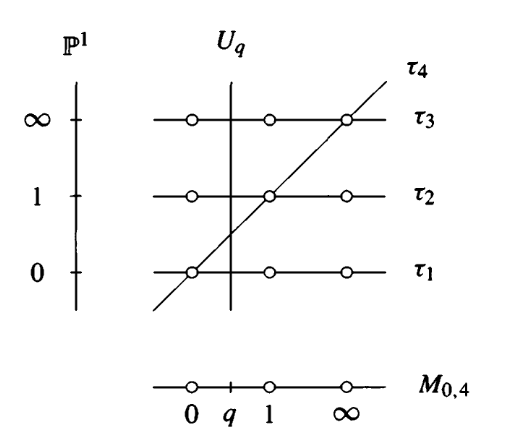
\includegraphics[scale = 0.3]{Chapters/Images/M_04_UniversalFam.png}
    \end{center}
    If we compactify $\mathcal{M}_{0,4}$ to $\mathbb{P}^{1}$ then the sections will no longer be disjoint.
    The diagnoal section $\tau_{4}$ will intersect the other $\tau_{i}'$s at $0,\,1\,\text{and }\infty$ respectively. 
    Therefore, the geometric sections over the points $0,\,1,\, \text{and }\infty$ are $3$-pointed curves, rather than $4$ pointed ones.
    \par To fix this problem we can blow up the universal family $\mathbb{P}^{1} \times \mathbb{P}^{1}$ at the three points, $\tau_{4}\cap \tau_{i}$, for $1\leq i \leq 3$.
    This process of blowing replaces each point $\tau_{4}\cap \tau_{i}$ with a copy of $\mathbb{P}^{1}$ (the exceptional divisor).
    Let $\tilde{\tau}_{i}$ denote the sections to the the blowup of the unversal family, then the fibre over $0$, $U_{0}$, looks like the following.
    \begin{center}
    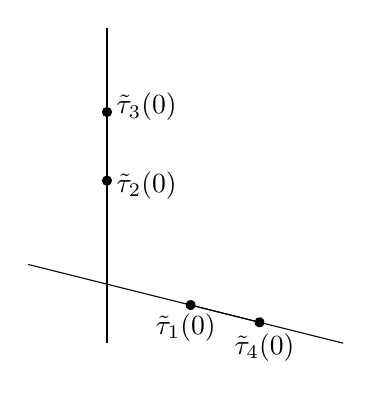
\begin{tikzpicture}
        \draw (1,0) -- (1,4);
        \draw (0,1) -- (4,0);
    \draw[Circle-Circle] (1,3) node[right] {$\tilde{\tau}_{3}(0)$} -- (1,2)node[right] {$\tilde{\tau}_{2}(0)$};
        \draw[Circle-Circle] (2,0.5)node[below] {$\tilde{\tau}_{1}(0)$} -- (3,0.25)node[below] {$\tilde{\tau}_{4}(0)$};
    \end{tikzpicture}    
    \end{center}
    This fibre clearly isn't a smooth variety isomorphic to $\mathbb{P}^{1}$, but it gives us an idea of curves we may want to include in our family if we want our moduli space to be compact. 
    To be specific, we will include reducible curves with some additional structures in our family.
\end{example}
Taking the preceeding example as motivation we introduce the notion of \textit{trees} and \textit{stable curves}.
\begin{definition}
    A \textbf{tree of projective lines} is a connected curve such that:
    \begin{itemize}
        \item All irreducible components are isomorphic to $\mathbb{P}^{1}$.
        \item The points of intersection between irreducible components are ordinary double points (so no intersections are tangential).
        \item There are no closed cricuits, that is, if a node is removed, then the curve becomes disconnected.
    \end{itemize}
    We will refer to these as just trees.
    Further, the irreducible components are called \textbf{twigs}.
\end{definition}
\begin{definition}
    Let $n  \geq 3$. 
    We refer to the marked points and nodes as \textit{special points}.
    A stable $n$-pointed rational curve is a tree $C$ of projective lines, with $n$ distinct marked points (which don't overlap with the nodes) such that each twig has atleast $3$ special points. 
\end{definition}

Notice that the fibres over $0,\,1,\,\infty$ in Example \ref{M04Example} are stable $4$-pointed curves with two twigs.

\begin{remark}
 \par The stability condition in the previous definition is equivalent to saying that curve is automorphism free.
Any automorphism of a $n$-pointed stable curves sends the marked point to itself. 
Therefore, any twig with one node will be sent to itself. 
Since singular points are mapped to singular points, the node must be sent to itself to himself.
By induction it's easy to see that all nodes will mapped to themselves, and consquently, all twigs are sent to itself.
This implies that an automorphism of a stable curve is formed by gluing together automorphisms of the twigs.
But by stability, each twig has more than three special points, each of which is mapped to themselves, implying that their automorphisms are trivial.
Showing that the automorphisms for stable curves are trivial.
\end{remark}
\subsection{Forgetting points, Stabilisation and Contraction}
The addition of reducible curves to our problem gives rise to a few key operations on them.
These operations answer questions regarding what happens to a $n$-pointed curve when we add or remove points from it.
\subsubsection{Stabilisation}
Consider a $n$-marked curve $(C, p_{1}, \dots, p_{n})$.
There are two possibilities for where a $n+1^{\text{th}}$ point can be added.
If the new point doesn't overlap with any of the other special points, the $n+1$ marked tree is a stable curve.
The case which is intersting is when the $n+1^{\text{th}}$ point overlaps one of the special points.

\par We first look at the case where the new point overlaps with a marked point.
\begin{center}
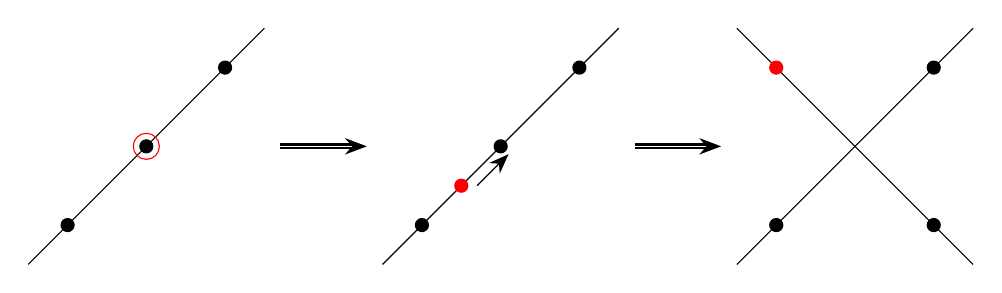
\begin{tikzpicture}
    %First Diagram
    \draw (-7.5,0) -- (-4.5,3);
    \draw (-7,0.5) node [shape=circle, draw = black,fill = black, scale = 0.5]{};
    \draw (-6,1.5) node [shape=circle, draw = black,fill = black, scale = 0.5]{};
    \draw (-5,2.5) node [shape=circle, draw = black,fill = black, scale = 0.5]{};
    \draw (-6,1.5) node [shape=circle, draw = red, scale = 1]{};
    %Second Diagram
    \draw (-3,0) -- (0,3);
    \draw (-2.5,0.5) node [shape=circle, draw = black,fill = black, scale = 0.5]{};
    \draw (-1.5,1.5) node [shape=circle, draw = black,fill = black, scale = 0.5]{};
    \draw (-0.5,2.5) node [shape=circle, draw = black,fill = black, scale = 0.5]{};
    \draw (-2,1) node [shape=circle, draw = red,fill = red, scale = 0.5]{};
    \draw[-{Stealth[scale = 1.5]}] (-1.8,1) -- (-1.4,1.4);
    %Third Diagram
    \draw (1.5,0) -- (4.5,3);
    \draw (2,0.5) node [shape=circle, draw = black,fill = black, scale = 0.5]{};
    \draw (4,2.5) node [shape=circle, draw = black,fill = black, scale = 0.5]{};
    \draw (1.5,3) -- (4.5,0);
    \draw (2,2.5) node [shape=circle, draw = red,fill = red, scale = 0.5]{};
    \draw (4,0.5) node [shape=circle, draw = black,fill = black, scale = 0.5]{};
    %Transitions
    \draw[double, -{Stealth}, thick] (-4.3,1.5) -- (-3.2,1.5);
    \draw[double, -{Stealth}, thick] (0.2,1.5) -- (1.3,1.5);
\end{tikzpicture}
\end{center}
\par The red circle in the left picture on top dentoes the additional point.
We treat this curve as the limit of a family of curves where the a the fourth point approaches the middle point, as shown in the middle picture.
As seen in the earlier example of moduli spaces of $4$-pointed curves, the limit of this family is a reducible curve with twigs, as shown in the right picture. 
The curve on the right is called the \textbf{stabilisation} of the left most curve.
\par Similartly When a new point overlaps a node, we treat it like like a limiting family curves where the new point approaches the node like above.
Then the limit curve formed by a blowup in the universal family gives us the stabilisation.
\par We can also stabilise in families, which is formalised in the next proposition(given without proof).
\begin{proposition}
    For a family $(\mathfrak{X}/B, \sigma_{1},\dots,\sigma_{n})$ of stable $n$-pointed curves, let $\delta$ be an additional section.
    Then there exists a family $(\mathfrak{X}'/B, \sigma'_{1},\dots,\sigma'_{n+1})$ of stable $n+1$-pointed curves and a morphism $\varphi: \mathfrak{X}'\to \mathfrak{X}$ such that:
    \begin{itemize}
        \item The restriction of $\varphi$ on $\varphi^{-1}(\mathfrak{X}\backslash \delta) \to \mathfrak{X}\backslash \delta$ is an isomorphism.
        \item $\varphi \circ \sigma'_{n+1} = \delta$, and $\varphi \circ \sigma'_{i} = \sigma_{i}$ for $i \leq n$.
    \end{itemize}
    This family is unique upto isomorphism, and is called the \textbf{stabilisation} of $(\mathfrak{X}/B, \sigma_{1}, \dots, \sigma_{n})$. Further, stabilisation commutes with fibre products.
\end{proposition}

\subsubsection{Forgetful Maps and Contraction}
We now discuss the converse, how do we forget a marked point of a stable $n$-pointed curve? 
That is, what happens when we go from $(C,p_{1}, \dots,p_{n+1})$ to $(C,p_{1}, \dots,p_{n})$. 
If $p_{n+1}$ lies on a twig with $4$ or more special points, the resulting $n$ pointed curve remains stable, hence the resulting curve is just the same curve with onw less point. 
Problems start occuring when the $n+1^{\text{th}}$ point lies on a twig with $3$ or less special points. 
This has two cases.
\par $1.$ \textit{$p_{n+1}$ lies on a twig with two nodes}.
\begin{center}
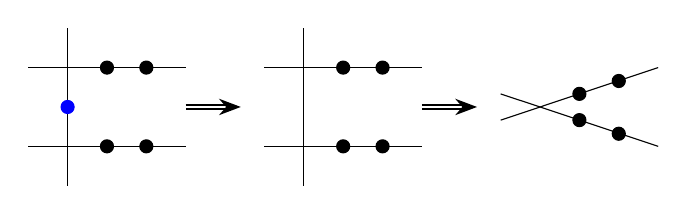
\begin{tikzpicture}
    %First
    \draw (-4.5,0) -- (-4.5,2);
    \draw (-5,0.5) -- (-3,0.5);
    \draw (-5, 1.5) -- (-3,1.5);
    \draw (-4.5,1) node [shape=circle, draw = blue,fill = blue, scale = 0.5]{};
    \draw (-3.5,1.5) node [shape=circle, draw = black,fill = black, scale = 0.5]{};
    \draw (-4,1.5) node [shape=circle, draw = black,fill = black, scale = 0.5]{};
    \draw (-3.5,0.5) node [shape=circle, draw = black,fill = black, scale = 0.5]{};
    \draw (-4,0.5) node [shape=circle, draw = black,fill = black, scale = 0.5]{};
    %Second
    \draw (-1.5,0) -- (-1.5,2);
    \draw (-2,0.5) -- (0,0.5);
    \draw (-2, 1.5) -- (0,1.5);
    \draw (-0.5,1.5) node [shape=circle, draw = black,fill = black, scale = 0.5]{};
    \draw (-1,1.5) node [shape=circle, draw = black,fill = black, scale = 0.5]{};
    \draw (-0.5,0.5) node [shape=circle, draw = black,fill = black, scale = 0.5]{};
    \draw (-1,0.5) node [shape=circle, draw = black,fill = black, scale = 0.5]{};
    %Third
    \draw (1,0.833) -- (3,1.5);
    \draw (1, 1.166) -- (3,0.5);
    \draw (2.5,1.33) node [shape=circle, draw = black,fill = black, scale = 0.5]{};
    \draw (2,1.1666) node [shape=circle, draw = black,fill = black, scale = 0.5]{};
    \draw (2.5,0.66) node [shape=circle, draw = black,fill = black, scale = 0.5]{};
    \draw (2,0.833) node [shape=circle, draw = black,fill = black, scale = 0.5]{};
%    \draw (1.5,1) node [shape=circle, draw = black, scale = 0.5];
    %transitions
    \draw[double, -{Stealth}, thick] (-3,1) -- (-2.3,1);
    \draw[double, -{Stealth}, thick] (0,1) -- (0.7,1);
\end{tikzpicture}
\end{center}
When we remove a point a on a twig with two other nodes we contract the twig to a single point, resulting in the two adjacent twigs intersecting with each other, like in the diagram above.
So this is a two step proccess, \textbf{forgetting} followed by \textbf{contraction}. 
\par $2.$ \textit{$p_{n+1}$ lies on a twig with a node and a marked point}.
\begin{center}
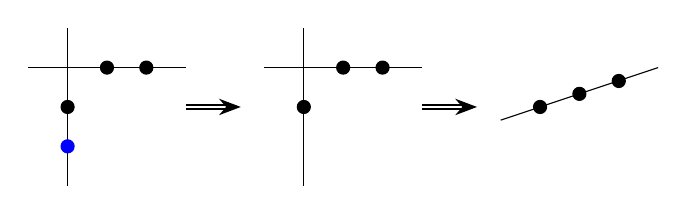
\begin{tikzpicture}
    %First
    \draw (-4.5,0) -- (-4.5,2);
    \draw (-5, 1.5) -- (-3,1.5);
    \draw (-4.5,0.5) node [shape=circle, draw = blue,fill = blue, scale = 0.5]{};
    \draw (-4.5,1) node [shape=circle, draw = black,fill = black, scale = 0.5]{};
    \draw (-3.5,1.5) node [shape=circle, draw = black,fill = black, scale = 0.5]{};
    \draw (-4,1.5) node [shape=circle, draw = black,fill = black, scale = 0.5]{};
    %Second
    \draw (-1.5,0) -- (-1.5,2);
    \draw (-2, 1.5) -- (0,1.5);
    \draw (-1.5,1) node [shape=circle, draw = black,fill = black, scale = 0.5]{};
    \draw (-0.5,1.5) node [shape=circle, draw = black,fill = black, scale = 0.5]{};
    \draw (-1,1.5) node [shape=circle, draw = black,fill = black, scale = 0.5]{};
    %Third
    \draw (1,0.833) -- (3,1.5);
    \draw (1.5,1) node [shape=circle, draw = black, fill = black, scale = 0.5]{};
    \draw (2.5,1.33) node [shape=circle, draw = black,fill = black, scale = 0.5]{};
    \draw (2,1.1666) node [shape=circle, draw = black,fill = black, scale = 0.5]{};
    %transitions
    \draw[double, -{Stealth}, thick] (-3,1) -- (-2.3,1);
    \draw[double, -{Stealth}, thick] (0,1) -- (0.7,1);
\end{tikzpicture}
\end{center}
\par Here again, after the marked point is removed, we contract the unstable twig.
The key difference here is that the point of intersection with the other twig becomes a marked point after contraction.
This again can be formalised for familes, as we do in the next proposition without proof.
\begin{proposition}
    For a family $(\mathfrak{X}'/B, \sigma'_{1},\dots, \sigma'_{n+1})$ of stable $n+1$-pointed curves there exists a family $(\mathfrak{X}/B, \sigma_{1},\dots, \sigma_{n})$ and $B$-morphism $\varphi: \mathfrak{X}' \to \mathfrak{X}$ such that:
    \begin{itemize}
        \item $\varphi \circ \sigma' = \sigma$ for $1\leq i \leq n$.
        \item for each $b \in B$ the morphism at the level of fibres $\mathfrak{X}'_{b}\to \mathfrak{X}_{b}$ is an isomorphism when restricted to any stable twig of $(\mathfrak{X}'_{b}, \sigma'_{1}(b), \dots, \sigma'_{n}(b))$.
    \end{itemize}
    This family is unique upto isomorphism, and we shall is say that it is obtained from $\mathfrak{X}'/B$ by forgetting the section $\sigma'_{n+1}$. Further, forgetting commutes with fibre products.
\end{proposition}

When we forget the last section for the universal family over $n+1$ points, we get a family of $n$-points over $\overline{\mathcal{M}}_{0,n+1}$. 
Via the universal propery of $\overline{U}_{0,n}/\overline{\mathcal{M}}_{0,n}$ there exists a unique morphism:
\begin{align*}
    \varepsilon : \overline{\mathcal{M}}_{0,n+1} \to \overline{\mathcal{M}}_{0,n},
\end{align*}
which we call the \textbf{forgetful map}.
 
\subsection{$\mathcal{M}_{0,n}$ and Boundary Divisors}

\subsubsection{A Set Theoretic bijection between $\overline{\mathcal{M}}_{0,n+1}$ and $\overline{U}_{0,n}$}
We understand the bijection between $\overline{\mathcal{M}}_{0,n+1}$ and $\overline{U}_{0,n}$ by examining the $n=4$ case.
Consider a point $p \in \overline{U}_{0,4}$; to this point we are going to assign a stable $5$-pointed curve $C_{p}$.
Let $F_{p}$ denote the $4$-pointed curve $\pi^{-1}(\pi(p))$ where $\pi: \overline{U}_{4} \to \overline{\mathcal{M}}_{0,4}$.
Then $p$ lies on the curve $F_{q}$; if $p$ doesn't overlap with any of the special points, then define $C_{p} := (F_{p},p)$, else if $p$ overlaps with a special point define $C_{p}$ to be the stabilisation of $(F_{p},p)$.
If we interpret $C_{p}$ as it's corresponding point in $\overline{\mathcal{M}}_{0,5}$ we have established an \textit{injective} map $\overline{U}_{0,4} \to \overline{\mathcal{M}}_{0,5}$.
\par It's easy to check the srujectivity of this map.
Consider a $5$-pointed curve $(C,p_{1},\dots, p_{5})$, let $F_{q}$ be the four pointed curve obtained by forgetting the last point (contracting, if required).
That is, the $4$-pointed curve corresponding to the image of the curve under the forgetful map $\varepsilon : \overline{\mathcal{M}}_{0,5}\to \overline{\mathcal{M}}_{0,4}$.
To obtain a point in the universal family $\overline{U}_{0,4}$, we consider the fibre over the point in $\overline{\mathcal{M}}_{0,4}$ and choose the point to be the image of $p_{5}$ under forgetting and contracting. 
It's easy to see that this is an inverse to the previous map, and hence a bijection between $\overline{\mathcal{M}}_{0,5}$ and $\overline{U}_{0,4}$.
\par This set-theoretic bijection is also an isomorphism of schemes.

\subsubsection{Construction of the Universal Family $\overline{U}_{0,5}$}
Now that we have shown $\overline{\mathcal{M}}_{0,n+1}$ and $\overline{U}_{0,4}$ are isomorphic, to construct $\overline{\mathcal{M}}_{0,n}$ for any $n$ we need to see how to obtain the universal family from the moduli space.
We draw inspiration from the $n=4$ case and look at the fibre products of $\overline{\mathcal{M}}_{0,5}$ with itself over the base scheme $\overline{\mathcal{M}}_{0,4}$.
Let $\overline{\mathfrak{U}}_{0,5}$ denote the stabilisation of $\overline{\mathcal{M}}_{0,5} \times_{\overline{\mathcal{M}}_{0,4}} \overline{\mathcal{M}}_{0,5}$, over the base $\overline{\mathcal{M}}_{0,5}$. 
We then have the following diagram.
\[
\begin{tikzcd}
    \overline{\mathfrak{U}}_{0,5} & & \\
    \\
    \overline{U}_{0,4} \times_{\overline{\mathcal{M}}_{0,4}} \overline{U}_{0,4} & & \overline{\mathcal{M}}_{0,5} \simeq \overline{U}_{0,4} \\
    \\
    \overline{\mathcal{M}}_{0,5} \simeq \overline{U}_{0,4} & & \overline{\mathcal{M}}_{0,4}
    \arrow[from = 1-1, to = 3-1]
    \arrow[from = 3-1, to = 3-3]
    \arrow[from = 3-1, to = 5-1, xshift = -1ex]
    \arrow[from = 5-1, to = 5-3]
    \arrow[from = 3-3, to = 5-3, xshift = -1ex]
    % sections
    \arrow[from = 5-1, to = 3-1, xshift = 1.3ex]
    \arrow[from = 5-1, to = 3-1, xshift = 2.6ex]
    \arrow[from = 5-1, to = 3-1, xshift = 3.9ex]
    \arrow[swap, "\sigma_{i}",from = 5-1, to = 3-1, xshift = 5.2ex]
    \arrow["\delta", from = 5-1, to = 3-1, xshift = -3ex]
    %more sections
    \arrow[from = 5-3, to = 3-3, xshift = 1.3ex]
    \arrow[from = 5-3, to = 3-3, xshift = 2.6ex]
    \arrow[from = 5-3, to = 3-3, xshift = 3.9ex]
    \arrow[swap, "\sigma_{i}",from = 5-3, to = 3-3, xshift = 5.2ex]
\end{tikzcd}
\]
By using commutativity of stabilisation with fibred products it's easy to show that this stabilisation $\overline{\mathfrak{U}}_{0,5}$ is the universal family over $\overline{\mathcal{M}}_{0,5}$.
And hence $\overline{U}_{0,5}:=\overline{\mathfrak{U}}_{0,5}$.
\subsubsection{Boundary Divisors}

By the boundary of $\overline{\mathcal{M}}_{0,n}$ we mean the set $\overline{\mathcal{M}}_{0,n} \backslash \mathcal{M}_{0,n}$.
The points of the boundary correspond to reducible curves.
In this section we will classify the set of reducible curves, and discuss the properties of the set of reducible curves of codimension $1$.

\begin{proposition}
    The the subset $\Sigma_{\delta} \subset \overline{\mathcal{M}}_{0,n}$ consisting of curves with $\delta \leq n-3$ number of nodes is of \textit{pure} dimension $n-3-\delta$.
\end{proposition}
\begin{proof}
    hm.
\end{proof}

\begin{definition}[Ordered Partition]
    Let $S$ be a set with $|S| = n < \infty$.
    A partition of $S$ is a set of disjoint subsets $\{A_{i}\}_{i=0}^{r}$ such that $\bigcap_{i=0}^{r}A_{i} = S$.
    On each element $A_{i}$ we can define an ordering of its elements given by $<_{i}$ (usually this ordering is given by the ordering of points in the set $S$).
    We refer to the partition along with the ordering, $\{(A_{i},<_{i}): 0 \leq i\leq r\}$, as a \textbf{ordered partition}.
    We will call an ordered partition stable if $|A_{i}|\geq 2$ for all $i$.
\end{definition}

\begin{definition}[Labeled Configuration]
    Consider the set $S = \{p_{1}, \dots, p_{n}\}$ of marked points for the moduli space $\overline{\mathcal{M}}_{0,n}$. 
    Over each stable ordered partition, $\mathcal{A}$, of the set $S$ we can construct a set of $n$-marked curves:
    \begin{itemize}
        \item Let the ordered partition be $\{(A_{i},<_{i}): 0 \leq i\leq r\}$.
        \item Consider a tree $C$ with $r$ nodes.
        \item Since a tree is connected with no cycles, there exist $r+1$ twigs in $C$.
        \item Label the twigs $T_{i}$ for $0\leq i \leq r$, such that for all $i$, the intersection $T_{i}\cap T_{i+1} \neq \emptyset$. 
            It's easy to see that there exist only two such sequences, $T_{i}$ and $T_{r-i}$.
        \item To each twig $T_{i}$ assign $|A_{i}|$ marked points, and label them with respect to the ordering $<_{i}$ - making $C$ a $n$-marked curve.
        \item Let $F_{\mathcal{A}}$ denote the set of all these $n$-marked curves upto automorphisms (preserving the ordered partitioning).
    \end{itemize}
    The set $F_{\mathcal{A}}$ is called a \textbf{labeled configuration}.
\end{definition}

%\begin{example}
%    \textcolor{red}{[Add example of a labeled configuration]}
%\end{example}

\begin{definition}
    The closure of each labeled configuration is a smooth and irreducible subvariety of $\overline{\mathcal{M}}_{0,n}$, called a \textbf{boundary cycle}.
    \par The boundary of boundary cycles are made from other boundary cycles of higher codimension (more elements in the ordered parition).
\end{definition}

\begin{remark}
    Since the set $S = \{p_{1}, \dots, p_{n}\}$ we partition to define cycles already has an ordering, from now on we will assume that the ordering on the partitions is induced from this ordering. Hence we choose to drop the term \textit{ordered} while referring to partitions.
\end{remark}

\begin{definition}[Boundary Divisors]
    Boundary cycles of codimension $1$ are called \textbf{boundary divisors}. 
    They are the closure of a labeled configuration $T_{\mathcal{A}}$, where $\mathcal{A}$ is a stable partition with two elements.
    For a stable partition $S = A \cup B$ of the marked points, the divisor defined by the induced labeled configuration is denoted as $D(A|B)$.
    \par A general point of the divisor $D(A|B)$ is a curve with two twigs, such that the set of marks $A$ and $B$ are distributed among different twigs.
\end{definition}

%\begin{example}
%    \textcolor{red}{[Add an example for divisors]}
%\end{example}

\begin{proposition}[The recursive structure of divisors]
    Each boundary cycle can be expressed as a finite product of moduli spaces of lower dimension. 
    In paritcular, a divisor $D(A|B)$ is isomorphic to $\overline{\mathcal{M}}_{0,A \cup \{x\}} \times \overline{\mathcal{M}}_{0,B \cup \{x\}}$.
\par We will just discuss the idea behind the proof for the case of divisors and leave it to the reader to extend the ideas to the case of boundary cycles.
\end{proposition}
%\begin{proof}[Sketch of a proof]
%    \textcolor{red}{fill this}
%\end{proof}

%\begin{remark}
%    On compatibility of forgetful maps with the recursive structures of divisors. \textcolor{red}{Talk to vivek and fix this}.
%\end{remark}

%\textcolor{red}{[Primitive version of WDVV equations]}

\section{Stable Maps}

%\textcolor{red}{[Rewrite this paragraph later]}
Over this section we will define and understand the properties of moduli spaces of stable maps $\overline{\mathcal{M}}_{0,n}(\mathbb{P}^{r},d)$.
Since the goal of this chapter is to study the intersections of degree $d$ curves in projective space, these moduli spaces will serve as an important tool.

\begin{definition}
    A family of maps of smooth raional curves is a diagram
    \[
        \begin{tikzcd}
            \mathfrak{X} & & \mathbb{P}^{r}\\
            \\
            B
            \arrow["\mu", from = 1-1, to = 1-3]
            \arrow["\pi", from = 1-1, to = 3-1]
        \end{tikzcd}
    \]
    where $\pi$ is a flat family with geometric fibres isomorphic to $\mathbb{P}^{1}$.
    The map $\mu$ restriced to the fibres $\mathfrak{X}_{b}$ of points $b \in B$, denoted $\mu_{b}$, is a map from a smooth eational curve. 
    Futher, it can be shown that all fibres $\mu_{b}$ have the same degree.
\end{definition}

\subsection{Moduli Spaces of maps to $\mathbb{P}^{r}$}

\subsubsection{The Space of Parameterisations}

\begin{definition}[Degree of a map]
    The degree of the map $\mu : \mathbb{P}^{1} \to \mathbb{P}^{r}$ is defined as the degree of the direct image cycle $\mu_{*}[\mathbb{P}^{1}]$.
    That is, if $e$ is degree of the image curve, and $k$ the degree of the field extension corresponding to the map $\mu$, then the degree is defined to be $k \cdot e$.
\end{definition}

An easier way to understand this notion of degree is by looking at the explicit form of the morphism $\mu$.
$\mu$ is of the form $\mu([x;y]) = [F_{0}(x,y);\cdots ; F_{r}(x,y)]$ where $F_{i}$'s are homogenous polynomials, then $\text{deg}(\mu) = \text{deg}(F_{i})$ for any $0 \leq i \leq r$. 
This characterisation makes sense since all $F_{i}$'s are homogenous.
This interpretation of $\mu$ also helps us define thee space of degree $d$ maps $\mathbb{P}^{1} \to \mathbb{P}^{r}$.
Note that each degree $d$ map $\mathbb{P}^{1} \to \mathbb{P}^{r}$ is a parameterisation of the image curve, hence we refer to the set of all such maps as the \textit{space of parametrisations}, and denote it $W(r,d)$. 

\par Defining a map $\mu : \mathbb{P}^{1} \to \mathbb{P}^{r}$ of degree $d$ is equivalent to defining $r+1$ degree $d$ forms, upto a constant factor.
This condition characterises $W(r,d)$ as a Zariski open subset:
\begin{align*}
    W(r,d) \subset \mathbb{P}\left(\bigoplus_{i=0}^{r}H^{0}(\mathcal{O}_{\mathbb{P}^{1}}(d)) \right).
\end{align*}
Here $H^{0}(\mathcal{O}_{\mathbb{P}^{1}}(d))$ is the set of global sections on $\mathbb{P}^{1}$ of degree $d$.
The dimension of $W(r,d)$ is $1$ less than the dimension of the space with $r+1$ degree $d$ forms since we are going modulo a constant factor, 
\begin{align*}
    \text{dim}(W(r,d)) = (r+1)(d+1) - 1 = rd + r + d.
\end{align*}
\par $W(r,d)$ admits a canonical family of maps $\mathbb{P}^{1} \to \mathbb{P}^{r}$.
For the family given by the projection $\pi : W(r,d) \times \mathbb{P}^{1} \to W(r,d)$, the fibre over each morphism $\mu \in W(r,d)$ is mapped to curve $\mu(\mathbb{P}^{1}) \subset \mathbb{P}^{r}$.
It turns out that this canonical family is the universal family of the moduli space for maps $\mathbb{P}^{1} \to \mathbb{P}^{r}$ of degree $d$.
\begin{definition}
    A map $\mu :\mathbb{P}^{1} \to \mathbb{P}^{r}$ is called an \textbf{immersion} when the induced tangent map is injective at all points.
\end{definition}
\begin{lemma}[On Codimension of Space of Parametrisations]
    The set $W^{\circ}(r,d) \subset W(r,d)$ of all immersions is \textit{open}.
    For $d=1$, $W^{\circ}(r,1)  = W(r,1)$. For $d\geq 2$, its complement is of codimension $r-1$.
\end{lemma}
%\begin{proof}
%    \textcolor{red}{[May add it later]}
%\end{proof}

An important subset of $W(r,d)$ is the maps which are birational onto their image, we denote this subset with $W^{*}(r,d)$.
Just like in the previous lemma, we will now try to find a bound on the codimension of the complement of $W^{*}(r,d)$. 
We there for ask, what does the complement of $W^{*}(r,d)$ look like?
For $d=1$ this is trivial since $W^{\circ}(r,1) = W^{*}(r,1) =  W(r,1)$.
dotted arrow latex
\par Before, examining the $d \geq 2$ case, recall the following proposition.
\begin{proposition}
    %[\textcolor{red}{Cite 7.16 from Harris}]
    Let $f: X \dashrightarrow Y$ be a dominant rational map between two varieties. 
    The general fibre of the map $f$ is finite \textbf{iff} the map $f^{*}: K(Y) \to K(X)$ is a finite field extension.
    Further, when the base field $K$ is of characteristic $0$, the degree of the map is equal to the cardinality of the general fibre.
\end{proposition}

Returning to the $d \geq 2$ case, since the map $\mu$ in discussion is not birational the cardinality of the general fibre is atleast $2$.
Consequently, from the above lemma, the degree of the field extension corresponding to the map is of atleast degree $2$.
We refer to maps of this kind as \textit{multiple covers}.
\par Every multiple cover $\mu: \mathbb{P}^{1} \to \mathbb{P}^{r}$ factors via $\mathbb{P}^{1}$ as $\mathbb{P}^{1} \xrightarrow{\rho} \mathbb{P}^{1} \xrightarrow{\psi} \mathbb{P}^{n} $, where $\rho$ is a multiple cover of the projective line, and $\psi$ a map birational onto its image.
This factorisation is not unique since for every automorphism $\phi$ of $\mathbb{P}^{1}$ we have a factorisation $(\psi \circ \phi^{-1}) \circ (\phi \circ \rho)$. 
Remember that the degree $d$ of $\mu$ is defined as $d = ke$, where $e$ is the degree of the image curve and $k$ the degree of the associated field extension.
In the above factorisation of $\mu$, $\rho$ is a $k$-fold cover of $\mathbb{P}^{1}$, and the image of $\psi$ is a degree $e$ curve in $\mathbb{P}^{r}$.
\par This gives a relation between factorisations of $d$ and factorisations of $\mu$ via $\mathbb{P}^{1}$. 
To establish a bound on the codimension of the complement of $W^{*}(r,d)$, we study the locus of maps associated with each factorisation of $d$ in the complement.
In particular, we are looking for factorisations where the associated locus achieves the least possible codimension.

%\begin{lemma}[generalisation of Lemma 2.1.4 and 2.1.5 from Kock's book]
%    \textcolor{red}{Prove this lemma in notes and write it here}
%\end{lemma}

\begin{proposition}
    The locus $W^{*}(r,d) \subset W(r,d)$ is open, and for $d \geq 2$ the codimension of its complement is atleast:
    \begin{align*}
        \text{min}\{(r-1)(d-1),(r+1)d/2 - 2\}.
    \end{align*}
    For $r \geq 2$ this locus is dense in $W(r,d)$.
\end{proposition}

%begin{lemma}
%   The locus in $W(r,d)$ of $d$-fold covers of a line is closed, with codimension $(r-1)(d-1)$.
%end{lemma}
%
%begin{lemma}
%   Suppose $d$ is even. Then the closure of the locus of double covers of curves of degree $d/2$ is of codimension $(r+1)d/2 - 2$.
%\end{lemma}

\subsubsection{Problems with this space of Parametrisations}
We now see why the space $W(r,d)$ is not good enough:
\begin{itemize}
    \item The families assosciated with $W(r,d)$ are such that all parametrisations are induced from the same $\mathbb{P}^{1}$, but we will see in a following example 
        %\textcolor{red}{[add example]} 
        that there exists families of rational curves where maps come from different $\mathbb{P}^{1}$.
    \item The space $W(r,d)$ isn't compact, which makes it hard to define a good intersection theory on it.
    \item Additionaly, reparametrisations of the same family are considered as different elements of the moduli space.
\end{itemize}

\begin{example}
    Consider the rational map $\mu: \mathbb{P}^{2} \dashrightarrow \mathbb{P}^{1}$ given by the projection $[x;y;z] \to [x;y]$. 
    We resolve this map by considering the blowup of $\mu$.
    Since the locus $V(x,y) = \{[0;0;1]\}$ in $\mathbb{P}^{2}$, the map $\mu$ can be interpreted as projection along the point $[0;0;1]$.
    Let $\tilde{\mathbb{P}}^{2}$ denote the closure of the graph of $\mu$ in $\mathbb{P}^{2} \times \mathbb{P}^{1}$.
   % \par \textcolor{red}{Finish this example after working out the blow-up thing}
\end{example}
\par To remedy the third drawback in the above discussion, we give the quotient $W(r,d)/\text{Aut}\mathbb{P}^{1}$ the structure of a variety.
The following lemma hints at the likelyhood for the existence of a coarse moduli space.

\begin{lemma}
    Let $\mu : \mathbb{P}^{1} \to \mathbb{P}^{r}$ be a non-constant map. 
    Then there exists only a finite number of automophisms $\phi$ of $\mathbb{P}^{1}$ such that $\mu = \mu \circ \phi$.
    If $\mu$ is birational onto its image, $\text{Aut}(\mu)$ is trivial.
\end{lemma}

Notice that a consquence of the previous lemma is that the open set $W^{*}(r,d) \subset W(r,d)$ is precisely the set of automorphism free maps - since maps are birational onto their image if and only if the field extension is of degree $1$. 
The set, 
\begin{align*}
    \mathcal{M}^{*}_{0,0}(\mathbb{P}^{r},d) \simeq W^{*}(r,d)/\text{Aut}(\mathbb{P}^{1})
\end{align*}
is the fine moduli space for the family of autmorphism free maps into $\mathbb{P}^{r}$.
\par Further, when $d \geq 1$ the maps in the complement of $W^{*}(r,d)$ are the \textit{multiple cover} maps discussed earlier. 
When we take these maps into account, we get the \textit{coarse moduli space}:
\begin{align*}
    \mathcal{M}_{0,0}(\mathbb{P}^{r},d) \simeq W(r,d)/\text{Aut}(\mathbb{P}^{1}).
\end{align*}
The dimension, $\text{dim}\mathcal{M}_{0,0}(\mathbb{P}^{r},d) = rd + r + d -3$.
Notice when $r\geq 2$ and $d \geq 1$, 
%from \textcolor{red}{Cite Lemma} 
it follows that $\mathcal{M}^{*}_{0,0}(\mathbb{P}^{r},d)$ is dense in $\mathcal{M}^{*}_{0,0}(\mathbb{P}^{r},d)$.


\begin{proposition}
    For $n \geq 3$ there exists a fine moduli space $\mathcal{M}_{0,n}(\mathbb{P}^{r},d)$ for isomorphism classes of $n$- pointed maps of degree $d$,
    \begin{align*}
        \mathcal{M}_{0,n}(\mathbb{P}^{r},d) = \mathcal{M}_{0,n} \times W(r,d).
    \end{align*}
    In fact, $\mathcal{M}_{0,n}(\mathbb{P}^{r},d)$ is a smooth variety.
\end{proposition}

%\subsubsection{Example: Degree 1 Maps}
%\textcolor{red}{[May Add]}
\subsection{Kontsevich Stable Maps}

%\subsubsection{Examples motivating the definition}
%\textcolor{red}{[Unsure if I want to add this section] - will see on based on length of rest of this chapter.}

\subsubsection{The space of Stable Maps}
We now introduce the notion of \textit{Kontsevich Stable Maps}.
Just like how we defined the notion of stability for $n$-marked curves, we will define a similar notion of stability for maps into $\mathbb{P}^{r}$.
\begin{definition}[$n$-pointed maps]
    An $n$-pointed map is a morphism $\mu : C \to \mathbb{P}^{r}$, where $C$ denotes a tree of projective lines with $n$ distinct marked smooth points of $C$.
    An isomorphism of $n$-pointed maps, $\mu : C \to \mathbb{P}^{r}$ and $\mu' : C' \to \mathbb{P}^{r}$ is a morphism $\phi : C \to C'$ such that following diagrams commute:
\[
    \begin{tikzcd}
        C & & C' & & C & & C' \\
        \\
        \emph{Spec}\mathbb{C} & & \emph{Spec}\mathbb{C} & & & \mathbb{P}^{r} & 
        \arrow["\phi", from = 1-1, to = 1-3]
        \arrow["\phi", from = 1-5, to = 1-7]
        \arrow[swap,"\mu", from = 1-5, to = 3-6]
        \arrow["\mu'", from = 1-7, to = 3-6]
        \arrow[swap,"\pi", from = 1-1, to = 3-1, xshift = -1ex]
        \arrow[swap,"\pi'", from = 1-3, to = 3-3, xshift = -1ex]
        \arrow[equal, from = 3-1, to = 3-3]
        \arrow[swap,"\sigma_{i}", from = 3-1, to = 1-1, xshift = 1ex]
        \arrow[swap,"\sigma'_{i}", from = 3-3, to = 1-3, xshift = 1ex]
    \end{tikzcd}
\]
\end{definition}
A family of $n$-pointed maps can be understood as the diagram,
\[
    \begin{tikzcd}
        \mathfrak{X} & & \mathbb{P}^{r}\\
        \\
        B & &
        \arrow["\mu", from = 1-1, to = 1-3]
        \arrow[swap, "\pi", from = 1-1, to = 3-1, xshift = -1ex]
        \arrow[swap, "\sigma_{i}", from = 3-1, to = 1-1, xshift = 1ex]
    \end{tikzcd}
\]
where $\pi$ is a flat family of trees, and $\sigma_{i}$ are $n$ disjoint sections which don't intersect the singularities (nodes) of the fibres.
\begin{definition}
    An $n$-pointed map $\mu : C \to \mathbb{P}^{r}$ is called \textit{Kontsevich Stable} if any twig mapped to a point is a stable pointed curve.
\end{definition}
\begin{lemma}[Equivalence of Stability and Cardinality of Automorphism Group]
    An $n$-pointed map is Kontsevich stable if and only if it has a finite number of automorphisms.
\end{lemma}
%\begin{proof}
%    \textcolor{red}{Add this proof later}
%\end{proof}

\par We now state the existence theorem for Kontsevich moduli spaces, without proof.

\begin{theorem}
    \label{stableExistTh}
    There exists a coarse modulis space $\overline{\mathcal{M}}_{0,n}(\mathbb{P}^{r},d)$ parametrising isomorphism classes of Kontsevich stable maps of degree $d$.
\end{theorem}

\begin{theorem}
    $\overline{\mathcal{M}}_{0,n}(\mathbb{P}^{r},d)$ is a projective normal irreducible variety, and it is locally ismorphic to a quotient of a smooth varity by the action of a finite group.
    It contains $\overline{\mathcal{M}}^{*}_{0,n}(\mathbb{P}^{r},d)$ as aa smooth open dense subvariety which is a fine moduli space for maps without automorphisms.
\end{theorem}
\begin{remark}
    Since each marked point adds one to the dimension:
    \begin{align*}
        \text{dim}\,\overline{\mathcal{M}}_{0,n}(\mathbb{P}^{r},d) &= (r+1)(d+1) - 1 - 3 +n\\
                                                                 &= rd + r + d + n - 3.
    \end{align*}
\end{remark}
\subsubsection{Idea behind the construction of $\overline{\mathcal{M}}_{0,n}(\mathbb{P}^{r},d)$}
Although we did state the existence of the mouduli space of stable maps in theorem \ref{stableExistTh} we would like to know how this space behaves.
We will now look at the case of stable maps into $\mathbb{P}^{2}$ and discuss some of its properties.
We describe a class of open sets of $\overline{\mathcal{M}}_{0,n}(\mathbb{P}^{2},d)$ which cover the entire space.

\par Fix lines $l_{0},\,l_{1},\,l_{2}$ in $\mathbb{P}^{2}$, defined by the linear forms $x_{0},\, x_{1},\, x_{2} \in H^{0}(\mathcal{O}_{\mathbb{P}^{2}}(1))$.
The open, $U$, set we are interested is the set given by maps in $\overline{\mathcal{M}}_{0,n}(\mathbb{P}^{2},d)$ such that their images intersect transversaly with the lines $l_{i}$.
This is equivalent to saying that the inverse image of the divisor $l_{0}+l_{1}+l_{2}$ consists of $3d$ distinct non-special points of $C$.
The inverse image of this divisor is equally distributed among twigs of $C$.
Remember that the degree of a curve can also be defined by the number of intersection of the curve with a transverse hyperplane divisor. 
Since each $l_{i}$ is a hyperplane divisor in $\mathbb{P}^{2}$, if the restriction of $\mu$ onto a twig is of degree $d'$ then the inverse image divisor $\mu^{*}l_{j}$ has $d'$ points on this twig.
We denote with $D_{j}:= \mu^{*}l_{j}$ the inverse image divisor, and with $q_{j1}, \dots, q_{jd}$the points of $D_{j}$. It's also easy to see that the divisors $D_{j}$ are linearly equivalent, since they come from the sections $\mu^{*}x_{i}$ of the line bundle $\mu^{*}\mathcal{O}_{\mathbb{P}^{2}}(1)$.

\begin{remark}
    In the previous paragraph we assigned to each map $\mu: C \to \mathbb{P}^{2}$ (which were transversal to three linearly equivalent divisors) a $(n+3d)$-point curve $\tilde{C}$. It turns out that this curve $\tilde{C}$ is a $(n+3d)$-pointed stable curve if and only if $\mu:C \to \mathbb{P}^{2}$ is a stable map. 
    We formalise this in the next proposition.
\end{remark}
\begin{proposition}
        For a map $\mu:C \to \mathbb{P}^{2}$ the constructed $(n+3d)$-pointed curve is stable if and only if the map $\mu$ is stable.
\end{proposition}
\begin{proof}
    \par \textit{Suppose $\mu$ is Kontsevitch stable}.
    \par Then by defininition, the degree $0$ twigs (where restriction of $\mu$ is of degree $0$) of $\tilde C$ are already stable.
    As for the twigs with degree $d' \geq 1$, there exist atleast $3d'\geq 3$ marked points on them - hence satisfying the stability condition for pointed curves.
    \par \textit{Suppose $\tilde C$ is a stable $(n+3d)$-pointed curve}.
    \par We go about this via contradiction, say $\mu$ was not kontsevitch stable - there would exist a twig of degree $0$ with less that $3$ special points.
    Consequently the curve $C$ wouldn't be stable as a pointed curve.
    This degree zero twig will remain unstable even we add the $3d$ marked points to construct $\tilde C$ - since all these points are added to twigs with nonzero degree.
    This contradicts that $\tilde C$ is a stable pointed curve - hence $\mu$ is Kontsevich stable.
\end{proof} 

\begin{proposition}
    Let $\tilde{C}$ with marks $p_{1},\allowbreak \dots,\allowbreak p_{n},\allowbreak q_{01},\allowbreak \dots,\allowbreak q_{0d} ,\allowbreak q_{11},\allowbreak \dots,\allowbreak q_{1d},\allowbreak q_{21},\allowbreak \dots,\allowbreak q_{2d}$ be a stable curve.
    Define divisors $D_{j}:= \sum q_{jk}$.
    If the divisors are \textit{linearly equivalent} there exists an element $\mu \in \overline{\mathcal{M}}_{0,n}(\mathbb{P}^{2},d)$ such that the $(n+3d)$-curve constructed by the inverse image divisors of $\sum_{i}l_{i}$ is $\tilde{C}$.
\end{proposition}
\begin{proof}
    Since the divisors $D_{j}$ are linearly equivalent, they arise from sections of the same line bundle, say $\mathcal{O}(D)$.
    Let $\tilde{s}_{0},\, \tilde{s}_{1},\,\tilde{s}_{2}$ be the sections which give rise to $D_{0},\,D_{1},\,D_{2}$ respectively.
    Since these sections are disjoint, they define a morphism $\tilde{\mu}: \tilde C \to \mathbb{P}^{2}$ given by $x \mapsto [\tilde{s}_{0}(x);\tilde{s}_{1}(x);\tilde{s}_{2}(x)]$.
    We can choose a $\phi \in \text{Aut}(\mathbb{P}^{2})$ such that $(\phi \circ \tilde{\mu})^{*}l_{i} = \tilde{s}_{i}$ for the divisors $l_{i}$ defined by the linear forms $x_{i}$.
    If we now forget the $3d$ marked points and let $\mu := \phi \circ \mu$ be a map from $C$, the curve with $n$-marked points, then the $n+3d$-pointed curve induced by $\mu$ is same as the $\tilde{C}$ we started off with.
    Hence we are done.
\end{proof}

\begin{remark}
    We define $B \subset \overline{\mathcal{M}}_{0,n+3d}$ to be the set of pointed curves such that divisors $D_{j}$ (defined in the above proposition) are linearly equivalent. 
    A condition for $(\tilde C, (p_{i}), (q_{jk})) \in \overline{\mathcal{M}}_{0,n+3d}$ to lie in $B$ equivalent to the linear equivalence of divisors is that the number of points of the divisor $D_{j}$ lying on a twig is independent of $j$; that is, each divisor contributes the same number of points on a twig.
    It follows that the complement of $B$ consists of boundary divisors $D(A|A')$ such that $A$ intersects $D_{j}$ at more points than $A'$. Implying, $B$ is a \textit{open subset} in $\overline{\mathcal{M}}_{0,n+3d}$.
    Further, $B$ also clearly contains all the irreducible $n+3d$ pointed curves in $\mathbb{P}^{1}$, showing that it's non-empty.
\end{remark}

\subsubsection{The Group Action}
\par The curve $\tilde C$ in $\overline{\mathcal{M}}_{0,n+3d}$, can be induced by several non-isomorphic maps $\mu : C \to \mathbb{P}^{2}$.
Indeed, for any such map $\mu$ we can choose an automorphism $\phi$ of $\mathbb{P}^{2}$ which fixes the three lines $l_{i}$, then the map $\phi \circ \mu$ also induces $\tilde C$.
The automorphisms which fix $l_{i}$'s are of the form,
\begin{align*}
    \phi: [x_{0};x_{1};x_{2}] \mapsto [\lambda_{0}x_{0};\lambda_{1}x_{1};\lambda_{2}x_{2}].
\end{align*}
We can fix $\lambda_{0} = 1$ and we get that the set of non-isomorphic maps which induce the same $(n+3d)$-pointed curve is in bijection with $\mathbb{C}^{*}\times \mathbb{C}^{*}$.
Additionaly, when we defined the map $\mu: C \to \mathbb{P}^{2}$ for the curve $\tilde C$, we could have composed $\mu$ with any of the automorphism corresponding to the set $\mathbb{C}^{*}\times \mathbb{C}^{*}$ to obtain an element of $\overline{\mathcal{M}}_{0,n}(\mathbb{P}^{2},d)$.
We use this set of automorphisms to define a $(\mathbb{C}^{*}\times \mathbb{C}^{*})$-bundle $Y$ over the open set $B$.

\par Notice that when we assigned $3d$ additional points to $C$ to form $(n+3d)$-pointed stable cuvre $\tilde C$ we never chose a particular ordering of these marks.
There are $d!d!d!$ possible ways of ordering these marked points, and this observation will help us define a group action on $Y$.

\par Let $G = S_{d} \times S_{d} \times S_{d}$, where $S_{d}$ is the permutation group on $d$ elements.
Then there exists an obvious action of $G$ on the total space $Y$, for $g = (g_{0},g_{1},g_{2})$ and curve $(\tilde C,(p_{i}),(q_{jk}))$, the action of $g$ on this curve permutes the marked point and results in $(\tilde C,(p_{i}),(q_{jg_{j}(k)}))$.
It's easy to see that the quotient $Y/G$ is in bijection with the open set $U \subset \overline{\mathcal{M}}_{0,n}(\mathbb{P}^{2},d)$ we defined earlier. 
This can also be verfied by checking the dimension of $Y$, which is:
\begin{align*}
    \text{dim}Y = 2 + (n+3d)-3 = n + 3d - 1 = \text{dim}\,\overline{\mathcal{M}}_{0,n}(\mathbb{P}^{2},d).
\end{align*}

\subsection{Evaluation and Forgetful Maps}
\subsubsection{Evaluation Maps}
For each marked point $p_{i}$ there exists a map,
\begin{align*}
    \nu_{i}: \overline{\mathcal{M}}_{0,n}(\mathbb{P}^{r},d) &\to \mathbb{P}^{r},\\
    (C,p_{1}, \dots, p_{n}, \mu) & \mapsto \mu(p_{i}),
\end{align*}
which is called the \textit{evaluation map}. This map is also a morphism of schemes.

\begin{lemma}
    The evaluation maps are flat.
\end{lemma}

A consquence of flatness of evaluation maps is that codimension is preserved for inverse images.
Say $H \subset \mathbb{P}^{r}$ is a hyperplane, then for each $i$, $\nu^{-1}_{i}(H)$ is a divisor (hence codimension 1) which consists of all maps whose $i^{\text{th}}$ point is mapped to $H$.
If $Q$ is a point in $\mathbb{P}^{2}$ then the inverse image $\nu_{i}^{-1}(Q)$ is of codimension $2$ in $\mathbb{\overline{\mathcal{M}}}_{0,n}(\mathbb{P}^{2},d)$.

\begin{remark}
    We can take all the evaluation maps togehter and define a \textit{total evaluation map},
\begin{align*}
    \underline{\nu}: \overline{\mathcal{M}}_{0,n}(\mathbb{P}^{r},d) &\to \prod_{i=1}^{n}\mathbb{P}^{r}\\
    (C,p_{1}, \dots, p_{n}, \mu) & \mapsto \left(\mu(p_{1}), \dots,\mu(p_{n}) \right).
\end{align*}
Although the individual component maps are flat, the total evaluation map is not flat.
\end{remark}

\subsubsection{Forgetful Maps and Their Properties}
Just like we did for pointed stable curves, for each subset of marks $B\subset A$ we can define forgetful maps $\overline{\mathcal{M}}_{0,A}(\mathbb{P}^{r},d) \to \overline{\mathcal{M}}_{0,B}(\mathbb{P}^{r},d)$ which forget the marks in $A \backslash B$.
Each such forgetful map can be constructed by iteratively composing maps which forget one marked point:
\begin{align*}
    \varepsilon : \overline{\mathcal{M}}_{0,n+1}(\mathbb{P}^{r},d) \to \overline{\mathcal{M}}_{0,n}(\mathbb{P}^{r},d).
\end{align*}
These maps behave a lot like the forgetful maps for pointed stable curves.
If we forget a point on a twig with non-zero degree, the forgetful map is straightforward.
But if we forget a point on a twig with zero degree such that the twig becomes unstable, the source curve undergoes a contraction where the twig is mapped to a point under the forgetful map.

\begin{example}[Universal Family over $\overline{\mathcal{M}}^{*}_{0,n}(\mathbb{P}^r,d)$]
\par We will now use the forgetful map to construct the universal family over $\overline{\mathcal{M}}^{*}_{0,0}(\mathbb{P}^{r},d)$.
\par Conisder a map $\mu : C \to \mathbb{P}^{r}$, for every point $p \in C$ we can produce a $1$-pointed map to $\mathbb{P}^{r}$.
If $p$ is a non smooth point on $C$, the associated $1$-pointed map is the stabilisation of the curve C.
The new twig added to this $1$-pointed curve will be of degree $0$ and mapped to a point in $\mathbb{P}^{r}$. 
This observation gives a bijection between the fibre $F_{\mu}$ of $\varepsilon$ over $\mu$ and the set of $1$-pointed maps we just produced. 
It's also clear that the evaluation map on these $1$-pointed curves in the fibre $F_{\mu}$ is given by the morphism $\mu$.
That is, if $\mu_{q} \in F_{\mu}$ is the $1$-pointed map corresponding to the point $q \in C$, then:
\begin{align*}
    \nu_{1}([\mu_{q}]) = \mu (q).
\end{align*}
We have used $\varepsilon$ to create a tautological family of maps over $\overline{\mathcal{M}}^{*}_{0,0}(\mathbb{P}^{r},d)$.
This family is infact the universal family when we are concerned with the moduli problem of automorphism free stable maps.
\end{example}

\begin{remark}
    When we try accounting for automorphisms we quickly run into problems. 
    For example the forgetful map $\varepsilon: \overline{\mathcal{M}}_{0,1}(\mathbb{P}^{r},d) \to \overline{\mathcal{M}}_{0,0}(\mathbb{P}^{r},d)$ is not even a family of stable maps.
\end{remark}

\begin{definition}
    Consider the locus of $\nu_{n+1}^{-1}(H^{k})$ in $\overline{\mathcal{M}}_{0,n+1}(\mathbb{P}^{r},d)$, where $H^{k}$ is a codimension $k$ linear subspace (for $k\geq 2$).
    If we forget the last point $p_{n+1}$ then we get the locus of maps that are just incident to $H^{k}$.
    We define the set of these maps as:
    \begin{align*}
        \emph{inc}(H^{k}) := \varepsilon\left({\nu^{-1}_{n+1}(H^{k})}\right).
    \end{align*}
    This is a subvariety of codimension $k-1$.
\end{definition}

\par In the case of stable maps, we another forgetful map - forgetting the map $\mu$ and just looking at the source curve. 
A map:
\begin{align*}
    \overline{\mathcal{M}}_{0,n}(\mathbb{P}^{r},d) \to \overline{\mathcal{M}}_{0,n}.
\end{align*}
We can construct this map by defining a map from the open set $Y/G$. 
Since we are forgetting the map $\mu$, the map is invariant of the action of $G$ ($G$ permutes the additional marked points induced by $\mu$) and we have a well defined map $Y/G \to \overline{\mathcal{M}}_{0,n}$.

\begin{lemma}
    The forgetful map $\eta : \overline{\mathcal{M}}_{0,n}(\mathbb{P}^{r},d) \to \overline{\mathcal{M}}_{0,n}$ is flat for $n \geq 3$.
\end{lemma}
%\begin{proof}
%    \textcolor{red}{Add sketch later}
%\end{proof}

%\subsection{Boundary Divisors}

%\subsubsection{Properties}
%\subsubsection{Examples}

%\subsection{Some Examples}
%\textcolor{red}{[Potential section in Second Draft]}

\section{Kontsevich's Formula}

We now have all the required prerequisites in our arsenal to derive Kontsevitch's curve counting forumla.

\subsection{The problem statement}
The question we look to answer now is, how many degree $d$ curves in $\mathbb{P}^{2}$ pass through $3d-1$ points in \textit{general position}. 
Before moving onto the problem, we will first explain why we are looking at $3d-1$ points in particular.

\begin{remark}[Why $3d-1$ points?]
    \label{why3d1points}
 %\textcolor{red}{Cite Eisenbud}
Any degree $d$ rational curve $C$ in $\mathbb{P}^{2}$ is given by a map:
\begin{align*}
    \mathbb{P}^{1} &\to \mathbb{P}^{2}\\
    [x;y] &\mapsto [F(x,y);G(x,y);H(x,y)],
\end{align*}
where $F,\,G,\,\text{and }H$ are degree $d$ homogenous polynomials which have no common zeros.
The vector space, $V$, of triples of degree $d$ homogenous polynomials (with no common roots) in $2$ variables is of dimension $3d+3$.
We have a map $\psi: V \to \text{Hom}(\mathbb{P}^{1}, \mathbb{P}^{2})$, which identifies each triple $(f,g,h)$ with the curve given by $[f;g;h]$.
This map is clearly surjective on the set of degree $d$ rational curves $C$ in $\mathbb{P}^{2}$
The dimension of the fibre of each degree $d$ curve defined by $\mu : [x;y] \mapsto [F(x,y);G(x,y);H(x,y)]$ is of dimension 4.
Since composing with an automorphism of $\mathbb{P}^{1}$ gives the same curve, this contributes to three to the dimension of the fibre, secondly, the curve is defined upto a scalr multiple of polynomials, which contributes to the fourth dimension of the fibre.
This shows that the space of degree $d$ curves in $\mathbb{P}^{2}$ is of dimension $3d-1$.
Implying the largest number, $n$, for which there might exist non zero number of degree $d$ curves passing through $n$ points in general position is $n = 3d-1$.
Hence the question we now seek to answer is, how many degree $d$ curves pass through $3d-1$ points?
   
\end{remark}

\begin{definition}
    We denote with $N_{d}$ the number of degree $d$ curves that pass through $3d-1$ points in general position.
\end{definition}

\subsection{The formula}

Although it's quite easy to compute the $d = 2$ case with classical methods, the computations for computing $N_{2}$ serve as instructive examples for the general case.
%We strongly recommed the reader to look at the computation for $n=2,\,3$ from \textcolor{red}{[cite kock's book]}, before reading the following proof of the general version.

\begin{theorem}
    Let $N_d$ be as defined earlier, it satifies the following recursive formula:
    \begin{align*}
        N_{d} + \sum_{\substack{d_{A}+d_{B} = d;\\ d_{A},d_{B} \geq 1}}
\begin{pmatrix}
        3d-4\\
        3d_{A} - 1
    \end{pmatrix}
    d^{2}_{A} N_{d_{A}} N_{d_{B}}d_{A} d_{B}
= \sum_{\substack{d_{A}+d_{B} = d;\\ d_{A},d_{B} \geq 1}}
  \begin{pmatrix}
        3d-4\\
        3d_{A} - 2
    \end{pmatrix} d_{A} N_{d_{A}}  d_{B} N_{d_{B}}  d_{A} d_{B}.
    \end{align*}
\end{theorem}
\begin{proof}
    Conisder $\overline{\mathcal{M}}_{0,3d}(\mathbb{P}^{2},d)$ with marked points labeled as $m_{1}, m_{2}, p_{1}, \dots, p_{3d-2}$.
    Just like in the $n=2$ case, let $L_{1}$ and $L_{2}$ be lines and $Q_{1},\dots, Q_{3d-2}$ be points in $\mathbb{P}^{2}$ in general position.
    We again define $Y \subset \overline{\mathcal{M}}_{0,3d}(\mathbb{P}^{2},d)$ as the subset 
    \[
        Y := \nu_{1}^{-1}(L_{1}) \cap \nu_{2}^{-1}(L_{2}) \cap \nu_{3}^{-1}(Q_{1}) \cap \dots \cap \nu_{3d}^{-1}(Q_{3d-2}).
    \]
    We will show in the next section 
    %\textcolor{red}{[cite tranversality lemma]} 
    that the lines can be chosen such that $Y$ is a curve which intersects the boundary \textit{tranversally} and is fully contained in $\mathcal{M}^{*}_{0,3d}(\mathbb{P},d)$.
    The next step again is to use the WDVV equations:
    \begin{equation}
        \label{WDVVformY}
        Y \cap D(m_{1}, m_{2} | p_{1}, p_{2}) \equiv Y \cap D(m_{1}, p_{1} | m_{2}, p_{2}).
    \end{equation}
    \textbf{\textit{I. Consider the left hand side of equation \ref{WDVVformY}}} 
    \par We will refer to the subset containing $m_{1}$ and $m_{2}$ as $A$ and the subset containing $p_{1}$ and $p_{2}$ as $B$.
    And the corresponding twigs will be referred to as $C_{A}$ and $C_{B}$.
    \begin{enumerate}
        \item The boundary divisor in consideration has a degree $0$ twig.
        \begin{enumerate}
            \item $d_{B} = 0$, then this would imply the two marked points $p_{1}$ and $p_{2}$ are the same - since $B$ is mapped to one point. This contradicts generality and hence is not possible.
            \item $d_{A} = 0$, then the only relavant case is when all the $3d-4$ remaining points lie on twig $B$. 
                Else, if any other point $p_{i}$ lies on $A$, then the marked point $Q_{i}$ corresponding to $p_{i}$ lies in the singleton set $L_{1}\cap L_{2}$, which again contradicts generality.
                \par Therefore, the only possibility here is when all $3d-4$ points lie on $B$.
                Since the image of twig $B$ is a curve of degree $d$ which passes through $3d-1$ points in general position, $L_{1}\cap L_{2}$, and $p_{1}, \dots, p_{3d-2}$, the number of possible corresponding curves is $N_{d}$.
        \end{enumerate}
    \item Both $d_{A}, d_{B} \geq 1$.
        As established in remark \ref{why3d1points}, for there to be non zero degree $d$ curves passing through $n$ points in general position $n \leq 3d-1$.
        We will now use this fact each of the twigs.
        \begin{itemize}
            \item Let $n_{A},\, n_{B}$ denote the number of spare marks on $A$ and $B$ respecively.
            \item The total number of special points on $B$ is $n_{B}+2 \leq 3d_{B} - 1$.
                Since $n_{A}+n_{B} = 3d-4$, and $d_{A} + d_{B} = d$, from the discussion on remark \ref{why3d1points} we get:
                \begin{align}
                    3d-4 - n_{A} +2 &\leq 3d - 3d_{A} -1 \\
                    \Rightarrow 3d_{A} - 1 &\leq n_{A}. \label{nAcond1}
                \end{align}
            By the same reasoning, we also know that the number of marked points on $A$ must be less than $3d_{A} - 1$, impyling:
                \begin{align}
                    n_{A} \leq 3d_{A} - 1. \label{nAcond2}
                \end{align}
            From equations \ref{nAcond1} and  \ref{nAcond2} it follows that there exist non-zero number of curves only for intersections with boundary divisors for which:
                \begin{align*}
                    n_{A} = 3d_{A} - 1.
                \end{align*}
            \item The number of such boundary divisors is $\binom{3d-4}{3d_{A}-1}$, and for each such boundary divisor there are $N_{d_{A}}$ and $N_{d_{B}}$ possibilities for the images of $C_{A}$ and $C_{B}$ respectively.
            \item We now see how many ways can the lines $L_{1}$ and $L_{2}$ intersect with our image curve - that is the ways of placing the marks $m_{1}$ and $m_{2}$.
                We make use of bezout's theorem - and conclude that there are $d_{A}$ ways of the image of $C_{A}$ meeting $L_{1}$, and similarly $L_{2}$.
                Consequently, there are $d_{A}$ options for each $m_{i}$ and hence a possible of $d_{A}^{2}$ configurations.
            \item Lastly, we look at number for ways the the images of $C_{A}$ and $C_{B}$ can intersect - again from Bezout's theorem it follows that there are $d_{A}\cdot d_{B}$ such possibilities.
        \end{itemize}
    \end{enumerate}
    With this, the count of the left hand side is complete and we have obtained the expression:
    \begin{align}
        N_{d} + \sum_{\substack{d_{A}+d_{B} = d;\\ d_{A},d_{B} \geq 1}}
\begin{pmatrix}
        3d-4\\
        3d_{A} - 1
    \end{pmatrix}
    d^{2}_{A} N_{d_{A}} N_{d_{B}}d_{A} d_{B}. \label{kontLHS}
    \end{align}
    \textbf{\textit{II. Consider the right hand side of equation \ref{WDVVformY}}}
    \par We will refer to the subset containing $m_{1}$ and $p_{1}$ as $A$ and the subset containing $m_{2}$ and $p_{2}$ as $B$.
    And the corresponding twigs will be referred to as $C_{A}$ and $C_{B}$.
    \begin{enumerate}
        \item Boundary divisors in consideration have a degree $0$ twig.
            \par In this case, such divisor make zero contributeion to the count of curves since for any such divisor a marked point $p_{i}$ will lie on $L_{1}\cap L_{2}$, which contradicts the general position hypothesis.
        \item Both $d_{A}, \, d_{B} \geq 1$. 
            The observation from remark \ref{why3d1points} will again play a key role.
            \begin{itemize}
                \item Again, let $n_{A},\, n_{B}$ denote the number of spare marks on $A$ and $B$ respecively.
                \item From remark \ref{why3d1points} the number of points in general the image of $C_B$ can pass through in general position is bounded above by $3d_{B} - 1$, implying:
                    \begin{align}
                        n_{B} + 1 &\leq 3d_{B} -1 \\
                        \Rightarrow 3d-4 - n_{A} + 1 &\leq 3d - 3d_{A} - 1\\
                        \Rightarrow n_{A} &\geq 3d - 2 \label{nAcondr1}.
                    \end{align}
                    Similarly, looking at the twig $C_{A}$ and its image we get the condition:
                    \begin{align}
                        n_{A} + 1 &\leq 3d_{A} -1 \\
                        \Rightarrow n_{A} &\leq 3d_{A} - 2 \label{nAcondr2} 
                    \end{align}
                    So from equations \ref{nAcondr1} and \ref{nAcondr2}, it follows that there exist non-zero number of curves only for intersections with boundary divisors for which:
                    \begin{equation*}
                        n_{A} = 3d_{A} - 2.
                    \end{equation*}
                \item The number of such possible boundary divisors is $\binom{3d-4}{3d_{A}-2}$, and for each such boundary divisor there are $N_{d_{A}}$ and $N_{d_{B}}$ possibilities for the images of $C_{A}$ and $C_{B}$ respectively.
                \item From Bezout's theorem, the lines $L_{1}$ and $L_{2}$ meet the images of the twig $C_{A}$ and $C_{B}$ in $d_{A}$ and $d_{B}$ possible ways,respectively.
                \item And finally, the image curves $C_{A}$ and $C_{B}$ intersect in $d_{A}\cdot d_{B}$ possible points.
            \end{itemize}
    \end{enumerate}
    This completes the count of number of possible curves for the right side of the equation, giving:
    \begin{align}
        \sum_{\substack{d_{A}+d_{B} = d;\\ d_{A},d_{B} \geq 1}}
        \begin{pmatrix}
        3d-4\\
        3d_{A} - 2
        \end{pmatrix} d_{A} N_{d_{A}}  d_{B} N_{d_{B}}  d_{A} d_{B}.\label{kontRHS}.
    \end{align} 
    From \ref{kontRHS}, \ref{kontLHS}, and \ref{WDVVformY} Kontsevitch's equation now follows.
\end{proof}


\chapter{Kontsevich's formula in tropical geometry}
\label{chap:kottropgeom}
\section{Introduction}
In 2005 Grigory Mikhailkin showed that the number of degree $d$ plane tropical curves passing through $3d-1$ points, $N^{\text{trop}}_{d}$ is same as the number of plane rational curves $N_{d}$.
This result brought tropical geometry into the eyes of the wider mathematical community, and also gave rise to a new array of research problems.
In this chapter we are going to look at Gathmann and Markwig's work which proved Kontsevich's curve counting formula for tropical curves without making use of Mikhailkin's correspondence result.

\subsection{Overview of Proof Idea}
Before we show how to proceed with this count of tropical curves, it's instructive to look at the proof from the previous chapter for general ideas.
The proof in for rational plane curves in chapter 2 followed the following steps:
\begin{enumerate}
    \item For degree $d$ curves, we considered the moduli space $\overline{\mathcal{M}}_{0,3d}(\mathbb{P}^{2},d)$.
    \item The subvariety $Y \subset \overline{\mathcal{M}}_{0,d}(\mathbb{P}^{2},d)$ defined by:
        \[
            Y:= \nu_{1}^{-1}(L_{1}) \cap \nu_{2}^{-1}(L_{2}) \cap \nu_{3}^{-1}(Q_{1}) \cap \dots \cap \nu_{3d}^{-1}(Q_{3d-2}),
        \]
        corresponds to the set of degree $d$ curves passing through the lines $L_{1}$ and $L_{2}$ and points $Q_{i}$.
    \item For the forgetful map, $\eta: \overline{\mathcal{M}}_{0,3d}(\mathbb{P}^{2},d)\to \overline{\mathcal{M}}_{0,4}$, look at the inverse image divisors of $D(m_{1}, m_{2}|p_{1}, p_{2})$ and $D(m_{1}, p_{1}|p_{2}, m_{2})$.
        Since these divisors are linearly equivalent we get the relation, 
        \[
            Y \cap D(m_{1}, m_{2} | p_{1}, p_{2}) \equiv Y \cap D(m_{1}, p_{1} | m_{2}, p_{2}).
        \]
    \item Equating the degrees of the divisors on the two sides of the above relation we obtain Kontsevich's formula.
\end{enumerate}

Ideally we would like to repeat these same steps in the tropical setting to obtain the curve counting formula, but we lack the tools to do so.
The moduli spaces of tropical curves aren't as well behaved as moduli spaces of rational plane curves.
In fact, the moduli space of tropical curves isn't even a tropical variety.
Further, we don't have a rich theory of divisors to rely upon for tropical varieties. 
But we do have enough tools in the tropical world to sketch out a proof of the curve counting formula in the spirit of Chapter 2.
\par To define an equivalent of the space of stable maps we need some sort of parametrisation of tropical curves. 
Since plane tropical curves resemble graphs we parametrise them with a set of graphs.
We then define moduli spaces of these graphs, and and their parametrisations - taking inspiration from $\overline{\mathcal{M}}_{0,n}$ and $\overline{\mathcal{M}}_{0,n}(\mathbb{P}^{r},d)$ respectively.
Although the modulis spaces we construct don't have nice properties like a theory of divisors, we can still define evalutation and forgetful maps like earlier.
The existence of these maps allows us to, in essence, mirror the proof from Chapter 2 via the following ideas.
\begin{enumerate}
    \item We first consider the Moduli space of parametrisations of plane tropical curves.
    \item Let $\overline{M}_{0,4}^{\text{trop}}$ denote the space of the graphs which parametrise tropical curves with $4$ marked points, with $\eta$ being the forgetful map to this moduli space.
    \item To deal with the lack of divisors, we combine steps $3$ and $4$ from above to define a map,
        \begin{align*}
            \pi = \text{ev}_{1}^{1} \times \text{ev}_{2}^{2} \times \text{ev}_{2} \times \dots \times \text{ev}_{n} \times \eta,
        \end{align*}
        considering the intersections of $Y$ with element of $\eta^{-1}\overline{\mathcal{M}}_{0,4}$ directly insted.
    \item We show that the degree of this map counts curves in a similar manner as those of intersection divisors, and by using the fact that its degree is contsant we derive Kontsecivh's formula.
\end{enumerate}

\section{The Prerequisites}
The enumerative problem we are going to tackle just considers tropical curves in $\mathbb{R}^{2}$.
As we saw in Chapter \ref{chapTrop}, these tropical curves look like plane graphs.
We use this observation to give an equivalent definiton of tropical curves in $\mathbb{R}^{2}$.
This description of tropical curves will also make it easier for us to use ideas discussed in the previous chapter, like the space of stable maps.

\par In the tropical world, the moduli spaces aren't tropical varieties themselves. 
This is in contrast with the picture of schemes.
A consequence of this disconnect between the two worlds is that we can't exploit the properties of divisors like we did earlier.
We have to be careful and consider ideas which help us at similar conclusions for tropical moduli spaces.

\subsection{Tropical curves and their Moduli}

We formally define the notion of a graph which will be essential to defining the parametrisation of tropical curves we discussed earlier in the chapter.

\begin{definition}[Graphs]
    A graph $G$ is a pair $(V,E)$ of sets of vertices and edges.
    Where each element of the set of edges $E$ is a tuple of vertices $\{v_{i},v_{j}\}$ for $v_{i} \neq v_{j}$ in $V$. 
    For every edge $\{v_{i},v_{j}\} \in E$, there exists multiple orderings $(v_{i},v_{j})$ and $(v_{j},v_{i})$. We refer to each such ordering of the edge as a flag.
    The valence of a vertex $v$, $\nu(v)$, is defined as the number of edges incident to $v$, that is: $\nu(v):=|\{e \in E: v\in e\}|$.
\end{definition}

\begin{remark}
    We will only be dealing with connected graphs in this chapter, hence all graphs are assumed to be connected.
\end{remark}

\begin{definition}[Graph without tips]
    For a graph $G = (V,E)$ the, if we define $\mathcal{V}_{1} = \{v \in V: \nu(v) =1  \}$, then for $V':= V\backslash \mathcal{V}_{i}$ the tuple $\tilde{G} = (V',E)$ will be referred to as a graph without tips. 
    Every edge incident to vertices in the set $\mathcal{V}_{1}$ will be referred to as an end of the graph $\tilde G$.
    Further, for each end of the graph there exists only one corresponding flag.
\end{definition}


\begin{definition}[Metric Graph]
    Consider a pair $(G,l)$, where $G$ is a graph (without tips), and $l$ is a function $E \to \mathbb{R}_{>0} \cup \{\infty\}$ such that $l(e) = \infty$ \textbf{iff} $e$ is an end of the graph $G$.
\end{definition}

\begin{definition}[Topological Graphs assosiated to Metric Graphs]
    Consider a metric graph $(G,l)$.
    For each edge $e$ (that's not an end) we choose an abritary ordering given by flags $F_{e}$ and define boundary maps $\partial_{1}$ and $\partial_{2}$ as projection onto the first and second coordinates respectively. 
    If $e$ is an end we define the boundary map, $\partial_{0}$, as it's adjacent vertex in the graph $G$.
    \par For each edge $e \in (G,l)$ in a metric graph there exists an interval $I_{e}$, 
    \begin{align*}
        I_e := 
        \begin{cases}
            [0,l(e)]\,& \text{if }e \text{ is not an end,}\\
            [0,\infty)\, & \text{if }e \text{ is an end}.
        \end{cases}
    \end{align*}
        \par Similarly, we can define boundary maps $\tilde \partial_{1}(I_{e}) = 0$ and $\tilde \partial_{2}(I_{e}) = l(e)$ on the bounded intervals, and  $\tilde \partial_{0} (e) = 0$ on the ends. 
        Finally, the topological graph, $\tilde G$, is defined as $\tilde G:=\coprod_{e \in E}I_{e}/\sim$, where:
        \begin{align*}
            \tilde \partial_{i} (I_{e}) \sim \tilde \partial_{j}(I_{e'}) \, \text{ if }\, \partial_{i} (e) =\partial_{j}(e'),
        \end{align*}
        where $\tilde \partial_{i}$ and $\partial_{j}$ are any of the three discussed boundary maps. Note that the topological graph $\tilde G$ is also a metric space.
\end{definition}

\begin{remark}[Conventions and Notation]
    We refer to topological graphs as just graphs for the rest of this chapter. 
    Hence, when we talk about valence of a vertex of a (topological) graph, $G$, we mean the valence of the vertex in the underlying combinatorial graph, and this set of vertices is denoted $G^{0}$.
    \par $G^{1}$ will now denote the set of intervals (edges) of $G$, $G^{1}_{0}$ the set of bounded edges, and $G^{1}_{\infty}$ the set of ends. 
    Similarly, flags of $G$ refer to the flags of the underlying combinatorial graph, and the set of flags is denoted $G'$. 
    Futher, if $F$ is a flag, then $[F]$ denotes its corresponding edge.
\end{remark}

We now define the equivalent of a family of $\mathbb{P}^{1}$'s, which were used to parametrise curves in $\mathbb{P}^{2}$ for tropical cruves.

\begin{definition}[Abstract Tropical Curves]
    An abstract tropical curves is a (topological) graph $\Gamma$ of genus $0$ whose vertices have valence greater than $3$.
    An $n$-pointed tropical curve is a tuple $(\Gamma, x_{1}, \dots, x_{n})$, where $\Gamma$ is an abstract tropical curve, with $x_{i} \in \Gamma^{1}_{\infty}$ being distinct ends of $\Gamma$.
\end{definition}

Since abstract tropical curves are topological spaces it's easy to define isomorphism between them.
Two $n$-pointed abstract tropical curves, $(\Gamma, x_{1}, \dots, x_{n})$ and $(\Gamma', x'_{1}, \dots, x'_{n})$, are isomorphic if there exists a homeomorphism $\phi: \Gamma \to \Gamma'$ such that $\phi(x_{i}) = x_{i}'$ for all $1\leq i\leq n$, 
and the restriction $\phi |_{e}$ is an affine map of slope $\pm 1$ for all $e \in \Gamma^{1}$.

\par We now define the tropical counterpart of moduli of $n$-pointed curves $\overline{\mathcal{M}}_{0,n}$.

\begin{definition}[Moduli of Abstract Tropical curves]
    The space of all abstract tropical curves with exactly $n$ ends, upto isomorphism, is denoted $M_{n}$. 
    Note that this is \textbf{not} the space of $n$-pointed tropical curves, but rather the space of cruves with $n$ ends.
\end{definition}

Finally, we give an alternate, but equivalent description of plane tropical curves, first introduced in chapter 1.
\begin{definition}[Plane Tropical Curves]
    An $n$-marked plane tropical curve is a tuple $(\Gamma, x_{1}, \dots, x_{n}, h)$ where $(\Gamma, x_{1}, \dots, x_{n})$ is a $n$-marked abstract tropical curve, and $h:\Gamma \to \mathbb{R}^{2}$ a continuous map such that:
    \begin{itemize}
        \item For $e \in \Gamma^{1}$, choose a flag $F_{e}$ and let $w$ be the first coordinate of this flag. Paramaterise the edge $e$ such that $\tilde\partial_{1}(I_{e})$ (as in the definition of topological graphs) is $w$.
            Then $h|_{e}(t)= a + t\cdot v$, where $t \in I_{e}$, $h(w) = a\in \mathbb{R}^{2}$, $v \in \mathbb{Z}^{2}$. 
            \par Note that if $e$ is a bounded edge, then we can choose another flag $F_{e}'$, whose first coordinate is the other incident vertex $w'$.
            Then we choose the opposite parametrisation of ${e}$ and get $h|_{e'}(t) = h(w')+ t \cdot (-v)$.
        \item The integral vector $v$, in the restriction of $h$ onto $e$ with respect to the parametrisation given by flag $F$, is called the direction of $F$ and denoted $v(F)$.
                    \item For each flag $F$, let $\partial F$ denote the first coordinate of the flag, then for any vertex $V \in \Gamma$:
            \begin{align*}
                \sum_{\substack{F \in \Gamma'; \\ \partial F  = V}} v(F) = 0.
            \end{align*}
        \item And, if $F$ is a flag of a marked end $x_{1},\dots, x_{n}$, $v(F) = 0$.
            That is, the ends $x_{1}, \dots, x_{n}$, are all marked to a point.
    \end{itemize}
\end{definition}

\begin{remark}[Multiplicity of Edges]
    A distiniction here from the tropical curves we saw in Chapter 1 is that we haven't assigned any "weights" to the edges.
    But one can easily fix this, define the integral vector of $v(F)$ to be the \textit{direction of the flag $F$}, denote it with $\tilde v (F)$.
    We then have the relation $v(F) = m_{F}\tilde v(F)$ for any flag $F$.
            It's easy to see that if $F$ and $F'$ correspond to the same edge then $m_{F} = m_{F'}$, hence we can define this scaling factor at the level of edges, 
            \[
                m_{e}:= m_{F},
            \]
            where $e = [F]$. And we refer to $m_{e}$ as the multiplicity of the edge $e$.
            \par Although, in the context of this chapter we will not be making use of edge multiplicities, and will hence follow the convention introduced in the previous definition.
\end{remark}

We can now similarly define the notion of isomorphism for plane tropical curves. 
The map $\phi: (\Gamma, x_{1}, \dots, x_{n}, h) \to (\Gamma', x_{1}', \dots, x_{n}', h')$ is an isomorphism of plane tropical curves if it is an isomorphism at the level of abstract tropical curves and $h = h' \circ \phi$.

\begin{definition}[Degree and Moduli of Plane Tropical Curves]
    The degree of a $n$-pointed tropical curve is defined to be the set $\Delta = \{v(F):[F] \in \Gamma^{1}_{\infty} \setminus \{x_{1}, \dots,x_{n} \} \}$.
    If this set consists only of vectors $\{(1,0),\,(0,1),\,(-1,-1)\}$ $d$ times, then we define the degree as just $d$.
    \par The set of n-pointed plane tropical curves, upto isomorphism, of degree $\Delta$ (or $d$) is denoted $M_{n, \Delta}$ (or $M_{n,d}$).
\end{definition}

The space $M_{n,d}$ is the tropical counterpart of the space of stable maps into $\mathbb{R}^{2}$ of degree $2$, $\overline{\mathcal{M}}_{0,n}(\mathbb{P}^{2},d)$.

\begin{proposition}[Equivalence between the Two Definitions]
    For every place tropical curve $(\Gamma,h)$ there exists a polynomial $f \in \mathbb{R}[x,y]$, such that $\text{trop}(V(f)) = h (\Gamma)$.
\end{proposition}
\begin{proof}[Rough Sketch]
    This equivalence almost directly follows from the converse of the structure theorem for tropical hypersurfaces (theorem \ref{convStruc}). 
    By definition, the polyhedral complex $h(\Gamma)\subset \mathbb{R}^{2}$ is balanced at $h(v)$, for all vertices $v$ of $\Gamma$.
    The only problematic vertices of the polyhedral complex are the points where two unbounded edges intersect.
    To see if the complex is balanced at these points, we split the unbounded edge, $h(e)$ into two edges, giving them the same multiplicites but opposite direction vectors. 
    This implies that the balancing condition at each vertex is satisfied. 
    Hence $h(\Gamma)$ is a tropical hypersurface in $\mathbb{R}^{2}$.
\end{proof}

\begin{definition}[Intersection Multiplicity for tropical curves]
    Consider two n-marked plane tropical curves, $C_{1}:=(\Gamma, x_{1}, \dots, x_{n}, h)$ and $C_{2} = (\tilde\Gamma, \tilde{x}_{1}, \dots, \tilde{x}_{n}, \tilde h)$.
    Suppose $P \in C_{1} \cap C_{2} \subset \mathbb{R}^{2}$. 
    Say $P$ lies on the edge $e_{1}$ of $C_{1}$ and $e_{2}$ of $C_{2}$, choose any flags $F_{1}$ and $F_{2}$ of $e_{1}$ and $e_{2}$ respectively, then we define the intersection multiplicity of $C_{1}$ and $C_{2}$ at the point $P$ as:
    \begin{align*}
        (C_{1}\cdot C_{2})_{P} :=  |v(F_{1}) \times v(F_{2})| \in \mathbb{Z}.
    \end{align*}
    Here, $|v(F_{1}) \times v(F_{2})|$ is the norm of the cross product of two integral vectors.
\end{definition}

\begin{definition}[Combinatorial Types]
    The combinatorial type of a $n$-pointed abstract tropical curve $(\Gamma, x_{1},\dots, x_{n})$ is the homeomoephism class of $\Gamma$ which preserves the marked points $x_{i}$'s.
    Remember that two curves were said to be isomorphic if the lengths of the edges were also preserved.
    Implying that the combinatorial type of a curve contains the tropical curves with varying (non-zero )edge lengths in the same class.
    \par For a $n$-pointed tropical plan curve, the combinatorial type is the data of the combinatorial type of the underlying abstract curve and the set of directions $\{v(F): F \in \Gamma'\}$.
\end{definition}

These combinatorial types help us understand the stratification of the tropical moduli $M_{n}$ and $M_{n,\Delta}$. 
They are the tropical counterparts of ``labeled configurations" (definition \ref{lblCnf}) for rational plane curves.
For a combinatoial type $\alpha$ we denote the corresponding subset of $M_{n}$ and $M_{n,\Delta}$ containing curves of type $\alpha$ with $M^{\alpha}_{n}$ and $M^{\alpha}_{n,\Delta}$. 
Futher, the codimension of combinatorial type $\alpha$ in any of the moduli spaces is:
\begin{align*}
    \text{codim}(\alpha) = \sum_{V \in \Gamma^{0}} (\nu(V)-3).
\end{align*}

\begin{lemma}[Finite number of Combinatorial types]
    For all $n$ and $\Delta$ there exist only a finite number of combinatorial types in the spacec $M_{n}$ and $M_{\Delta,n}$.
\end{lemma}
\begin{proof}[Rough Sketch of Proof]
    This is obvious for $M_{n}$ (we can have only so many graphs on a finite number of vertices).
    For $M_{\Delta,n}$, from theorem \ref{trpisNewtTh}, $h(\Gamma)$ is dual to the regular subdivision of the newton polygon of some polynomial $f$.
    This implies that the absolute values of the entries of the direction vectors $v(F)$ ae bounded by the size of the polygon, and hence the size of $\Delta$.
    Since $v(F)$ are integral vectors, only finitely many such can exist.
\end{proof}


\begin{lemma}
    \label{graphLem}
    Every $3$-valent tropical curve with $n$ unbounded edges has $n-3$ bounded edges.
\end{lemma}
\begin{proof}
    Say $G$ is a $3$-valent tropical curve with $n$ unbounded edges. 
    Clearly, $G$ is a connected tree graph, so if $G$ has $k$ number of vertices, it has $k-1$ bounded edges. 
    Let $b$ denote the number of bounded edges in $G$, then, $b = k-1$. 
    Further, the sum of valences of all vertices in $G$ counts the bounded edges twice and the unbounded edges once.
    Since all vertices are $3$-valent, we get:
    \begin{align*}
        3k &= 2b + n \\
        \Rightarrow 3(b+1) &= 2b + n\\
        \Rightarrow b &= n-3.
    \end{align*}
    Thus proving our claim that $G$ has $n-3$ bounded edges.
\end{proof}

The following proposition formalises the earlier comment that combinatorial types induce a stratification on the moduli spaces $M_{n}$ (and $M_{\Delta, n}$).

\begin{proposition}
    The subset $M^{\alpha}_{n} \subset M_{n}$ (and $M^{\alpha}_{\Delta,n} \subset M_{\Delta,n}$) are ubounded open convex polyhedra in a real vector space. 
    Additionaly,
    \begin{align*}
        \text{dim}M_{n}^{\alpha} &= n-3-\text{codim}\alpha,\\
        \text{dim}M^{\alpha}_{\Delta, n} &= |\Delta| - 1 + n - \text{codim}\alpha.
    \end{align*}
\end{proposition}
\begin{proof}
    Firstly, note that the curves in $M^{\alpha}_{n}$, with $\text{codim}\alpha = 0$, are parametrised by the lengths of bounded edges - that is lengths of bounded edges act as coordinates on $M^{\alpha}_{n}$.
    Hence $\text{dim}M_{n} = n-3$ follows from the previous lemma.
    When we change combinatorial types and move up a codimension we are increasing the valence of a vertex by $1$, we contract a bounded edge.
    Contracting a bounded edge is equivalent to losing one coordinate - lowering dimension - hence,
    \[
        \text{dim}M_{n}^{\alpha} = n-3-\text{codim}\alpha.
    \]
    \par The argument for $M^{\alpha}_{\Delta,n}$ also is very similar.
    Curves with combinatorial type $\alpha$, with $\text{codim}\alpha = 0$, have $|\Delta|+n$ unbounded edges, hence $|\Delta| + n - 3$ bounded edges.
    Now the space $M^{\alpha}_{\Delta,n}$ has two additional dimensions, which account for the coordinates of the root vertex under the map $h$, hence $\text{dim}M^{\alpha}_{\Delta,n} = |\Delta| + n - 1$ when $\text{codim}\alpha = 0$.
    Consquently,
    \[
        \text{dim}M^{\alpha}_{\Delta, n} = |\Delta| - 1 + n - \text{codim}\alpha.
    \]
\end{proof}

\begin{remark}    
    It now follows that the moduli spaces $M_{n}$ (and $M_{\Delta, n}$) are finite polyhedra since they are formed by gluing finite number of polyherda - the spaces $M^{\alpha}_{n}$ (and $M_{\Delta,n}^{\alpha}$). 
\end{remark}

\begin{example}[Looking at $M_{4}$]
    A $4$-marked plane tropical curve, can have four possible combinatorial types: 
\end{example}


\subsection{Multilplicites and Evaluation Maps}

\begin{definition}[Morphism between polyhedra]
   For two polyhedra $X$ and $Y$, a map $f:X \to Y$ is called a polyhedral morphism if for each cell $X_{i}\subset X$, $f(X_{i})$ is contained in only one cell of $Y$, and $f|_{X_{i}}$ is a linear map. 
\end{definition}

\begin{definition}[Multiplicity of polyhedral morphisms]
    Let $X$ and $Y$ be polyhdera of same pure dimension, with $f:X\to Y$ a morphism. 
    For $Q\in X$ such that both $Q$ and $f(Q)$ are in general position, around $Q$, $f$ looks like a map between vector spaces of same dimension.
    We then define the absolute value of the determinant of this linear map as the multiplicity of $f$ at $Q$, $\text{mult}_{f}(Q)$.
    It's easy to see that this multiplicity is the same for all elements of the cell which contains $Q$, so we also refer to $\emph{mult}_{f}(Q)$ as the multiplicity of the cell.
\end{definition}

\begin{definition}[Degree of a Polyhedral Morphism]
    Let $X$ and $Y$ be polyhdera of same pure dimension, with $f:X\to Y$ a morphism. 
    We say a point $Q \in Y$ is said to be in $f$-general position if $Q$ is in general position in $Y$ and all elements of $f^{-1}(Q)$ are in general posisition in $X$.
    Then the degree of $f$ at $Q$ is defined as:
    \[
        \emph{deg}_{f}(Q):= \sum_{P \in f^{-1}(Q)}\emph{mult}_{f}(P).
    \]
    In the following remark we explain why this sum is well defined.
\end{definition}

\begin{remark}
    Firstly, note that the polyhedra $X$ and $Y$ are finite dimensional, hence they both have a finite number of cells. 
    So a finite number of cells contain the points of $f^{-1}(Q)$ (for $Q\in Y$).
    Via linearity of $f$ on each cell (of $X$) it follows that if a cell contains multiple elements of $f^{-1}(Q)$ then the determinant of the linear map is zero on that cell. 
    Hence the multiplicity of $f$ on cells containing multiple points of $f^{-1}(Q)$ is $0$.
    This leaves us with a finite number of cells, on which the map $f$ is injective, hence has non-zero multiplicity. 
    Implying that the above sum is well-defined.
\end{remark}

Evaluation maps for tropical curves are defined in the same manner as for rational plane curves.
\begin{definition}[Evaluation Maps]
    For each marked point $x_{i}$ on a $n$-pointed plane tropical curve, $(\Gamma,x_{1},\dots,x_{n},h)$ we define the evaluation map $\emph{ev}_{i}:M_{\Delta, n} \to \mathbb{R}^{2}$ as:
    \[
        (\Gamma,x_{1},\dots,x_{n},h) \to h(x_{i}).
    \]
    We denote with $\emph{ev}_{i}^{1}$ and $\emph{ev}_{i}^{2}$ the composition of the evaluation map with the projection onto the first and second coordinates respectively.
    \par The total evaluation map is defined as:
    \[
        \emph{ev} := \emph{ev}_{1} \times \dots \times \emph{ev}_{n}:M_{\Delta, n} \to \mathbb{R}^{2n}: M_{\Delta, n} \to (h(x_{1}),\dots,h(x_{n})).
    \]
\end{definition}

\begin{remark}[The Evaluation map is a morphism of polyhedra]
    
\end{remark}

\begin{remark}[Degree of total evaluation counts number of curves]
    From lemma \ref{graphLem}, when $n = |\Delta|-1$, both $M_{\Delta, n}$ and $\mathbb{R}^{2}$ have the same dimension. We then define the following number,
    \begin{align*}
        N^{\text{trop}}_{\Delta}(P) := \text{deg}_{\text{ev}}(P),
    \end{align*}
    for $P \in \mathbb{R}^{2n}$ in $\text{ev}$-general position.
    \par This number counts the number of curves $C$ of degree $\Delta$ passing through the points $P$, where each curve is given multiplicity $\text{mult}_{\text{ev}}(C)$.
\end{remark}

\begin{definition}[Rigid plane tropical curves]
    Let $C = (\Gamma, x_{1},\dots, x_{n}, h) \in M_{\Delta, n}$ be a $3$-valent plane tropical curve. 
    A subgraph $S \subset \Gamma$ is called a string if doesn't intesect with $\overline{\{x_{i}\}}$ for all $1 \leq i \leq n$.
    It's easy to see that if $C$ has a string, then the entire combinatorial type too has a string.
    Hence, we call a combinatorial type $\alpha$ rigid, if for any member curve $C$ the underlying graph $\Gamma$ has no strings.
\end{definition}

\begin{definition}[Multiplicity of a Plane tropical curve]
    Again, consided a $3$-valent plane tropical curve $C$.
    The multiplicity at a vertex $w$ of $C$ is defined as $|\emph{det}(v_{1},v_{2})|$, where $v_{1}$ and $v_{2}$ are directions of any two distinct incident flags at $v$.
    This is independent of the choice of flags due to the balancing condition, $\sum_{i}v_{i} = 0$.
    The product all all vertex multiplicities of the curve $C$ is called the multiplicity of the curve $C$, denoted $\emph{mult}(C)$.
\end{definition}
\subsection{Forgetful Maps}

Remember that forgetting marks (and the map $\mu$) for rational plane curves induced forgetful maps $\overline{\mathcal{M}}_{0,n}(\mathbb{P}^{r},d) \to \overline{\mathcal{M}}_{0,m}(\mathbb{P}^{r},d)$ and $\overline{\mathcal{M}}_{0,n}(\mathbb{P}^{r},d) \to \overline{\mathcal{M}}_{0,m}$ for $m<n$.
We now look at how one can forget marks (and the map $h$) in the context of plane tropical curves to obtain maps on the respective moduli spaces.

\begin{definition}[Forgetting the map and some points]
    Let $n\geq m$, and $C = (\Gamma, x_{1},\dots, x_{n},h) \in M_{\Delta,n}$.
    \par Let $C(m)$ be the minimal connected subgraph of $\Gamma$ which contains the undbounded edges $x_{1}, \dots, x_{m}$.
    It's clear that $C(m)$ can't contain vertices of valence $1$.
    And at vertices of valence $2$, we ``straighten" the graph - that is, replace the two neighnouring edges of lengths $l_{1},\,l_{2}$ with one edge of length $l_{1} + l_{2}$.
    The resulting graph clearly lies in $\mathcal{M}_{m}$, and we denote it by $\emph{ft}_{m}(C)$.
\end{definition}

\begin{remark}
    The ``straightening" process described in the aboce definition is the tropical analougue of \textit{stabilisation}. 
    We stablisied twigs with less that $3$ marks by contracting them to a point; here we \textit{stabilised} vertices of valence less than $3$ by straightening the graph at that point. 
\end{remark}

\begin{remark}[Forgetful maps are morphism of polyhedra]
    It's obvious that forgetful maps are morphisms of polyhedra, since we are wither forgetting coordinates (projections), or straightening (adding two coordinates), which are both linear maps. 
\end{remark}

\begin{definition}[The total map]
    Fix $d\geq 2$, $n =3d$, we define the total map:
    \begin{align*}
        \pi:= \emph{ev}^{1}_{1} \times\emph{ev}^{2}_{2} \times\emph{ev}_{3} \times \dots \emph{ev}_{n} \times \emph{ft}_{4}: M_{\Delta, n} \to \mathbb{R}^{2n-2} \times M_{4}.
    \end{align*}
\end{definition}
This map will help us consider intersection of arbritary tropical curves with, with lines $L_{1}$, $L_{2}$, and points $Q_{3}, \dots, Q_{n}$ in general position (like in the case of rational plane curves). 
This map also encodes the data of the inverse image of boundary divisors of $\mathcal{M}_{4}$ (which we used to deduce Kontsevich's formula for rational plane curves).

\begin{proposition}
    The degrees $\text{deg}_{\pi}(P)$, for $P$ in $\pi$-general position, is independent of $P$.
\end{proposition}
\begin{proof}[Sketch of proof]
    Since $\pi$ is a product of polyhedral morphisms, it follows that $\pi$ is also a morphism of polyhedra.
    As a consequence $\pi$ locally (on a cell) is an invertible linear map - hence a local isomorphism. 
    Therefore, $\text{deg}_{\pi}(P)$ is locally constant.
    \par We now need to check that the value $\text{deg}_{\pi}$ attains the same value on each maximal dimensional cell. 
    Since the polyhedral complex of the image is finite dimensional, it has a finite number of cells, and hence the set of points in $\pi$-general position are the complement of a codimension $1$ polyhedral complex. 
    That is the top dimensional cells in the image are separated by codimension $1$ walls, and we need to check if passing across any such wall conserves the degree of $\pi$.
    \par Since this wall is of codimension $1$ it follows from the definition that every element of the wall corresponds to a curve with just a single $4$-valent vertex (with the other vertices having valence $3$). 
    Consider an aribritary such wall in the image, and suppose that the combinatorial type of elements in the wall is $\alpha$, then there exist three possible combinatorial types, $\alpha_{1},\, \alpha_{2},\,\alpha_{3}$, such that $\alpha$ lies on their boundary.
    This can be seen in the following diagram, illustrating the neighbourhood of the curve around the $4$-valent vertex, denoted $\alpha$, in the moduli space:
    \par \textcolor{red}{add image}

    \par Let $C$ be a reprsentative curve for the combinatorial type $\alpha$.
    We assume that all four neighbouring edges of $V$ - $E_{1}$, $E_{2}$, $E_{3}$, $E_{4}$ - are bounded (since the proof for the cases where either of them are unbounded is almost exactly the same). 
    \par Let $A$ denote the matrix for the map $\pi|_{\alpha}$ and $A_{i}$ the matrices for $\pi|_{\alpha_{i}}$.
    We need to show that $\text{det}A_{1} = \text{det}A_{3} =\text{det}A_{3}$.
    To do this we look at the following component of the matrix $A_{1}$:
    \[
        \begin{bmatrix}
            \cdots & w & l_{1} & l_{2} & l_{3} & l_{4} & l^{\alpha_{1}}\\
            \text{marked points through $E_{1}$} & I_{2} & v_{1} & 0 & 0 & 0 & 0\\
            \text{marked points through $E_{2}$} & I_{2} & 0 & v_{2} & 0 & 0 & v_{2} + v_{3}\\
            \text{marked points through $E_{3}$} & I_{2} & 0 & 0 & v_{3} & 0 & v_{2} + v_{3}\\
            \text{marked points through $E_{4}$} & I_{2} & 0 & 0 & 0 & v_{4} & 0\\
            \text{coordinate of }M_{4} & 0 & * & * & * & * & **
        \end{bmatrix},
    \]
    here, $w$ is the coordinate of the root vertex, and $l_{i}$ and $v_{i}$ the lengths and directions of the edges $E_{i}$. Further, in the last column, $l_{\alpha_{1}}$ is the length of the "new" edge in the combinatorial type $\alpha_{1}$.
    It's easy to see that the matrices $A_{i}$ for $i =2,\,3$ will differ from the above matrix only in the last column - with length of the new bounded edge and direction vectors appropriately changed.
    And the last row just corresponds to the $M_{4}$ coordinate, with $*$ and $**$'s either being $0$ or $1$.
    \par We calculate the determinant on a case by case basis - with each case corresponding to the number of $E_{i}$'s preserved under the forgetful map to $M_{4}$. 
    Here we only look at the case all $4$ of the edges are preserved under the forgetful map and leave the reader to refer to \cite{GATHMANNwdvv} for the other cases.
    \par Suppose $\text{ft}_{4}(C)$ is a curve of type (D) - then the other three combinatorial types $\alpha_{1},\, \alpha_{2},\,\alpha_{3}$ are mapped to curves of types (A), (B), and (C) under the forgetful map.
    Hence, the length parameter of the added edge in curves of types (A), (B), and (C) comes just from the last column of the matrices $A_{i}$.
    That is, in $A_{1}$ (and $A_{2}$, $A_{3}$) $* = 0$, and $** = 1$.
    It follows that the determinant of all $A_{i}$'s depends on all but the last columns othe component of the matrix we considered above, implying:
    \[
        \text{det}A_{1} = \text{det}A_{2} =\text{det}A_{3}.
    \]
\end{proof}



\section{Kontsevich's Formula}

When we studied the moduli spaces of rational curves reducible curves played an important role in constructing the moduli space, and consequently in deriving Kontsevich's curve counting formula.
We will now introduce a similar notion of \textit{reducibility} for plane tropical curves, which will motivate the next lemma. 

\par Let $(\Gamma, x_{1}, \dots,x_{n}, h)$ be a degree $d$ plane tropical curve such that there exists a bounded edge $e \in \Gamma_{0}^{1}$ which is mapped to a single point under $h$.
Further, assume that there exist atleast one bounded edge on either side of $e$.
This allows us to split the graph, $\Gamma$ into two, $\Gamma_{1}$ and $\Gamma_{2}$.
Let $v_{1}$ and $v_{2}$ denote the two verticed adjacent to $e$ in the graph $\Gamma$.
Let $U_{i}$ denote the connected compnent of the graph $\Gamma \setminus \{e\}$ containing the vertex $v_{i}$ (for $i = 1,\,2$).
Each $U_{i}$ in its own right a graph. 
Construct $\Gamma_{i}$ by adding an \textit{end} $R_{i}$ to each component $U_{i}$ such that $R_{i}$ is adjacent to the vertex $v_{i}$, that is, 
\begin{align*}
    \Gamma_{i} = U_{i} \cup \{R_{i}\}~~~\text{for }i=1,\,2.
\end{align*}
Clearly these graphs are also abstracted tropical curves. 
Now identify $m_{i}$ marked points on each $\Gamma_{i}$ - the marked points $x_{1}, \dots, x_{n}$ which lie on each component $U_{i}$ along with the ends $R_{i}$.
Since $R_{i}$ are marked points on each $\Gamma_{i}$ they will be mapped to a point under the map $h$ and hence we have maps $h_{i}$ from each component abstract tropical curve into $\mathbb{R}^{2}$.
This finally gives us two pointed plane tropical curves, $C_{1}$ and $C_{2}$, which we obtained from splitting the original curve at a contracted bounded edge.
Further, via the balancing condition it's easy to see that if $C_{1}$ and $C_{2}$ have degrees $d_{1}$ and $d_{2}$, respectively, then $d_{1} + d_{2}=d$.

\begin{remark}
    Plane tropical curves $C$ which satisfy the assumptions used to construct the two component curves above are said to be \textit{reducible}.
\end{remark}

\begin{lemma}
    \label{redCond}
    Let $d \geq 2$, $n=3d$, and $P \in \mathbb{R}^{2n-2}\times M_{4}$ be in $\pi$-general position such that the $M_{4}$ coordinate of $P$ is of type (A), (B), or (C), with large length coordinate, then:
    \begin{itemize}
        \item every plane tropical curve $C \in \pi^{-1}(P)$ with $\text{mult}_{\pi}(C) \neq 0$ has a contracted bounded edge.
    \end{itemize}
\end{lemma}
\begin{proof}
    Refer to Proposition 5.1 inProposition 5.1 in  \cite{GATHMANNwdvv} for the proof.
\end{proof}

The next lemma formalies a counting argument we repeatedly used in the proof of Kontsevich's formula to eliminate boundary divisors with zero contribution.
Making use of the remark \ref{why3d1points} we were repeatedly able impose bounds on the degree of the twigs of the boundary divisors.
The following lemma impose a similar restriction on the number of marked points on each component of a reducible plane tropical curve $C$.

\begin{lemma}
    \label{reduCntLem}
   Let $P = (a,b, p_{3}, \dots, p_{n}, z) \in \mathbb{R}^{2n-2} \times M_{4}$ be a point in $\pi$-general poisition such that the $M_{4}$ coordinate corresponds to a type (A) curve with large lentgth coordinate. 
   If $C \in \pi^{-1}(P)$, then either of the following is true:
   \begin{enumerate}
       \item $x_{1}$ and $x_{2}$ are adjacent to the same vertex. This vertex maps to $(a,b)$ under $h$.
       \item $C$ is reducible and decomposes uniquely into components $C_{1}$ and $C_{2}$ of degrees $d_{1}$ and $d_{2}$. 
           The marks $x_{1}$ and $x_{2}$ lie on the same component $C_{1}$, and $x_{3}$ and $x_{4}$ lie on the same component $C_{2}$.
           Further, $3d_{1}-1$ of the remaining marks lie on $C_{1}$.
   \end{enumerate}
\end{lemma}
\begin{proof}
    From lemma \ref{redCond}, if $C \in \pi^{-1}(P)$ with $\text{mult}_{\pi}(C) \neq 0$, then $C$ has atleast one bounded contracted edge.
    It's also true that there can exists only one such edge, else if there existed $2$ bounded contracted edges, we would have $2n-3$ coordinates (in $M_{d,n}$) determining $2n-2$ coordinates in the image, implying $\text{mult}_{\pi}(C) = 0$, which is a contradiction.
    Call the unique contracted bounded edge $E$.
    We claim that $E$ lies in the image of the forgetful map $\text{ft}_{4}(C)$.
    Because if this wasn't true, the $M_{4}$ coordinate of $P$ wouldn't have a large length parameter - contradicting the hypothesis.
    \par If $x_{1}$ and $x_{2}$ are incident at $E$, the curve $C$ is not reducible (by definition).
    Therefore $x_{1}$ and $x_{2}$ are mapped to the same point $(a,b) \in \mathbb{R}^{2}$.
    \par If $x_{1}$ and $x_{2}$ are not incident at $E$, then there exists a bounded edge on either side of $E$, making $C$ reducible.
    Say $C$ splits into component $C_{1}$ and $C_{2}$, and $x_{1},\,x_{2}$ lie on the component $C_{1}$.
    Then, $x_{1}$ and $x_{2}$ can't be incident on the same vertex in $C_{1}$ - since then, $C_{1}$ would have a bounded contracted edge, implying $C$ has a bounded contracted edge other than $E$, which we proved was not possible.
    \par We now need to count the number of marks on each component $C_{1}$ and $C_{2}$.
    Let $n_{1}$ and $n_{2}$ denote the number of remaining marks from $x_{5}, \dots, x_{n}$ which lie on $C_{1}$ and $C_{2}$, respectively.
    If $n_{1} = 3d_{1} - 1$, then since $n = 3d_{1} + 3d_{2} = n_{1}+n_{2}+4$, we also get the condition $n_{2} = 3d_{2} - 3$.
    Now suppose $n_{1} \geq 3d_{1}$:
    \begin{itemize}
        \item The image of $C_{1}$ under $h$ has $2n_{1}+6\geq 3d_{1} + n_{1} + 5 $ coordinates - $2$ from the root vertex, and $2$ coordinates for every marked point.
        \item But since the underlying graph of $C_{1}$ has $3d_{1}+ n_{1}+ 2$ unbounded ends, there exist $3d_{1}+ n_{1} -1 $ number of bounded edges.
        \item Hence, we are trying to determine more than $3d_{1} + n_{1} + 5$ entries from $3d_{1}+ n_{1} +1$ coordinates, implying $\text{mult}_{\pi}(C_{1}) = 0$, which is a contradiction.
    \end{itemize}
    Therefore $n_{1} \leq 3d_{1}-1$.
    Similarly, we can show that $n_{2} \leq 3d_{2}-3$.
    But since $n_{1}+n_{2} = (3d_{1}-1) + (3d_{2}-3)$, the previous inequalities become equalities, implying $n_{1} = 3d_{1}-1$, thus finishing the proof.
\end{proof}

This result motivates us to ask if we can count $\pi$-multiplicities of the curve $C$ by bounting $\pi$-multiplicities of its components?
In the following remark we show that this is indeed possible.

\begin{remark}
    \label{convReduCnt}
    To be able to count $\pi$-multiplicites of $C$ with its component curves we need to see if this decomposition is unique?
    That is, if $C_{1}$ and $C_{2}$ are plane tropical curves of degrees $d_{1}$ and $d_{2}$, with $d_{1}+d_{2}=d$, such that there exists a point $ P = (a,b, p_{3}, \dots, p_{n}, z) \in \mathbb{R}^{2n-2} \times M_{4}$ 
    with $z$ having large length coordinate, $C_{1}$ passing through lines $L_{1} = \{x = a\}$, $L_{2} = \{y = b\}$ and $3d_{1}-1$  marks form $p_{5},\dots, p_{n}$, and $C_{2}$ passes through $p_{3}$, $p_{4}$ and the remaining $3d_{2}-3$ marks - does there exist a unique curve $C$ whose components are $C_{1}$ and $C_{2}$?
    \par It indeed does! Check remark 5.4 of \cite{GATHMANNwdvv} for the details.
\end{remark}


\begin{proposition}
    \label{multCntProp}
    Consider a point $P$ in $\mathbb{R}^{2n-2}\times M_{4}$, and let $C \in \pi^{-1}(P)$, then either of the following is true:
    \begin{enumerate}
        \item if $C$ is of type $1.$ from lemma \ref{reduCntLem}, if we denote with $C'$ the curve obrained by forgetiing the mark $x_{1}$ and $\text{ev}$ denotes the evaluation map for the remaining marks:
            \[
                \text{mult}_{\text{ev}}(C') = \text{mult}_{\pi}(C);
            \]
        \item if $C$ is of type $2.$ from lemma \ref{reduCntLem} then:
            \[
                \text{mult}_{\pi}(C) = \text{mult}_{\text{ev}}(C_{1}) \cdot \text{mult}_{\text{ev}}(C_{2}) \cdot (C_{1}\cdot C_{2})_{R_{1} = R_{2}} \cdot (C\cdot L_{1})_{x_{1}} \cdot (C\cdot L_{2})_{x_{2}},
            \]
    \end{enumerate}
    where $R_{1}=R_{2}$ corresponds to the point of intersection of the curves $C_{1}$ and $C_{2}$ obtained by splitting $C$ along the contracted bounded edge, and $(C_{j}\cdot L_{i})_{x_{i}}$ denotes the $i^{\text{th}}$ coordinated of the direction vector of $C_{j}$ at $x_{i}$.
\end{proposition}
\begin{proof}
    Refer to \cite{GATHMANNwdvv} for the proof.
\end{proof}

We now (finally) derive Kontsevich's formula for plane tropical curves.
\begin{theorem}
    The number $N_{d}^{\text{trop}}$, for $d>1$, satisfies the following reccurence relation,
    \begin{align*}
        N^{\text{trop}}_{d} = \sum_{\substack{d_{1}+d_{2}=d;\\ d_{1},\,d_{2}\geq1}}
        \left( d_{1}^{2}d_{2}^{2} \binom{3d-4}{3d_{1}-2} - d_{1}^{3}d_{2}\binom{3d-4}{3d_{1}-1} \right) N^{\text{trop}}_{d_{1}}N^{\text{trop}}_{d_{2}}.
    \end{align*}
\end{theorem}
\begin{proof}
    As hinted at the start of this section, we compute the degree of $\pi$ at two different points in $\mathbb{R}^{2n-2}\times M_{4}$, and equate them to arrive at the formula.
    Consider points $\mathcal{P} = (a,b,p_{3}, \dots, p_{n},z)$ and $\mathcal{P}' = (a',b',p_{3}', \dots, p_{n}',z')$ in $\mathbb{R}^{2n-2}\times M_{4}$ in $\pi$-general position. 
    We choose these points such that $z$ and $z'$ correspond to curves of type (A), and type (B) respectively.
    \par \textit{\textbf{I.} Computing the degree at $\mathcal{P}$}, $\text{deg}_{\pi}(\mathcal{P})$.
    \par As discussed in lemma \ref{reduCntLem}, curves in $\pi^{-1}(P)$ can be of two types - we call them type $1$ and type $2$ curves.
    The multiplicity of $\pi$ at type $1$ curves, counts number of degree $d$ curves passeing though the $3d-2$ marks, $p_{3}, \dots, p_{n}$, and the point $(a,b) \in \mathbb{R}^{2}$.
    That is the $\pi$-multiplicity at type $1$ curves counts the number of degree $d$ curves passing through $3d-1$ points (with $\text{ev}$-multiplicity), which by definition is the number $N^{\text{trop}}_{d}$.
    \par Now consider curves of type 2.
    From remark \ref{convReduCnt} we can compute the $\pi$-multiplicity of $C$ by computing $\pi$ multiplicities of the components $C_{1}$ and $C_{2}$ appropriately (following proposition \ref{multCntProp}).
    We will also need to account for the number of such decompositions possible to compute the multiplicity; again from remark \ref{convReduCnt}, the data of the component curves $(C_{1},C_{2},x_{1},\dots,x_{n},P,Q)$ are characterised by the following properties:
    \begin{enumerate}
        \item $\text{deg}C_{1} = d_{1}$ and $\text{deg}C_{2} = d_{2}$, such that $d_{1}+d_{2}=d$.
        \item $x_{1}$ and $x_{2}$ are marked points on $C_{1}$ that map to $L_{1}$ and $L_{2}$.
        \item $x_{3}$ and $x_{4}$ are marked points on $C_{1}$ that map to $p_{3}$ and $p_{4}$.
        \item $x_{5},\dots,x_{n}$ map to $p_{5},\dots,p_{n}$, with $3d_{1}-1$ of them lying on $C_{1}$.
        \item $P \in C_{1}$ and $Q \in C_{2}$ are mapped to the same point in $\mathbb{R}^{2}$.
    \end{enumerate}
    From $4.$ above, there are $\binom{3d-4}{3d_{1}-1}$ possible ways of distributing the marks.
    For each such distribution of marks, from the previous proposition, the multiplicity is given by the expression:
    \begin{align*}
        \text{mult}_{\text{ev}}(C_{1}) \cdot \text{mult}_{\text{ev}}(C_{2}) \cdot (C_{1}\cdot C_{2})_{P=Q} \cdot (C\cdot L_{1})_{x_{1}} \cdot (C\cdot L_{2})_{x_{2}}.
    \end{align*}
    Using B\'{e}zout's theorem for tropical curves we can compute each of the intersection multiplicites above.
    \begin{itemize}
        \item $\text{mult}_{\text{ev}}(C_{1}) = N^{\text{trop}}_{d_{1}}$.
        \item $\text{mult}_{\text{ev}}(C_{2}) = N^{\text{trop}}_{d_{2}}$.
        \item $(C_{1}\cdot C_{2})_{P=Q} = d_{1}d_{2}$.
        \item $(C\cdot L_{1})_{x_{1}} = d_{1}$.
        \item $(C\cdot L_{2})_{x_{2}} = d_{1}$.
    \end{itemize}
    Hence, it follows:
    \begin{align*}
        \text{deg}_{\pi}(\mathcal{P}) = N_{d}^{\text{trop}} + \sum_{\substack{d_{1}+d_{2}=d;\\ d_{1},\,d_{2}\geq1}}
        d_{1}^{3}d_{2}\binom{3d-4}{3d_{1}-1}  N^{\text{trop}}_{d_{1}}N^{\text{trop}}_{d_{2}}.
    \end{align*}
    \par \textit{\textbf{II.} Computing the degree at $\mathcal{P}'$}, $\text{deg}_{\pi}(\mathcal{P}')$.
    \par We can repeat the same steps as for part \textit{\textbf{I.}} and deduce that:
    \begin{align*}
        \text{deg}_{\pi}(\mathcal{P}') =  \sum_{\substack{d_{1}+d_{2}=d;\\ d_{1},\,d_{2}\geq1}}
        d_{1}^{2}d_{2}^{2}\binom{3d-4}{3d_{1}-2}  N^{\text{trop}}_{d_{1}}N^{\text{trop}}_{d_{2}}.
    \end{align*}

    Since degree of $\pi$ is independent of points $\mathcal{P}$ in general position, Kontsevich's equation follows.
\end{proof}


\bibliographystyle{alpha}
\bibliography{References}
\end{document}

%%% Local Variables:
%%% mode: LaTeX
%%% TeX-master: t
%%% End:
